\documentclass{elsarticle}



\journal{Journal of \LaTeX\ Templates}

% if you use PostScript figures in your article
% use the graphics package for simple commands
% \usepackage{graphics}
% or use the graphicx package for more complicated commands
\usepackage{graphicx}
% or use the epsfig package if you prefer to use the old commands
% \usepackage{epsfig}

% The amssymb package provides various useful mathematical symbols
\usepackage{amssymb}
%% The amsthm package provides extended theorem environments
\usepackage{amsthm}
\usepackage{amsmath}
\usepackage{listings}
\usepackage[utf8]{inputenc}
\usepackage{subcaption}

\newcommand{\majxs}{\ensuremath{\Sigma_{\mathrm{maj}}} }
\newcommand{\totxs}{\ensuremath{\Sigma_{\mathrm{tot}}} }
\newcommand{\factor}{{\ensuremath{f} }}
\newcommand{\response}{{\ensuremath{R}} }
\newcommand{\parameter}{{\ensuremath{x}} }
\newcommand{\parametermax}{{\ensuremath{X_{\mathrm{max}}}} }
\newcommand{\isotope}{{\ensuremath{i}} }
\newcommand{\isotopemax}{{\ensuremath{I_{\mathrm{max}}}} }
\newcommand{\energy}{{\ensuremath {e}} }
\newcommand{\energymax}{{\ensuremath{E_{\mathrm{max}}}} }
\newcommand{\energyout}{{\ensuremath {e^{\prime}}} }
\newcommand{\energyoutmax}{{\ensuremath{E^{\prime}_{\mathrm{max}}}} }
\newcommand{\muout}{{\ensuremath {l}} }
\newcommand{\muoutmax}{{\ensuremath{L_{\mathrm{max}}}} }
\newcommand{\reaction}{{\ensuremath{r}} }
\newcommand{\reactionmax}{{\ensuremath{R_{\mathrm{max}}}} }
\newcommand{\material}{{\ensuremath{m}} }
\newcommand{\materialmax}{{\ensuremath{M_{\mathrm{max}}}} }
\newcommand{\volume}{{\ensuremath{s}} }
\newcommand{\volumemax}{{\ensuremath{S_{\mathrm{max}}}} }
\newcommand{\collision}{{\ensuremath{c}} }
\newcommand{\keff}{{\ensuremath{k_{\mathrm{eff}}}} }
\newcommand{\leff}{{\ensuremath{\ell_{\mathrm{eff}}}} }
\newcommand{\beff}{{\ensuremath{\beta_{\mathrm{eff}}}} }
\newcommand{\sensitivity}[2]{{\ensuremath{S_{#2}^{#1}}} }
\newcommand{\constrsensitivity}[2]{{\ensuremath{\hat{S}_{#2}^{#1}}} }
\newcommand{\mybraket}[2]{{\ensuremath{\left\langle #1 , #2 \right\rangle }} }
\newcommand{\flux}{{\ensuremath{\boldsymbol{\phi}}} }
\newcommand{\adjflux}{{\ensuremath{\boldsymbol{\phi^{\dag}}}} }
\newcommand{\totop}{{\ensuremath{\mathbf{T}}} }
\newcommand{\fisprodop}{{\ensuremath{\mathbf{F}}} }
\newcommand{\fracstyle}[2]{\displaystyle \frac{#1}{#2}}
\newcommand{\fracor}[2]{\ensuremath{\left. {#1} \middle/ {#2} \right.}}
\newcommand{\totopadj}{{\ensuremath{\totop^{\dag}}} }
\newcommand{\fisprodopadj}{{\ensuremath{\fisprodop^{\dag}}} }
\newcommand{\lossop}{{\ensuremath{\mathbf{L}}} }
\newcommand{\lossopadj}{{\ensuremath{\lossop^{\dag}}} }
\newcommand{\scattop}{{\ensuremath{\mathbf{S}}} }
\newcommand{\scattopadj}{{\ensuremath{\scattop^{\dag}}} }
\newcommand{\nubar}{{\ensuremath{\bar{\nu}}} }
\newcommand{\nubart}{{\ensuremath{\bar{\nu}_{\mathrm{total}}}} }
\newcommand{\nubarp}{{\ensuremath{\bar{\nu}_{\mathrm{prompt}}}} }
\newcommand{\nubard}{{\ensuremath{\bar{\nu}_{\mathrm{delayed}}}} }
\newcommand{\chit}{{\ensuremath{\chi_{\mathrm{total}}}} }
\newcommand{\chip}{{\ensuremath{\chi_{\mathrm{prompt}}}} }
\newcommand{\chid}{{\ensuremath{\chi_{\mathrm{delayed}}}} }
\newcommand{\gena}{{\ensuremath{\alpha}} }
\newcommand{\genl}{{\ensuremath{\lambda}} }
\newcommand{\geng}{{\ensuremath{\gamma}} }
\newcommand{\refeq}[1]{Eq.~(\ref{#1})}
\newcommand{\refsec}[1]{Section~\ref{#1}}
%\newcommand{\reffig}[1]{Fig.~\ref{#1}}
\newcommand{\reffig}[2][]{Fig.~\ref{#2}#1}
\newcommand{\reftab}[1]{Table~\ref{#1}}
\newcommand{\weight}[1]{{\ensuremath{w_{#1}}} }
\newcommand{\iso}[2]{$^{#2}$#1}
\newcommand{\ausv}{{\ensuremath{a_{\fracor{1}{v}}}} }
\newcommand{\covariance}[2]{\ensuremath{COV \left[ {#1} \; , {#2} \right]}}
\newcommand{\expected}[1]{\ensuremath{E \left[ {#1} \right]}}

\newcommand{\basis}[2]{{\ensuremath{b_{{#1},{#2}}}} }
\newcommand{\difffun}[2]{{\ensuremath{d_{{#1},{#2}}}} }
\newcommand{\setbrace}[1]{\displaystyle {\left\lbrace {#1} \right\rbrace}}
\newcommand{\lincoeff}[2]{{\ensuremath{\alpha_{#1}^{#2}}} }
%%%%%%%%%%%%%%%%%%%%%%%
%% Elsevier bibliography styles
%%%%%%%%%%%%%%%%%%%%%%%
%% To change the style, put a % in front of the second line of the current style and
%% remove the % from the second line of the style you would like to use.
%%%%%%%%%%%%%%%%%%%%%%%

%% Numbered
%\bibliographystyle{model1-num-names}

%% Numbered without titles
%\bibliographystyle{model1a-num-names}

%% Harvard
%\bibliographystyle{model2-names.bst}\biboptions{authoryear}

%% Vancouver numbered
%\usepackage{numcompress}\bibliographystyle{model3-num-names}

%% Vancouver name/year
%\usepackage{numcompress}\bibliographystyle{model4-names}\biboptions{authoryear}

%% APA style
%\bibliographystyle{model5-names}\biboptions{authoryear}

%% AMA style
%\usepackage{numcompress}\bibliographystyle{model6-num-names}

%% `Elsevier LaTeX' style
\bibliographystyle{elsarticle-num}
%%%%%%%%%%%%%%%%%%%%%%%

\begin{document}

\begin{frontmatter}

\title{Mk1 PB-FHR core modeling and analysis}
 
\author[ucb]{Xin Wang \corref{cor1}} \ead{xin.wang@berkeley.edu}
\author{Manuele Aufiero}
\author{Per F. Peterson}
\author{Massimiliano Fratoni}
\cortext[cor1]{Corresponding author}
\address[ucb]{University of California, Berkeley, Department of Nuclear Engineering, Berkeley, CA 94720-1730 USA}


\begin{abstract}
Using innovative coupled modelling methods, the Mk1 PB-FHR core is simulated and analyzed. 

\end{abstract}

\begin{keyword}
  multiphysics, neutronics, thermal hydraulics, FHR
\end{keyword}

\end{frontmatter}


\section{Introduction}
\label{sec:introduction}




\section{Mk1 core design overview}
\label{sec:Mk1_design}



\begin{figure}
   \centering
  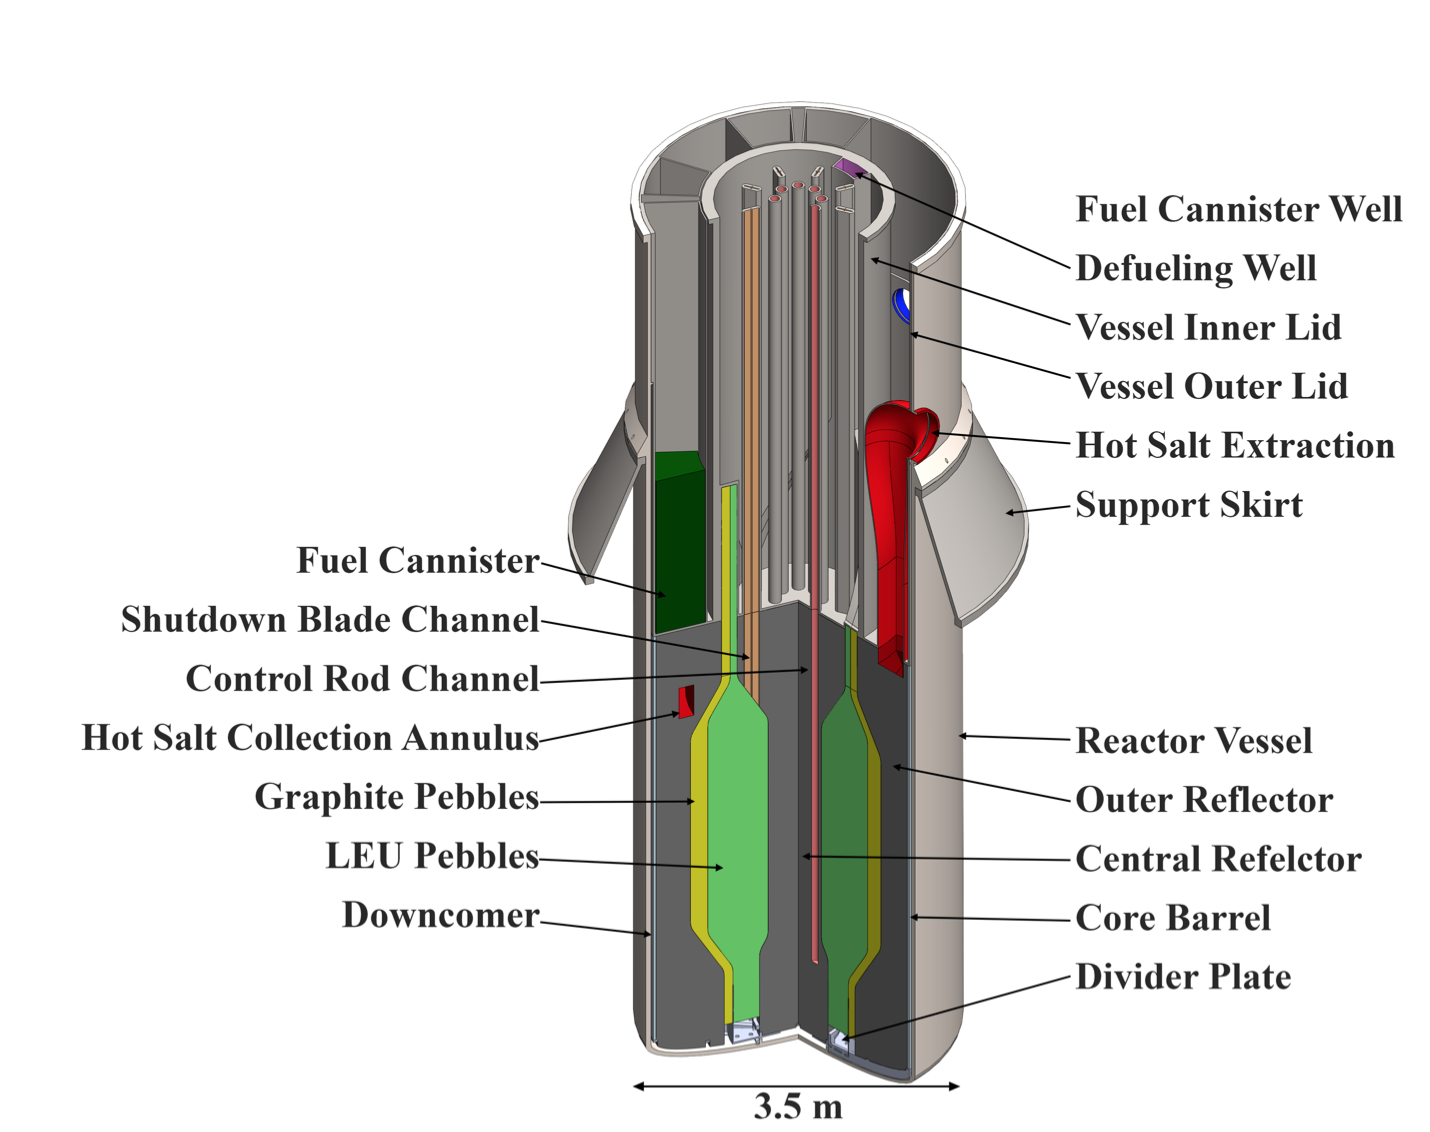
\includegraphics[width=\textwidth]{./images/design/Mk1_core_design.png}
  \caption{Schematic of Mk1 core geometry}
  \label{fig:Mk1_geom}
\end{figure}

\begin{table}
  \centering
  \begin{tabular}{lc}
    Parameter&Value\\
    \hline
    Thermal power, MW & 236\\
    Packing fraction for TRISO particles (\%)& 40\\
    Packing fraction for pebbles (\%)& 60\\
    Fuel enrichment (\%U-235)&19.9\\
    Flibe enrichment (\%Li-7)&99.999\\
    Number of fuel pebbles&470000\\
    Number of graphite pebbles&218000\\
    Number of TRISO particles per pebble & 4730\\
    Coolant inlet temperature, \degc & 600\\
    Coolant bulk-average outlet temperature, \degc & 700 \\
    Coolant flow, kg/s & 976\\
    Estimated coolant bypass, \% & 5\\
    Inner reflector radius, cm &35\\
    Average power density, $MW/m^3$ & 23 \\
    Volume of active fuel region, $m^3$ & 10.4 \\
    \hline 
  \end{tabular}
  \caption{Mk1 PB-FHR core design parameters}
  \label{tab:core_param}
\end{table}



As shown in figure \ref{fig:Mk1_geom}, a Mk1 core has an annular pebble bed region, consisting of fuel pebbles and graphite blanket pebbles, surrounded by center and outer graphite reflectors. 
A Mk1 core contains over 470000 three centimeter diameter fuel pebbles, smaller than the six centimeter ones used in helium cooled pebble-bed reactors and TMSRs. 
An illustration of the Mk1 fuel pebble and TRISO particle design can be found in figure \ref{fig:pb_triso_Mk1}. And the detailed geometry dimensions for Mk1 fuel elements can be found in table \ref{tab:Mk1_triso} and \ref{tab:Mk1_pb}.
Another difference from the TMSR SF-1 fuel is that the fuel pebbles in Mk1 are composed of three layers (instead of two): a low-density graphite core, a fuel layer and an outer graphite shell. The additional center graphite kernel in the Mk1 fuel pebbles provides neutron moderation and adjusts the overall pebble density so that they are slightly buoyant in the flibe salt. The pebble shell is made of dense graphite to protect the fuel by enhancing the structural strength of the pebble. In the annular fuel layer of each fuel pebble, thousands of TRISO particles are uniformly dispersed in a graphite matrix, each containing a fuel kernel, a porous buffer layer, an inner pyrocarbon layer, a silicon carbide layer and an outer pyrocarbon layer. The dimensions of these layers can be found in table \ref{tab:Mk1_triso}.
The smaller diameter and the annular design of the fuel pebbles doubles the heat transfer surface area per unit volume and shortens the thermal diffusion length to a half, enabling a higher power density while maintaining low peak fuel temperature, minimizing over-heating risk in postulated Anticipated Transient Without Scram (ATWS) accidents.

\begin{table}[h]
    \centering
    \begin{tabular}{lc}
        Layer & Dimension\\
        \hline\\
        Fuel kernel diameter & 400 $\mu m$ \\
        Buffer layer thickness & 100 $\mu m$\\
        PyC inner layer thickness &35 $\mu m$\\
        SiC layer thickness & 35 $\mu m$\\
        PyC outer layer thickness & 35 $\mu m$\\
        \hline\\
    \end{tabular}
    \caption{TRISO particle geometry in Mk1 PB-FHR \cite{Andreades2016}}
    \label{tab:Mk1_triso}
\end{table}

\begin{table}[h]
    \centering
    \begin{tabular}{lc}
        Layer & Dimension\\
        \hline
        Graphite core diameter& 25 mm \\
        Fuel thickness & 1.5 mm\\
        Shell thickness & 1 mm\\
        \hline\\
    \end{tabular}
    \caption{Fuel pebble geometry in Mk1 PB-FHR \cite{Andreades2016}}
    \label{tab:Mk1_pb}
\end{table}


The fuel pebbles are loaded from the bottom of the core and circulate in a slow upward motion across the core. In the time scale of the ATWS transients we simulate, ranging from several seconds to a few minutes, we can assume that the pebbles are fixed in space. After every pass, they are examined and reintroduced into the core until they reach the burnup limit. Meanwhile, newer pebbles are introduced in the core to compensate the deficiency in reactivity due to burnup. Online refueling allows the core to operate with limited excess reactivity and thus better safety prevision for control rod removal transients. Pebbles at different burnup level have different thermal and neutronic properties that need to be taken into account in the numerical models.



\begin{figure}
  \centering
  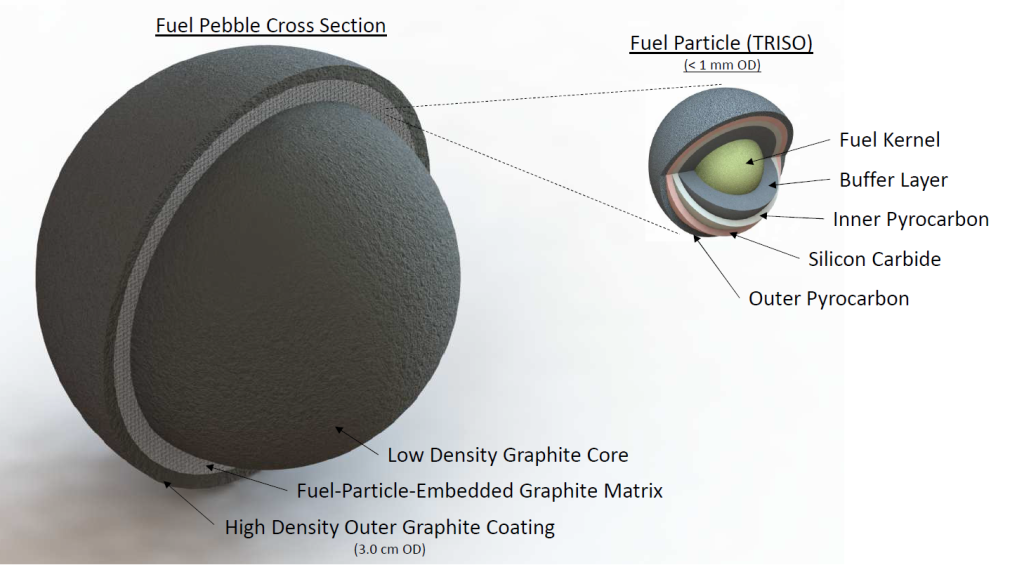
\includegraphics[width=0.85\textwidth]{./images/design/Mk1_fuel.png}
  \caption{Schematic of fuel pebbles and TRISO particles that are used in Mk1 PB-FHR}
  \label{fig:pb_triso_Mk1}
\end{figure}


Because of the large heat capacity of flibe salt, it is possible to have a low coolant flow rate in the core.
In the Mk1 core, about 30\% of the coolant flow enters from the downcomer at the bottom of the core while the rest is injected radially from the center reflector channels. The cross flow design reduces the pressure drop across the core and therefore reduces the total salt inventory and the flow resistance under natural-circulation for decay heat removal. 
Due to $^6Li$'s large absorption cross-section, the flibe salt needs to be enriched in $^7Li$ in order to achieve negative temperature reactivity feedback from the coolant. 
99.999\% is used as nominal flibe enrichment in this work.

% \begin{figure}
%     \centering
%     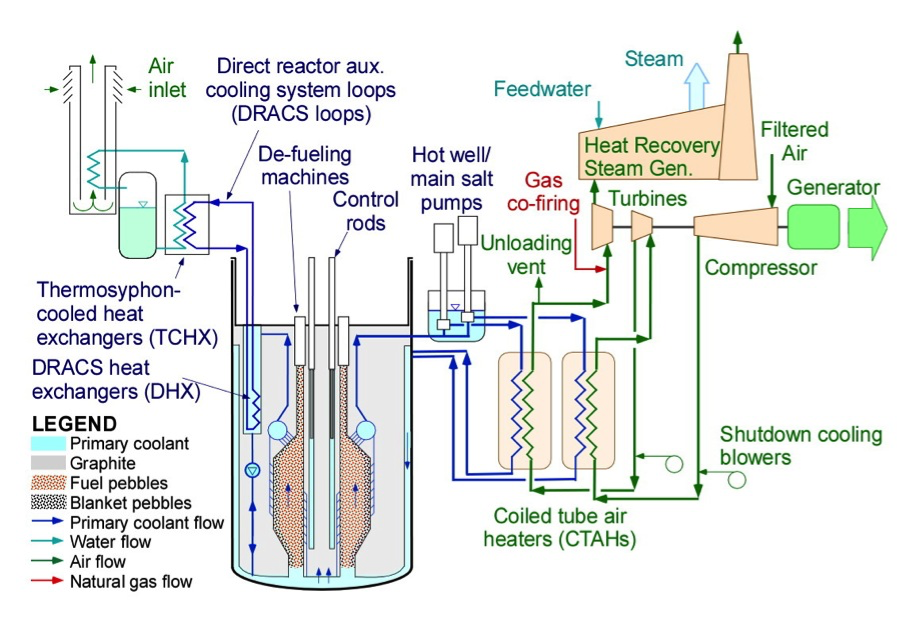
\includegraphics{design/Mk1_flow_overall.png}
%     \caption{Mk1 primary coolant flow paths}
%     \label{fig:mk1_flow}
% \end{figure}


%As shown in figure \ref{fig:Mk1_geom}, the Mk1 core is composed mainly by fuel and blanket pebbles, reflectors, and reactivity control elements.
% The design parameters are in table \ref{tab:core_param}.

In addition to the graphite material inside the fuel elements, a Mk1 core contains multiple graphite components, including an outer reflector and a center reflector that surround the core, providing neutron moderation and reflection. 
% Coolant channels are embedded in the graphite blocks to carry the heat deposited in reflectors through gamma, neutron and thermal radiation.
And between the fuel pebbles and the outer reflector is a 20 cm thick ring of graphite pebbles, serving as a dynamic reflector. The graphite pebbles can be unloaded through the defueling chute at the top and loaded from the bottom. It can also be replaced by thorium-loaded pebbles in a breeder reactor design, a concept not investigated in this thesis. 
Studies on granular dynamics \cite{Laufer2013} have shown that the pebbles move upward in the core with limited radial motion. Therefore, the fuel region and the blanket regions remain separated as the pebbles circulate and is modeled as separate regions in this work.

In addition to the online refueling regime for long term reactivity compensation, Mk1 uses eight Boron Carbide control rods for operating reactivity control and eight emergency blades for reserve shut-down. The control rod channels are located in the center reflector, where neutron flux is the highest, for an efficient reactivity control via neutron absorption. 
The control rods are inserted from the top of the core and thus can remain effective in case of earthquake when the fuel pebbles are densified toward the top of the core.


%\begin{figure}[ht]
% \centering
% 
\includegraphics[width=0.5\textwidth]{./images/design/CR_illustration.png}   
% \caption{Illustration of control rod cross-section in a Mk1 center reflector, shown in yellow}
% \label{fig:cr}
%\end{figure}






\section{Monte Carlo modeling for Mk1}
\label{sec:Mk1_serp}

\begin{table}
 \centering
 \begin{tabular}{lcccc}
    \multicolumn{2}{c}{Component} & Density & Material & Temperature\\
    &  [g/$cm^3$] & & [K]\\
    \hline\\
    \multirow{2}{*}{Fuel} & Shell & 2 & graphite & 900\\
                          & Kernel & 2 & graphite & 1000\\
                          & Coolant & 1.95 & flibe (0.99999) & 1000\\
                          \hline\\
    \multirow{5}{*}{Triso} & Matrix & 2 & graphite & 1000\\
                           & Kernel & 10.5 & UC0.5O1.5 & 1000\\
                           & Buffer & & graphite & 1000\\
                           & iPyC & & graphite & 1000\\
                           & SiC & & SiC & 1000\\
                           & oPyC & & graphite & 1000\\
                           \hline\\
    \multirow{2}{*}{Blanket} & pebbles & & graphite & 900\\
                             & coolant &  1.97 & flibe (0.99999) & 900\\
                             \hline\\
    \multicolumn{2}{c}{Center Reflector} & 1.74 & graphite & 900\\
    \multicolumn{2}{c}{Control rods}& 2.4 & Natural B4C & 900\\
    \multicolumn{2}{c}{Control rods coolant}& 1.97 & flibe (0.99999) & 900\\
    \hline\\
    \multicolumn{2}{c}{Outer Reflector} & 1.74 & graphite with boron & 900\\
    \multicolumn{2}{c}{Coolant channel outer reflector}& & graphite and flibe & 900\\
    \hline\\
     \multicolumn{2}{c}{Core Barrel} & 8 & SS316 & 900\\
     \multicolumn{2}{c}{Reactor Vessel}& 8  & SS316 & 900\\
 \end{tabular}
 \caption{Material and temperature for each core component in the reference Mk1 Serpent model. The isotope composition of the stainless steel in core barrel and vessel is given in table \ref{tab:ss316}\cite{ESPI}.}
 \label{tab:matT}
\end{table}




\begin{table}
  \centering
  \begin{tabular}{cccccccccc}
    Isotope&C&Fe&Ni&Cr&Mo&Si&Mn&S&P\\
    \hline\\
    Fraction(\%wt)&0.080&65.345&12.000&17.000&2.500&1.000&2.000&0.030&0.045
  \end{tabular}
  \caption{Nominal composition of stainless steel 316, density 8.03$g/cm^3$}
  \label{tab:ss316}
\end{table}

\begin{figure}
  \centering
    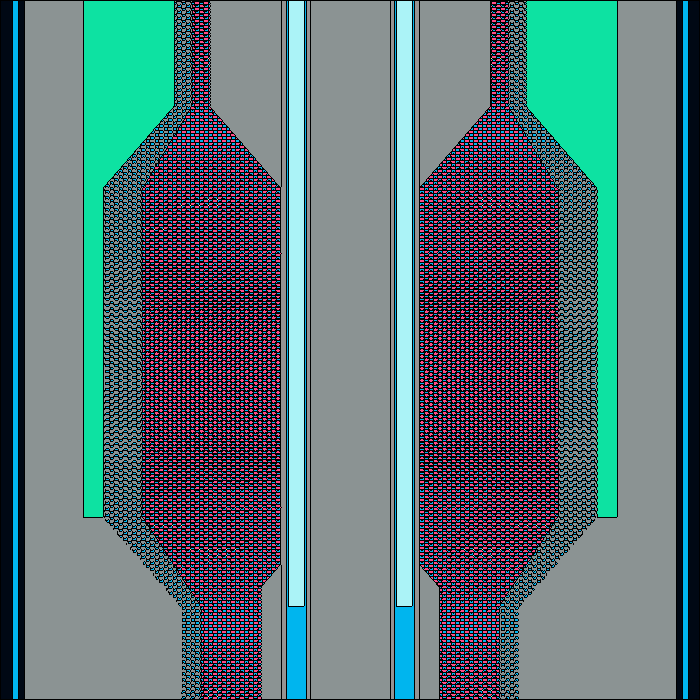
\includegraphics[width=0.49\textwidth]{design/serp_full_core_geom2.png}
    ~
    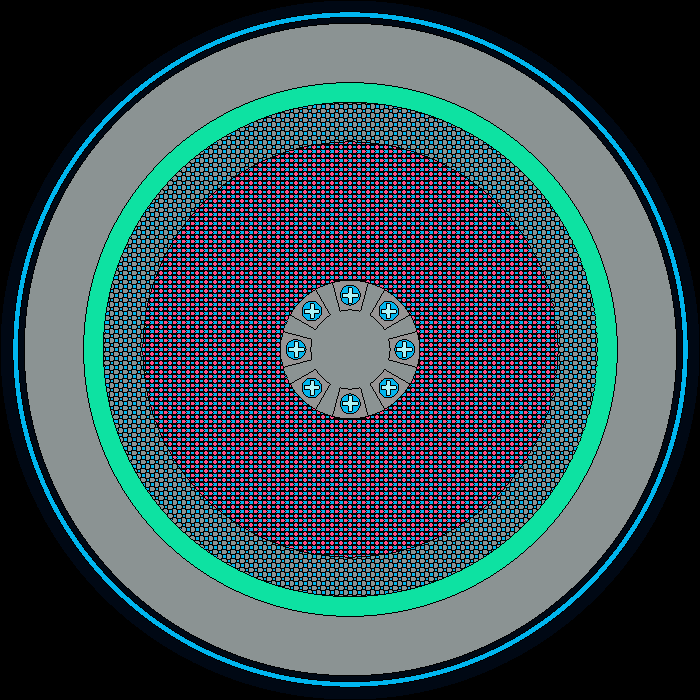
\includegraphics[width=0.49\textwidth]{design/serp_full_core_geom3.png}
    ~
    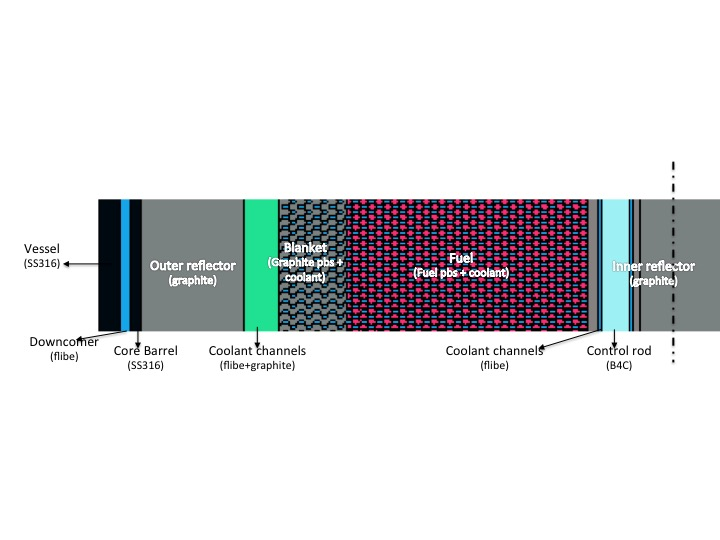
\includegraphics[trim={0, 6cm, 0, 6cm}, clip, width=0.8\textwidth]{design/Mk1_serp_color_legend.jpg}
  \caption{Geometry of the Monte Carlo model for Mk1 in Serpent (View from the front, the top, and color legend), with all control rods fully inserted}
  \label{fig:serp_Mk1}
\end{figure}

A Monte Carlo model is made for Mk1 PB-FHR in Serpent \cite{Serpent2015} to study detailed neutronics properties in the core and to generate parameters used by deterministic codes. Cross-section data from the ENDF/B-VII.0 nuclear data library is used for this model. The full core model is run with 10000 particles per cycle for 10000 cycles where the first 500 are skipped when computing result statistics. Because of the high fidelity of Monte Carlo based code, these models are also used to generate reference results to benchmark other models. 

As shown in figure \ref{fig:serp_Mk1}, the model is composed of center reflector, fuel pebble region, blanket pebble region, outer reflector, vessel, downcomer and core barrel, with uniform nominal material compositions and temperatures in table \ref{tab:matT}.
The model geometry is based on the design report \cite{Andreades2016} with some simplifications in view of computation cost. 
The next sections describes how each components are modeled, including the assumptions and simplifications with justifications.





\subsection{Center reflector}

Figure \ref{fig:Mk1_cr} shows the design of the center reflector. It is composed by a number of graphite blocks, with small gaps between each other to allow for thermal expansion and radiation induced swelling of the graphite material. It is modeled as a single piece because the gaps are negligible comparing to the neutron mean free path in graphite. The center reflector has coolant injection channels that deliver coolant to the fuel region through the injection holes and slot, which are not modeled in this neutronic model because the small amount of flibe in the channels has negligible effects on the core neutronic behaviour.

\begin{figure}
    \centering
    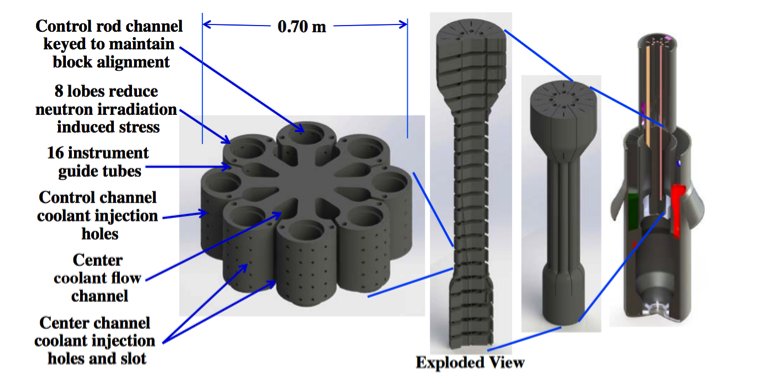
\includegraphics[width = \textwidth]{images/design/Mk1_cr_design.png}
    \caption{Center reflector design}
    \label{fig:Mk1_cr}
\end{figure}



\begin{table}[h]
\centering
  \begin{tabular}{lc}
  \hline
     Parameter  & Value  \\
     \hline
       Number of control rods & 8\\
       Diameter of control rods channels, cm & 10\\
       Width of control rods, cm & 8\\
       Thickness of control rods, cm & 2\\
       Bottom height (fully inserted), cm & 112.5 \\
       Bottom height (fully retracted), cm & 492.85\\
       Density, kg/m3 & 2400\\
       Material & Boron Carbide\\
       \hline
  \end{tabular}
  \caption{Design specification for control rods in Mk1}
  \label{tab:cr_dim_Mk1}
\end{table}

In a Mk1 core, the thermal neutron flux peaks in the center reflector, which makes it the best location for control rod channels. In fact, the center reflector houses eight control rod channels (design details in table \ref{tab:cr_dim_Mk1}). In each channel, a cross shaped control rod can be inserted to maintain criticality under normal operation conditions or to aid shutdown blades to shutdown the reactor under accident conditions. The design of the channels and the material used in the channels need to be evaluated carefully because of the high impact on neutronics. 
In order to study the feasibility of adding metallic (stainless steel) or ceramic (silicon carbide) liners to the channels to provide structural reinforcement, a Monte Carlo model with equilibrium fuel composition is used to compute $\Delta \keff$, the decrease in the multiplication factor, due to the presence of the liners. 
To estimate the maximum absorption effect of the liners on neutron flux, the control rods are not inserted in the model, i.e. the channels are filled with flibe coolant.

\begin{table}
  \centering
  \begin{tabular}[h]{cccc}
    Material&Thickness [mm]& $\Delta$ \keff \\
    \hline\\
    %Non & 0.967163 & 0.00018\\
    SS316 & 5 & 0.08139\\
    SS316 & 3 & 0.06798\\
    SS316 & 10 & 0.09639\\
    %Graphite & 5 & 0.00412\\
    Zr & 5 & 0.01196\\
    SS316 without Ni & 5 & 0.08033 \\
    SiC & 5 & 0.01070
  \end{tabular}
  \caption{Drop in \keff due to different control rod liner materials and configurations}
  \label{tab:ssliner}
\end{table}

Table \ref{tab:ssliner} lists the drop in \keff with different liner materials and thicknesses. Stainless steel reduces the \keff considerably, over 6000~pcm for 3~mm and almost 10000~pcm for 10~mm due to its high capture cross-sections and the central location of the channels. The effect remains consistent when the thickness is between 1~mm and 3~mm, the reduction in \keff are within statistical error.
Zirconium, on the other hand, is more transparent to neutrons, but is also easily corroded by the coolant salt. Adding three millimeters of zirconium liners results in smaller reduction in \keff. The SiC liner has also smaller effect on \keff comparing to stainless steel and can potentially be a candidate material for the liner, given its neutronic performance as well as high temperature resistance. Carbon fiber reinforced composites (CFRCs) are also candidates, since they will have the same neutronics effects as graphite





\subsection{Fuel region}

\begin{figure}[h]
  \centering
  %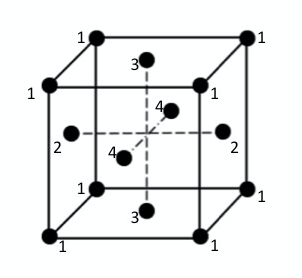
\includegraphics[width=0.45\textwidth]{./images/design/fuel_loading_active.png}
  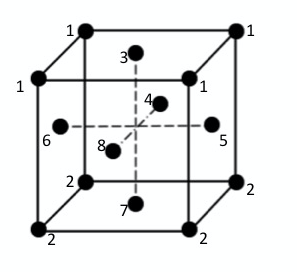
\includegraphics[width=0.5\textwidth]{./images/design/fuel_loading_wall.png}
  \caption{Schematic of equilibrium fuel loading in a representative unit cell, numbers denote burnup levels}
  \label{fig:burnups}
\end{figure}


We model the pebble packing as a Face-Centered Cubic(FCC) lattice with a packing fraction of 60\%. The flibe salt fills the space between fuel pebbles. The optimal coolant enrichment is determined in view of safety criteria and economics viability. 0.9999 enriched flibe is used in the current model to ensure negative coolant reactivity feedback. 

Either the fresh or the equilibrium fuel composition can be used in the model. Mk1 adopts an online refueling regime. Starting from fresh fuel, the pebbles circulates in the core for, on average, eight times. During the online refueling cycle, the fuel pebbles gradually reaches asymptotic packing and burnup distribution. An equilibrium unit cell containing equal volume of pebbles at eight different burnup levels, illustrated in figure \ref{fig:burnups}, was computed with a depletion model\cite{Cisneros2013} under an online refueling scheme. 




\subsection{Blanket pebble region}
Graphite blanket pebbles are also modeled in a FCC lattice with the same packing fraction and pebble dimension as the fuel pebble region. The coolant material in this region also has the same composition and temperature as that in the fuel region. A clear cut is made between the blanket and the fuel region in the model, while in reality a small number of pebbles might migrate into each other zones in the vicinity of the interface. 


\subsection{Outer reflector}
The outer reflector is made of graphite with boron. 
Coolant channels in the outer reflector are modeled as a fictitious material with 60\% (volumetric) graphite and 40\% (volumetric) flibe in a 10 cm annular band in the active regions and extends up to the top of the core, as shown in green in figure \ref{fig:serp_Mk1}.



\subsection{Outer layers}
Outside of the graphite reflector lies the layers for structural integrity, namely the core barrel and the vessel.
The cavity between core barrel and the vessel is filled with flibe salt. 
A shield can be added between the outer reflector and core barrel to protect the metallic material. 
The dimension of the outer layers with or without the shield is shown respectively in table \ref{tab:ol_shield} and table \ref{tab:ol_no_shield}. 

\begin{table}
  \centering
  \begin{tabular}{llll}
    Component & Outer Radius(cm) & Material\\
    Shield & 164.7 & Boron Carbide\\
    Core Barrel & 168 & SS316\\
    Downcomer & 170 & Flibe\\
    Vessel & 175 & SS316
  \end{tabular}
  \caption{Dimension and material of Mark I core outer annular layers with shield\cite{Cisneros2013}}
  \label{tab:ol_shield}
\end{table}

\begin{table}
  \centering
  \begin{tabular}{llll}
    Component & Outer Radius(cm) & Material\\
    Core Barrel & 167.2 & SS316\\
    Downcomer & 170 & Flibe\\
    Vessel & 175 & SS316
  \end{tabular}
  \caption{Dimension and material of Mark I core outer annular layers without shield\cite{Andreades2016}}
  \label{tab:ol_no_shield}
\end{table}




%\begin{table}
%  \centering
%  \begin{tabular}{lccccc}
%    Code & Keff & Standard & Particles& Skipped & Total\\
%    & & deviation & per & cycles &cycles \\
%    & & [pcm] & cycle& & \\
%    \hline\\
%    MCNP & 0.94199 & 12 & 100000 & 200 & 500\\
%    Serpent & 0.94144 & 11 & 100000 & 200 & 500\\
%    \hline\\
%    $\Delta$ Keff[pcm] & 55 && & \\
%    \hline
%  \end{tabular}
%  \caption{Comparison of criticality calculation results between MCNP and Serpent for full core model}
%  \label{tab:full_core_res}
%\end{table}

% Comparison with Tommy's model: keff, temperature feedback, control rod worth

% The Los Alamos Natlional Laboratory's MCNP code is also widely used Monte Carlo code for nuclear reactor physics. It is used in this project to benchmark Serpent models.







\section{Multiphysics modeling for Mk1}
\label{sec:comsol_mk1}


A coupled thermal-hydraulics and neutronics model is implemented for Mk1 for transient analysis based on the methodology developed in section \ref{sec:comsol}. The model solves multi-group diffusion equations for neutronics, where the cross-sections are generated for each component using the Serpent model discussed in the previous section. 
The overall geometry (figure \ref{fig:Mk1_comsol_model}) is the same as the Monte Carlo model discussed in the previous section, except that the sharp corners in the geometry are rounded for a more realistic flow field.


\begin{figure}
    \centering
    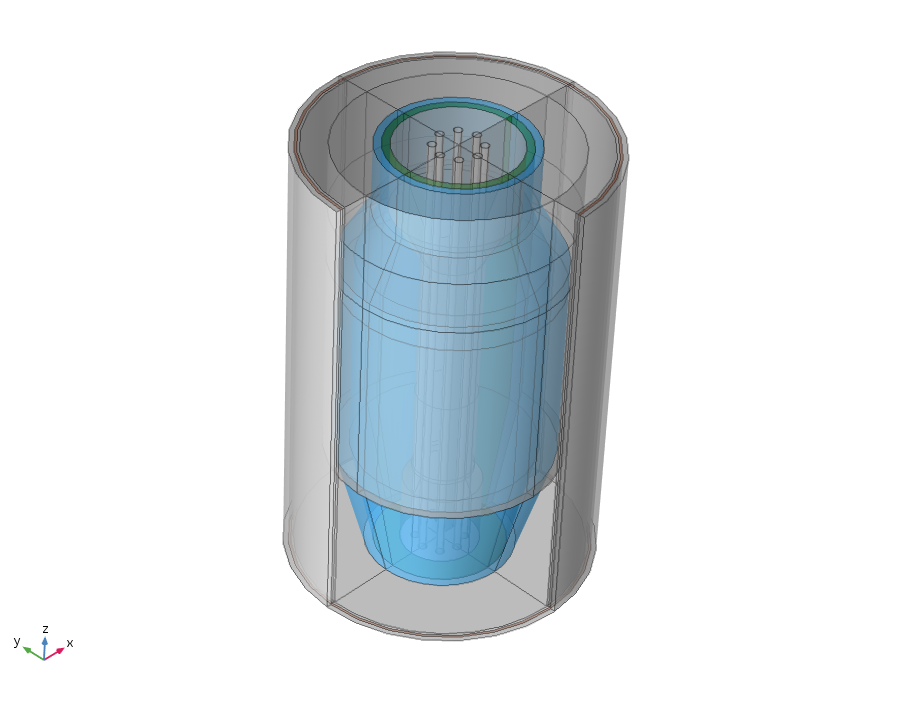
\includegraphics[width=0.8\textwidth]{images/diffusion/mk1/Mk1_comsol.png}
    \caption{Schematic of the Mk1 multiphysics model geometry. Green region is the fuel pebble region and blue region is the blanket pebble region.}
    \label{fig:Mk1_comsol_model}
\end{figure}



\subsection{Porous media model for coolant}



The porous media formulation (discussed in section \ref{sec:comsol}) is used to model the pebble-bed flow field and heat transfer in Mk1. The model uses salt thermal-physical properties in appendix \ref{chap:mat}. 

The convective heat transfer between the fuel surface and the coolant is modeled using the Wakao correlation \cite{Wakao1979}, and the Ergun correlation \cite{Ergun1949} is used for pressure loss computation.
The Ergun constants, $E_1$ and $E_2$, depend on conditions like flow regime (e.g. Reynolds number), surface texture (e.g. roughness), pebble packing (e.g. porosity) and container shape (e.g. bed-pebble diameter ratio), and  should ideally be measured for each pebble bed. However, without the measurements for Mk1 pebble bed, the values in the original Ergun correlation are used in this work. Table \ref{tab:ergun_coef} shows the Ergun coefficients and the constant used in COMSOL for defining Ergun correlation in the momentum equation. The effect of the uncertainty on the results of the coupled models should be studied to decide if dedicated measurements are necessary.

\begin{table}
\centering
  \begin{tabular}{lc}
    Parameter & Value\\
    $E_1$ &150 \\
    $E_2$ &1.75\\
     $C_F$ & 0.52 \\
  \end{tabular}
  \caption{Pressure drop correlation parameters used in the porous media model}
  \label{tab:ergun_coef}
\end{table}



Pressure boundary conditions are imposed on outlet surfaces. A velocity profile or an overall flow rate is specified for inlet surfaces. The boundary conditions are optimized in section \ref{sec:pressure} to achieve efficient cooling and limited pressure drop.
    

As shown in figure \ref{fig:mk1_flow}, the coolant flows through the Coiled Tube Air Heaters(CTAHs) after exiting the core and deposits heat to the power conversion system before coming back to the core. Thus during long transients that last more than the coolant circulation time, the coolant inlet temperature will be affected by the coolant coming back with a different temperature. To represent the primary loop, during longer transient scenarios, a simplified heat exchanger model is added to the core. In the future, coupling between the core model and system model would give a more realistic representation of transients that affects components outside of the core.
The heat transfer rate in CTAHs is computed using the following equations. The heat exchanger efficiency and parameters about the air flow are assumed to remain constant during the simulated transients because the power conversion system is not affected.

\begin{align}
    Q_{real} = Q_{max} * \eta\\
    Q_{max} = C_{min}(T_{salt,in} - T_{air, in})
\end{align}

where:\\
$Q_{real}$ = real thermal power, W\\
$Q_{max}$ = maximum attainable thermal power in counter-flow heat exchanger, W\\
$\eta$ = heat exchanger efficiency = 0.9\\
$T_{air, in}$ = cold air inlet temperature = 418.6[\degc] \\
$T_{salt, in}$ = hot salt inlet temperature\\
$C_{min} = min((\dot{m}C_p)_{air}, (\dot{m}C_p)_{salt})$ = 461540[J/K]\\
$c_p$ = specific heat\\
$\dot{m}$ = mass flow rate\\

 

\subsection{Multi-scale model for the fuel region}

The fuel region is divided radially and axially into 6 zones, based on the different neutron spectrum characteristics \cite{Cisneros2013}, and in each zone a different set of cross-sections is generated as a multi-variable linear function of the flibe density and logarithm of fuel temperatures. 
The benefit of computing the temperature profile inside the fuel elements is demonstrated in section \ref{sec:TMSR_transients} and thus is also used for Mk1 models.
The fuel kernel in each TRISO particle is divided into three layers with equal volume, i.e. same amount of fuel, and the temperature in each layer is computed at each time step using the multi-scale heat transfer model developed in section \ref{sec:comsol}.

\begin{figure}
     \centering
     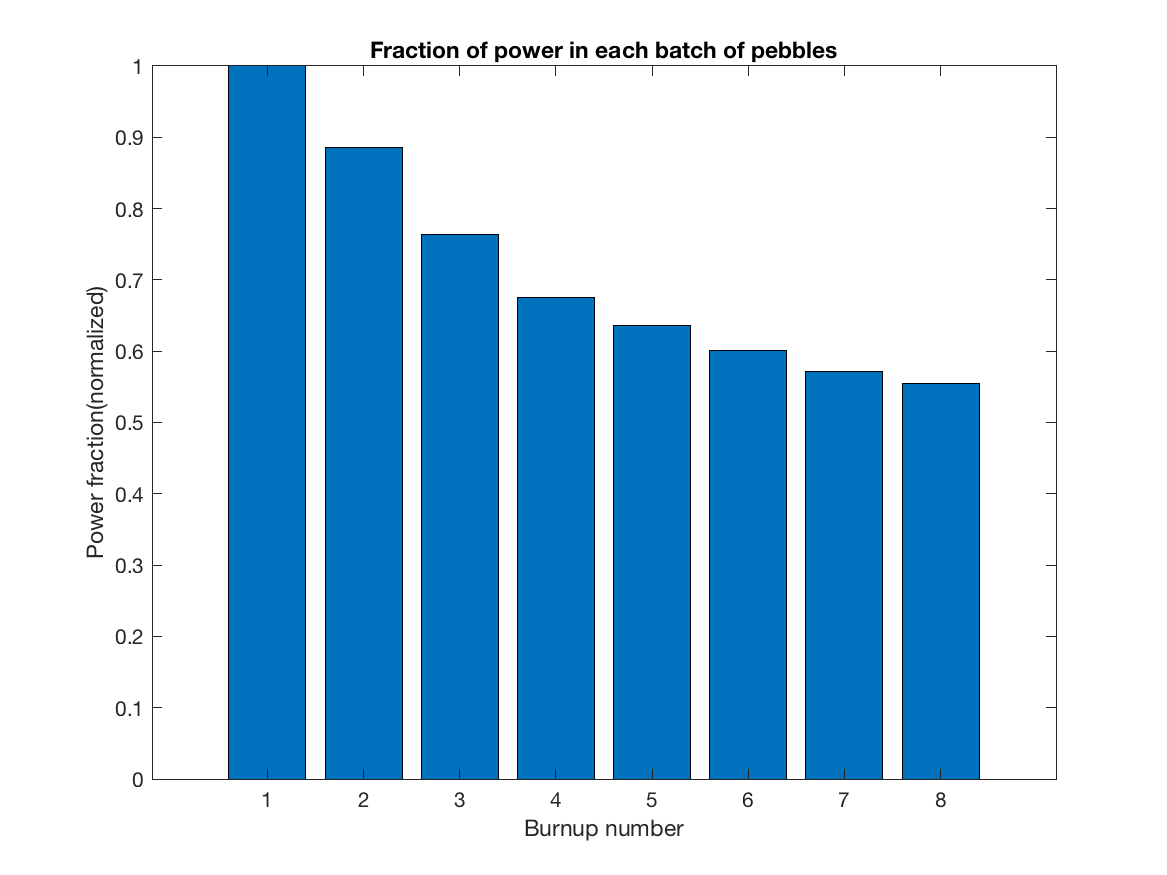
\includegraphics[width=0.8\textwidth]{images/diffusion/mk1/power_barchart.png}
     \caption{Fraction of power generated in pebbles of each burnup level}
     \label{fig:power_fraction}
\end{figure}

 \begin{figure}[h]
  \centering
  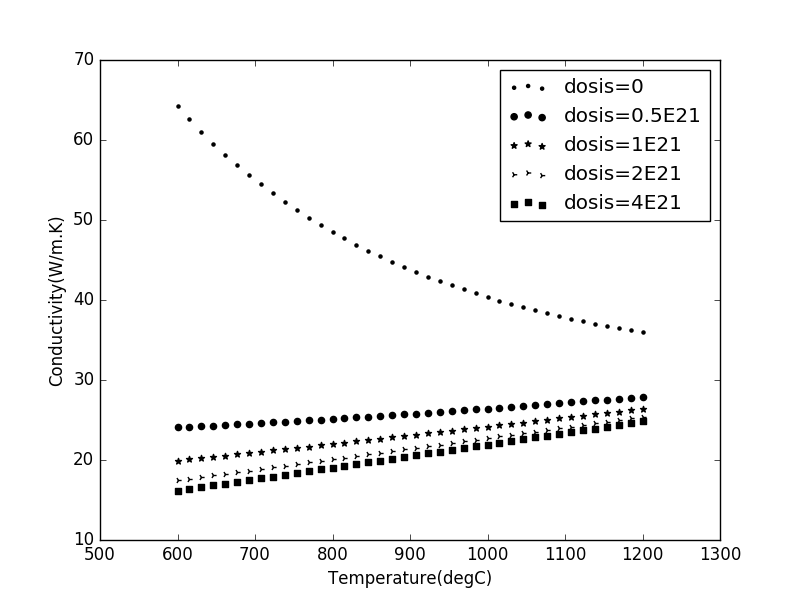
\includegraphics[width=0.7\textwidth]{./images/design/fuel_conductivity.png}
  \caption{Fuel pebble conductivity as a function of temperature and irradiation dose(data from \cite{IAEA2000})}
  \label{fig:fuel_conductivity_mk1}
\end{figure}

A Mk1 core contains fuel pebbles with various levels of burnup and approaches the asymptotic packing and burnup distribution as the pebbles flow slowly across the core during an online refueling campaign. To model a core with equilibrium fuel in the multiphysics model, the temperatures in pebbles at each burnup level are computed. As the fuel elements undergo irradiation, its ability in generating power degrades due to the change in fuel composition. 
A fresh pebble would produce almost twice of power than a pebble that is at its last pass before reaching the burnup limit, as shown in figure \ref{fig:power_fraction}. The fraction of power that is generated in pebbles of each pass is tallied using the Monte Carlo model and is used as input for the multiphysics model with equilibrium fuel. 

Figure \ref{fig:fuel_conductivity_mk1} shows the fuel pebble equivalent thermal conductivity based on fast neutron dose and the temperature at which the pebble is irradiated, computed based on the empirical formula in equation \ref{eq:k_pb_mk1}.
The conductivity varies between about 15 W/m.K to more than 60 W/m.K depend on the irradiation damage and temperature. Most of the degradation occurs during the first pass of the pebbles in the core. To simplify the model, a constant thermal conductivity is used for pebbles of each pass, as shown in table \ref{tab:k_bu}.


 


\begin{equation}
  \lambda = 1.2768*(\frac{0.6829-0.3906*10^{-4}T}{dosis+1.931*10^{-4}T}+1.228*10^{-4}T + 0.042)
  \label{eq:k_pb_mk1}
\end{equation}

where $\lambda$ is in the unit of W/cm.K, T is the temperature in degree Celsius (T<1200$^{\circ}C$), and dosis is the fast neutron irradiation dose in $10^{21}$.



\begin{table}[h]
    \centering
    \begin{tabular}{lcccccccc}
         Pass No. & 1 & 2 & 3 & 4 & 5 & 6 & 7 & 8  \\
         k[W/K.m] & 40 & 17 & 17 & 17 & 17 & 17 & 17 & 17 \\ 
    \end{tabular}
    \caption{Thermal conductivity of fuel pebbles at different burnup levels}
    \label{tab:k_bu}
\end{table}





 For a core with only fresh fuel pebbles, pebble wise equivalent properties are used for general modeling and more specific layer-wise properties are used in case of multiscale mode where each layer is modeled and their temperature is computed at each time step. The thermal-physical properties of the fuel elements are listed in table \ref{tab:triso_prop_mk1} and \ref{tab:pb_prop_mk1}.


\begin{table}[h]
  \centering
  \begin{tabular}{cccc}
    Region&Density&Conductivity&Specific heat\\
    &[g/cc]&[W/m.K]&[J/kg/K]\\
    \hline\\
    Kernel & 10.5 & 3.5 & 400\\
    Buffer & 1.0 & 0.5 & 2000\\
    IPyC & 1.9 & 4.0 & 2000\\
    SiC & 3.2 & 30 & 1300\\
    OPyC & 1.9 & 4.0 & 2000\\
    Coating* & 1.89 & 0.76 & 1736\\
  \end{tabular}
  \caption{Nominal material properties of Mk1 fuel element used in the models \cite{Hu2010}\cite{FHR2013}. *Coating combines all the non-power-generating layers in a TRISO particle.}
  \label{tab:triso_prop_mk1}
\end{table}


\begin{table}
  \centering
  \begin{tabular}{cccc}
    Region&Density&Conductivity&Specific heat\\
    &[g/cc]&[W/m.K]&[J/kg/K]\\
    \hline\\
    Kernel & 1.74  & 193 & 684\\ %density from design report, nominal density for graphite
    Fuel & 1.81 & 15 & 1744\\
    Shell & 1.96 & 193 & 684\\
    Pebble* & 1.85 & 17 & 1700 \\
  \end{tabular}
  \caption{Nominal material properties of Mk1 fuel pebble used in the models \cite{Hu2010}\cite{FHR2013}. *Pebble: pebble-wise material properties}
  \label{tab:pb_prop_mk1}
\end{table}

 
 



 


\newpage 
\subsection{Control rod modeling and verification}
The control rods are super-homogenized radially with a portion of surrounding graphite to make the diffusion model more adequate to be used in this area. Also, the channels are discretized axially into multiple segments and two sets of cross sections are generated for each of the segments with or without control rod. This process generates a step function of cross-section as a function of height. 

\begin{equation}
    \Sigma(z) = \sum_{seg = i}^{N} \Sigma_{seg, flibe}*(z<z_{rod}) + \Sigma_{seg, rod}*(z>=z_{rod})
\end{equation}

where $\Sigma$ is a cross-section as a function of the height, $z_{rod}$ is the control rod position, $\Sigma_{seg, flibe}$ is the cross-section value when the channel segment is filled with flibe, and $\Sigma_{seg, rod}$ is the cross-section value when the channel segment is inserted with control rod. 

To verify the capability of the COMSOL model in modeling the control rod effect on power distribution, power profiles with different control rod configurations are computed and compared to the results from a Monte Carlo reference model. 
For the comparison, both models use uniform nominal material temperatures and equilibrium fuel composition.

Figure \ref{fig:mk1_no_power} and \ref{fig:mk1_no_rods_power} shows the power distribution in the core when no rods are inserted. Figure \ref{fig:mk1_full_power} and \ref{fig:mk1_full_rods_power} shows the power distribution in the core when all the rods are fully inserted.
Also, for a more quantitative comparison, all the control rods are moved together to different heights and the change in the multiplication factor is compared between the COMSOL model and the Serpent model, as shown in figure \ref{fig:delta_keff_cr}. 



\begin{figure}
\centering 
  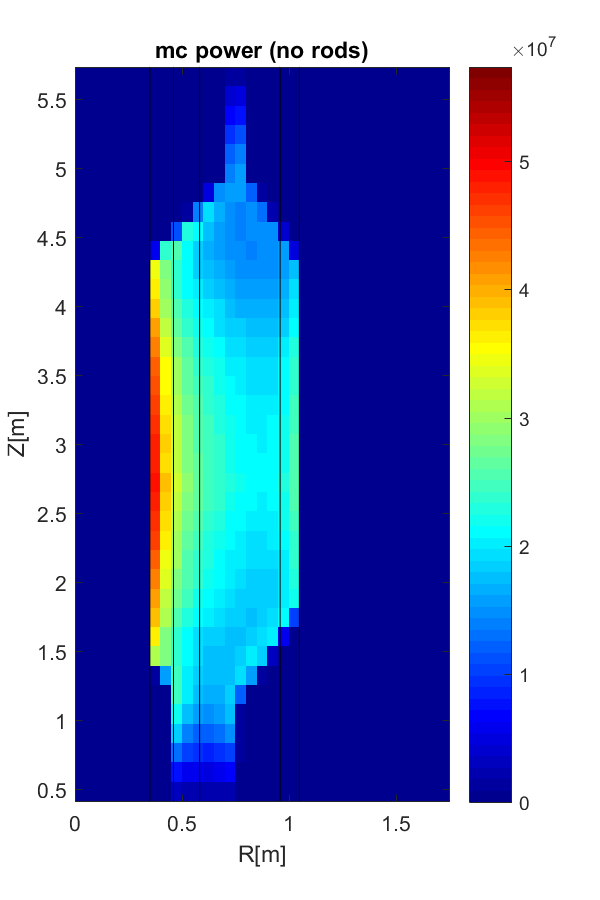
\includegraphics[width=0.4\textwidth]{benchmark_mk1/mc_no_rods.png}
  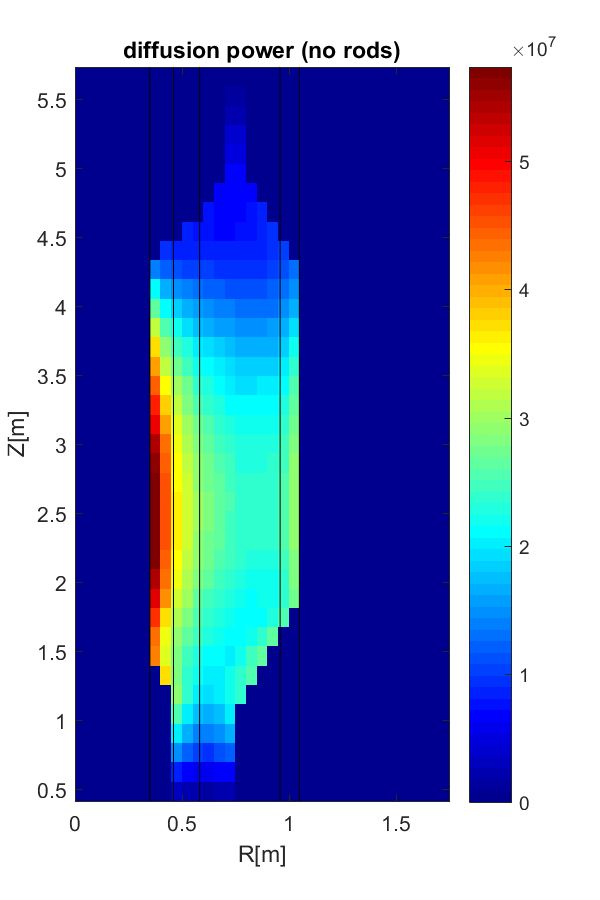
\includegraphics[width=0.4\textwidth]{benchmark_mk1/diffusion_no_rods.png}
  \caption{Steady state power distribution from the Monte Carlo reference model and from the COMSOL model (nominal conditions, no control rods inserted in the core)}
  \label{fig:mk1_no_power}
\end{figure}

\begin{figure}
\centering 
  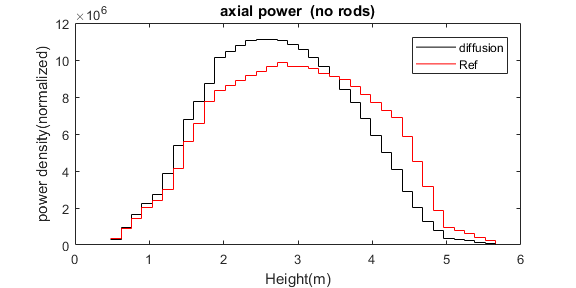
\includegraphics[width=0.49\textwidth]{benchmark_mk1/axial_no_rods.png}
  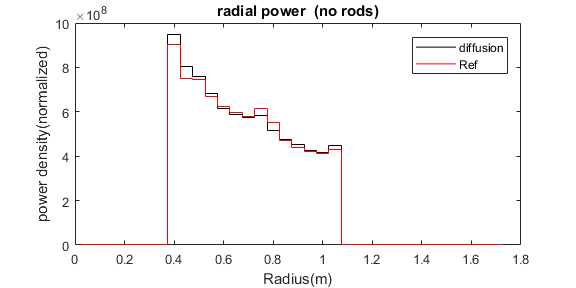
\includegraphics[width=0.49\textwidth]{benchmark_mk1/radial_no_rods.png}
  \caption{Steady state neutron flux distribution from the Monte Carlo reference model and from the COMSOL model (nominal conditions, no control rods in the core)}
  \label{fig:mk1_no_rods_power}
\end{figure}

\begin{figure}
\centering 
  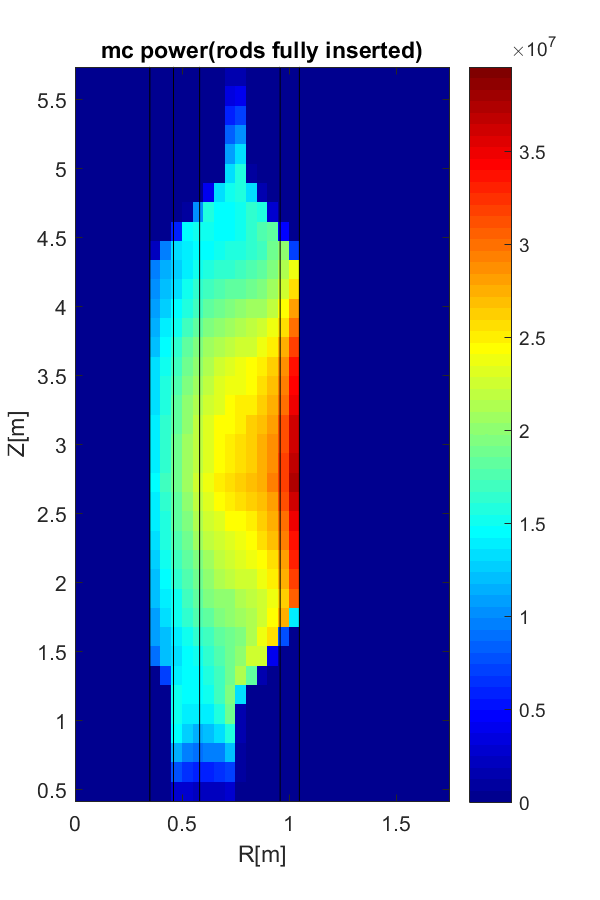
\includegraphics[width=0.4\textwidth]{benchmark_mk1/mc_rods_fully_inserted.png}
  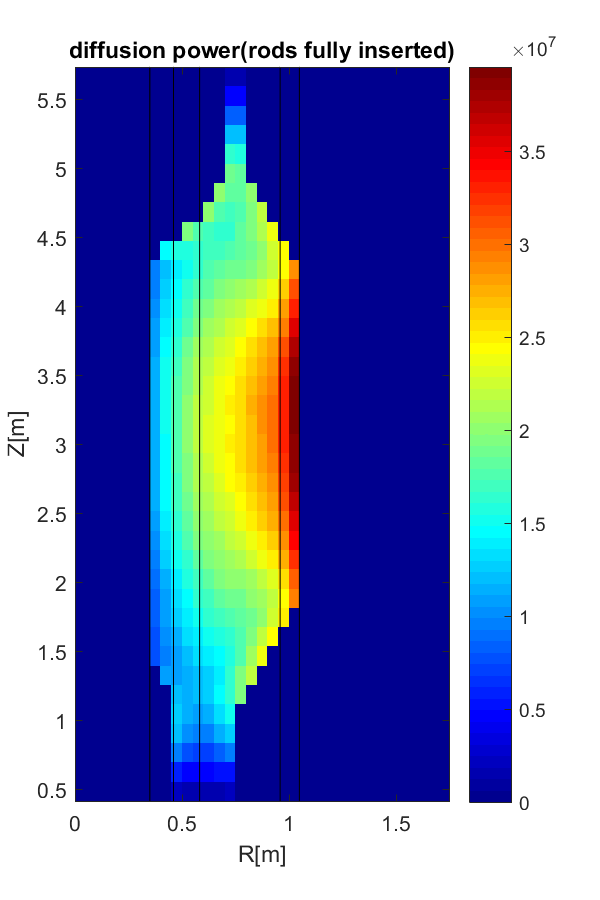
\includegraphics[width=0.4\textwidth]{benchmark_mk1/diffusion_rods_fully_inserted.png}
  \caption{Steady state power distribution from the Monte Carlo reference model and from the COMSOL model(nominal conditions, control rods fully inserted in the core)}
  \label{fig:mk1_full_power}
\end{figure}

\begin{figure}
\centering 
  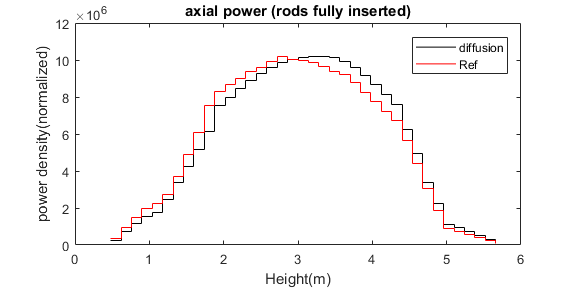
\includegraphics[width=0.49\textwidth]{benchmark_mk1/axial_rods_fully_inserted.png}
  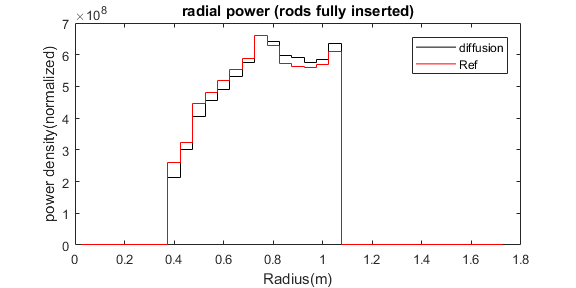
\includegraphics[width=0.49\textwidth]{benchmark_mk1/radial_rods_fully_inserted.png}
  \caption{Steady state neutron flux distribution from the Monte Carlo reference model and from the COMSOL model(nominal conditions, control rods fully inserted in the core)}
  \label{fig:mk1_full_rods_power}
\end{figure}



\begin{figure}
    \centering
    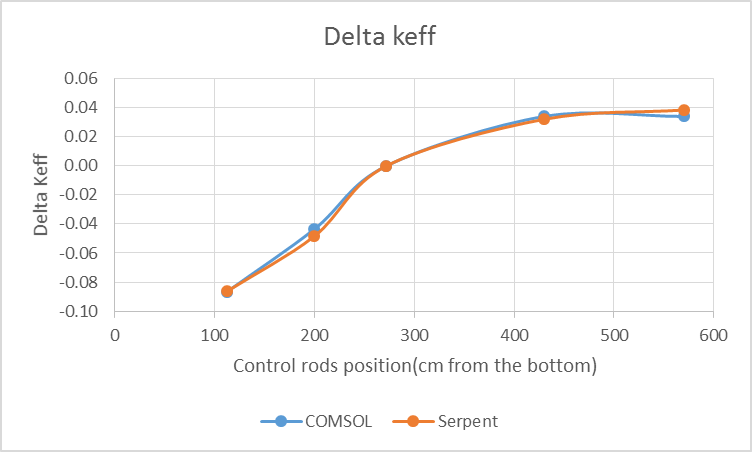
\includegraphics{benchmark_mk1/delta_keff_cr.png}
    \caption{Change in \keff with control rod positions}
    \label{fig:delta_keff_cr}
\end{figure}

\newpage
\section{Steady state Mk1 core analysis and design optimization}
\label{sec:mk1_ss}

The first part of the section discusses steady state characteristics for Mk1 core, assuming that the control rods are not inserted in the core and the core is loaded with fresh fuel. The effect of coolant inlet and outlet channels on the core behaviour is investigated in the second part of this section using coupled thermal-hydraulics and neutronics models. 




\subsection{Power and flux distribution}

Steady state power,thermal and fast neutron flux distribution are shown in figure \ref{fig:mk1_flux}. 
As shown in the figure, the thermal flux peaks in the center reflector, in the graphite blanket pebble area and the outer reflector. As a result, the power peaks in the vicinity of the reflectors when the thermal neutrons enters the fuel area and initiates nuclear reactions. The annular design of the Mk1 core results in a power peak in the center reflector, where most of the thermal flux aggregates. % Peaking fractor...

The fast flux is generated in the fuel region and is transported into the nearby area while the neutrons get thermalized. The blanket pebbles, between the fuel pebble region and the outer reflector, gets higher irradiation damage from the fast neutrons, serving as a disposable reflector.

\begin{figure}
\centering 
    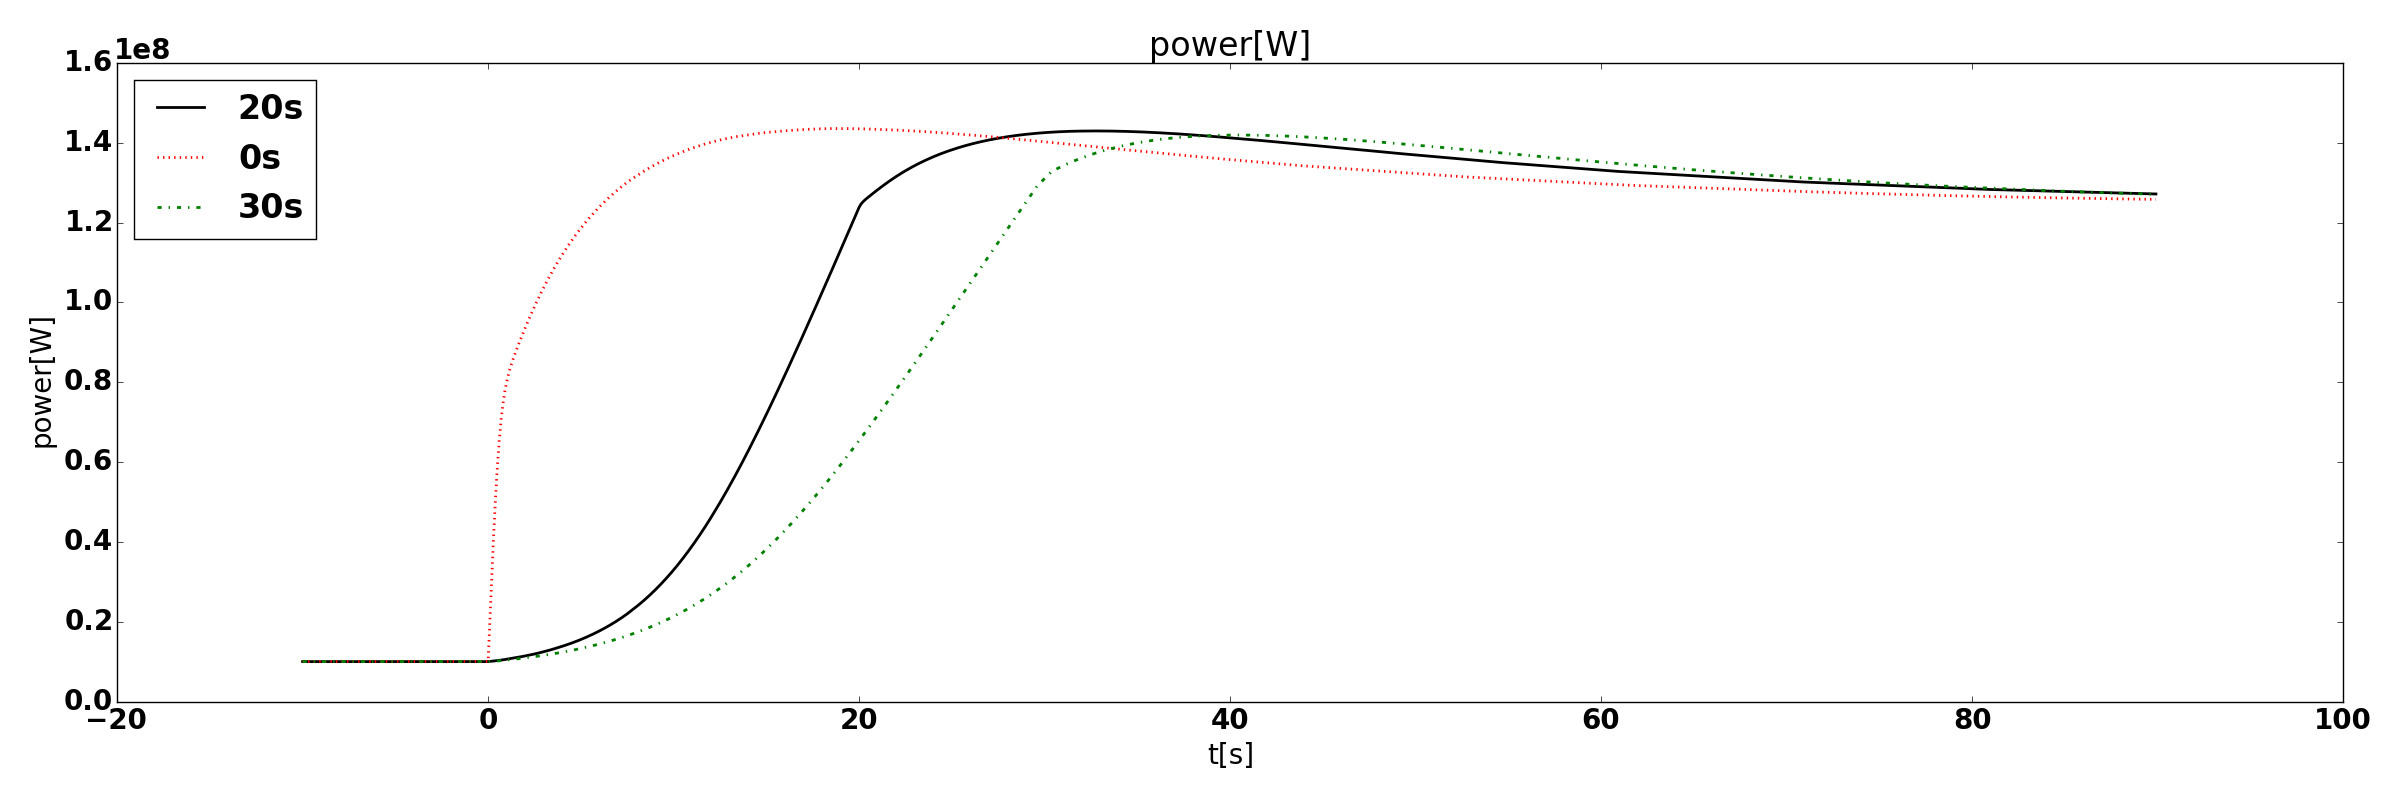
\includegraphics[width=0.55\textwidth]{diffusion/mk1/SS/power.png}
  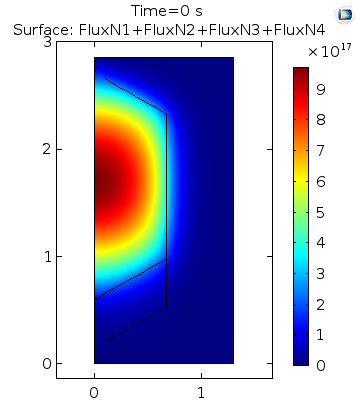
\includegraphics[width=0.49\textwidth]{diffusion/mk1/SS/fast_flux.png}
  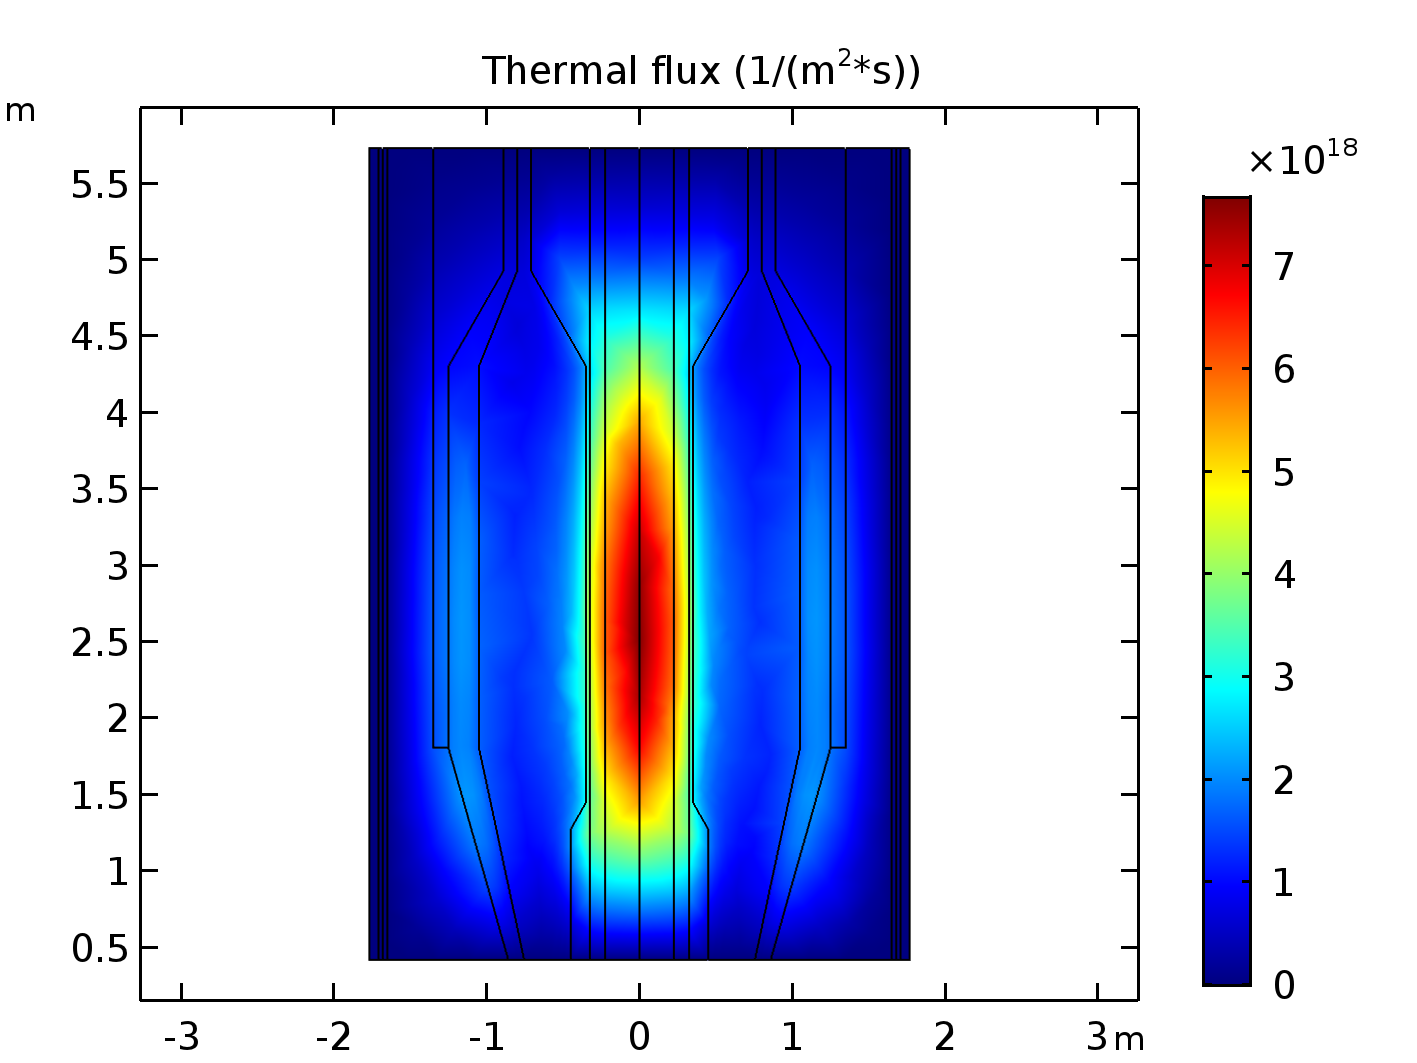
\includegraphics[width=0.49\textwidth]{diffusion/mk1/SS/thermal_flux.png}
  \caption{Steady state power and neutron flux distribution at operating conditions}
  \label{fig:mk1_flux}
\end{figure}






\subsection{Coolant flow optimization}
\label{sec:pressure}



\begin{figure}[h]
    \centering
    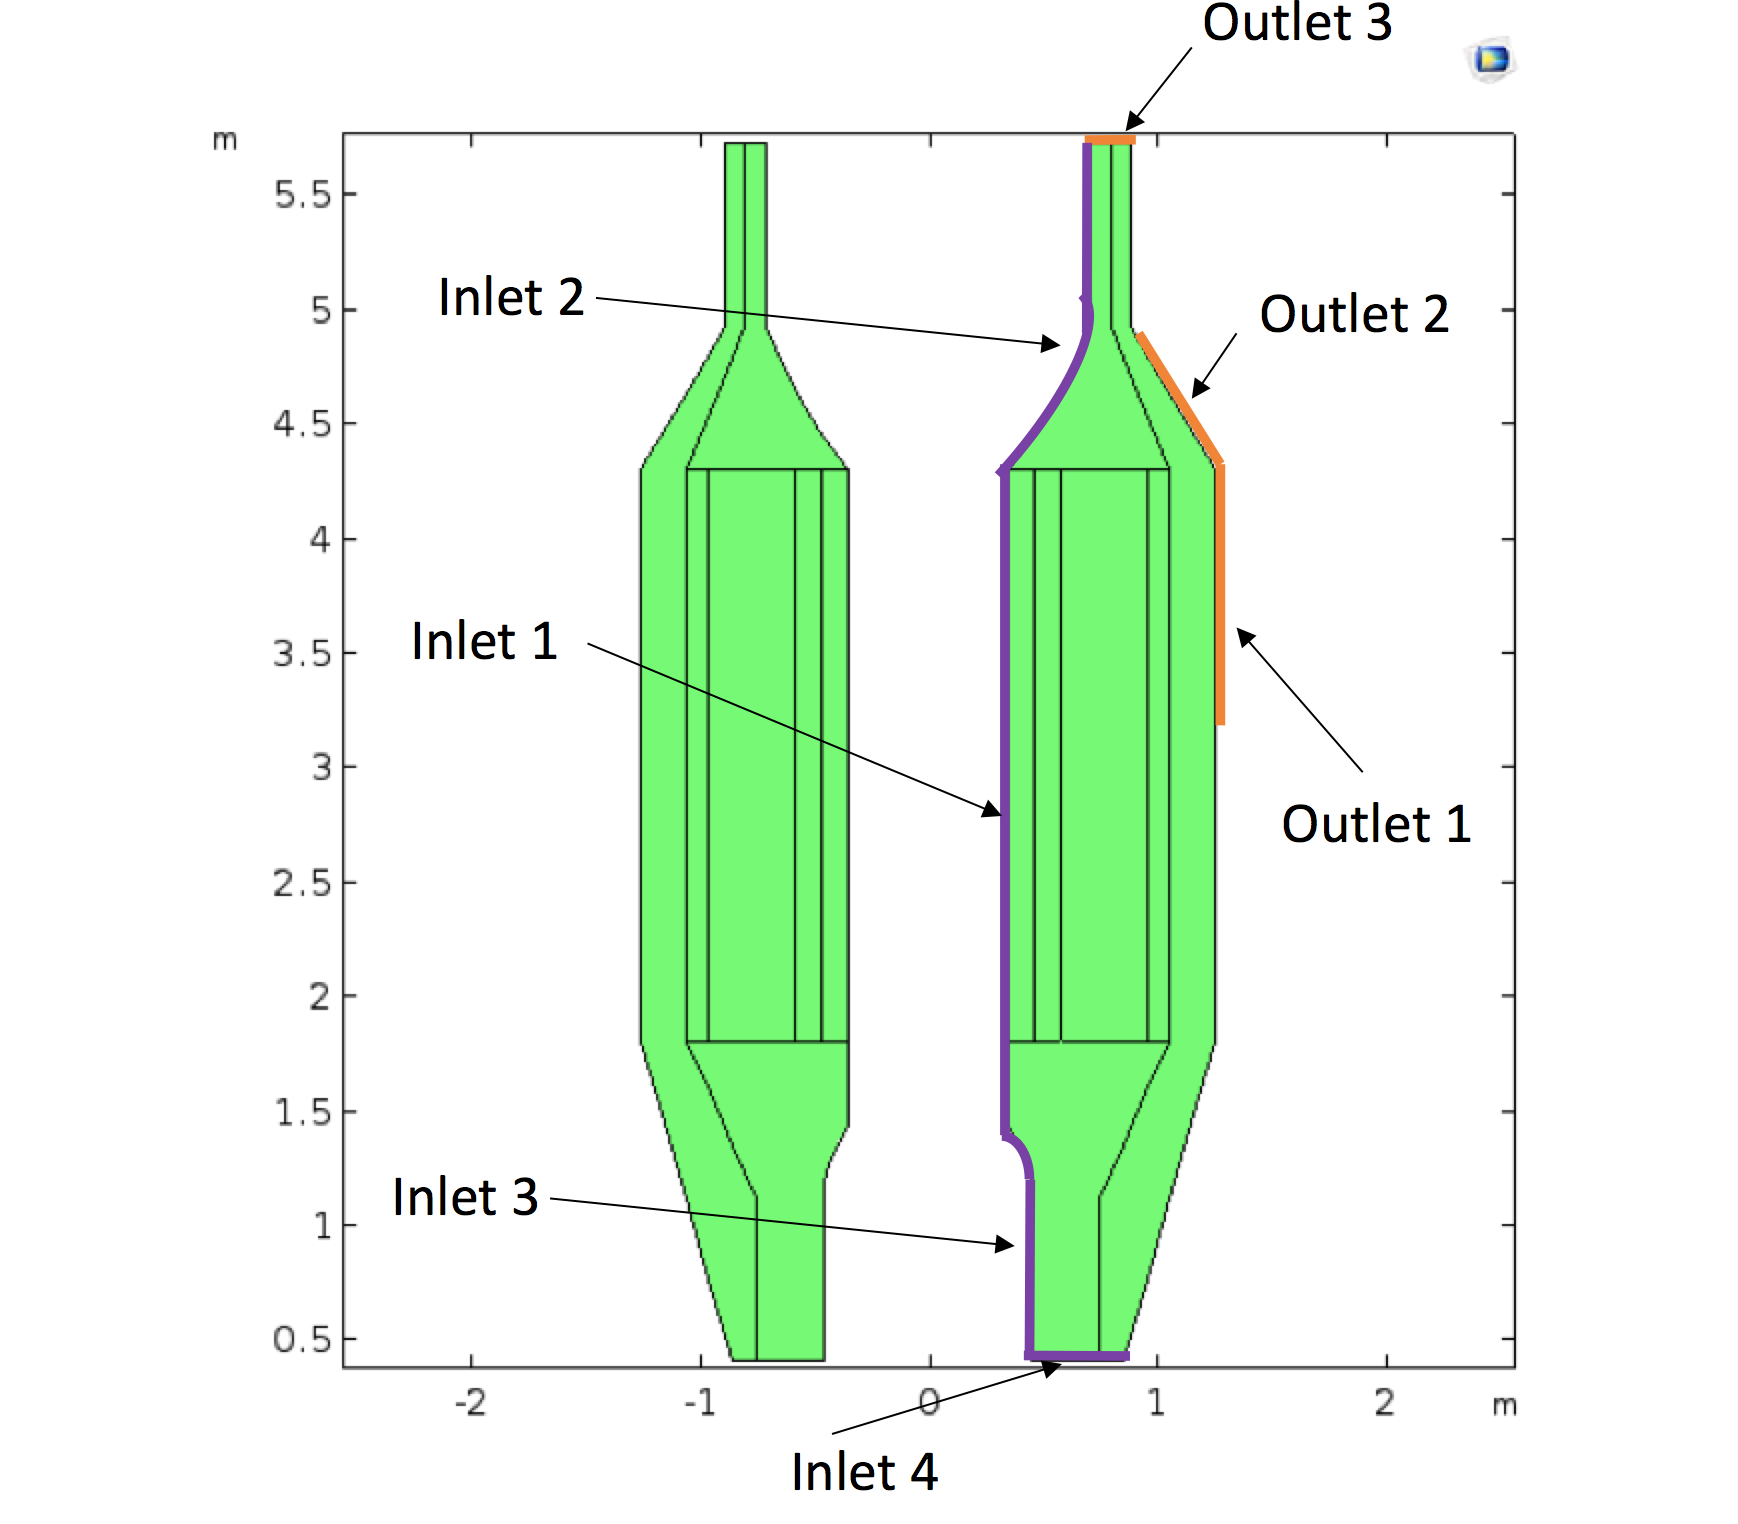
\includegraphics[width=0.7\textwidth]{images/diffusion/mk1/inlet_outlet.png}
    \caption{Schematic of Mk1 core inlet and outlet locations}
    \label{fig:inlet_outlet}
\end{figure}


\begin{figure}[h]
\centering
  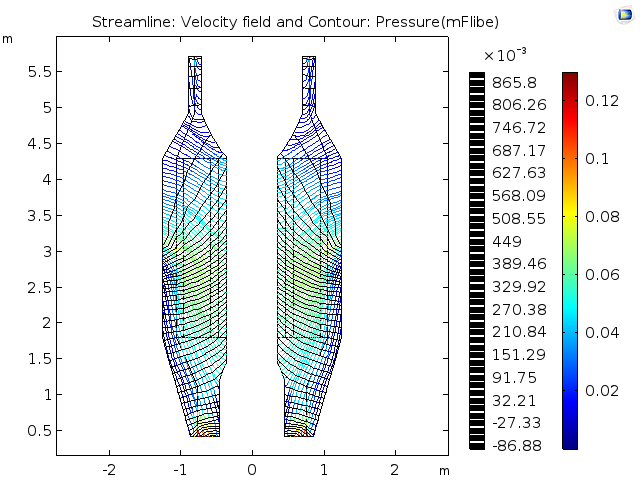
\includegraphics[width=0.9\textwidth]{diffusion/mk1/SS/flow.png}
  \caption{Steady state coolant flow streamline and pressure distribution. (Color bar legend for velocity, Isobar profile in black.)}
  \label{fig:mk1_flow}
\end{figure}

Compare to the fuel rods design in LWRs, the pebble bed geometry in the FHRs may cause higher pressure drop, which would require higher primary pump power, reduces natural circulation performance at the passive safety mode, and increases salt level swelling at free surfaces. To mitigate this shortcoming, a unique annular geometry is incorporated in the Mk1 core design. 
In addition to the bottom inlet and the top outlet that exist in most of the nuclear reactors, which result in mainly axial coolant flow with local turbulence caused by various flow mixing structures, the annular core allows inlet and outlet openings in the center and outer reflectors, as shown in figure \ref{fig:inlet_outlet} and forms cross flow pattern in the core.
The annular geometry of Mk1 provides a lot of design flexibility in terms of inlet and outlet opening locations and coolant flow boundary conditions, with the goal to achieve optimal cooling while controlling the pressure drop across the core. 


An example flow field with pressure distribution is shown in figure \ref{fig:mk1_flow}. We observe that the isobars are denser in the sections where the flow is mainly axial. This indicates that the total pressure drop across the core can be reduced by opening up the flow channels in the middle of the center and outer reflectors that enhances radial flow.
In fact, results have shown that by opening the middle inlets and outlets while keeping the pressure boundary condition fixed, the flow rate increases significantly with the inlet and outlet widths. In the range that is studied, opening either outlet or inlet has similar effect on the flow rate, about 62~kg/s increase with 1cm increase of outlet or 54~kg/s with 1~cm of inlet. With this trend, it is feasible to keep the pressure drop at 1~m head loss with reasonable opening width. 

Another important parameter to consider during optimization is the temperature as the primary function of coolant is to transport the heat from the fuel elements to the primary loop and ultimately to the secondary loop and beyond for power conversion. The flow pattern directly affects the local heat transfer properties, represented in the models by the convective heat transfer coefficient.   
Therefore one goal for flow optimization is to keep the peak fuel and coolant temperatures below their respective safety limits. 

The nominal average fuel temperature in a Mk1 core is much lower than the safety limit due to the excellent thermal resistance of the TRISO type fuel. 
Although the fuel elements in FHRs are highly thermal resistant so that the peak fuel temperature is not the primary concern in a FHR core, the fuel temperature as a safety design criteria needs to be monitored in all events. The fuel temperature is determined by three factors, the power density, the local coolant temperature, and the particle to fluid heat transfer coefficient. Begin able to bring cold coolant up in the channels in the center reflector and inject to higher locations where the fuel is hot is a unique heat transfer enhancement design advantage in the Mk1 FHR core. The particle-to-coolant heat transfer coefficient in a pebble bed core is dictated by the Prandtl number, an inherent properties of the salt, and the Reynolds number, which is a dimensionless number that characterizes the flow regime. Figure \ref{fig:h_conv} shows the heat transfer coefficient distribution side-by-side with the Reynolds number. Only limited heat transfer occurs between the solid fuel element and the coolant where the Reynolds number approaches zero.
Therefore, avoiding local hot spot in fuel temperature, which can be a result of dead-zones in the flow is the key in flow optimization with respect to peak fuel temperature. 


\begin{figure}
\centering
  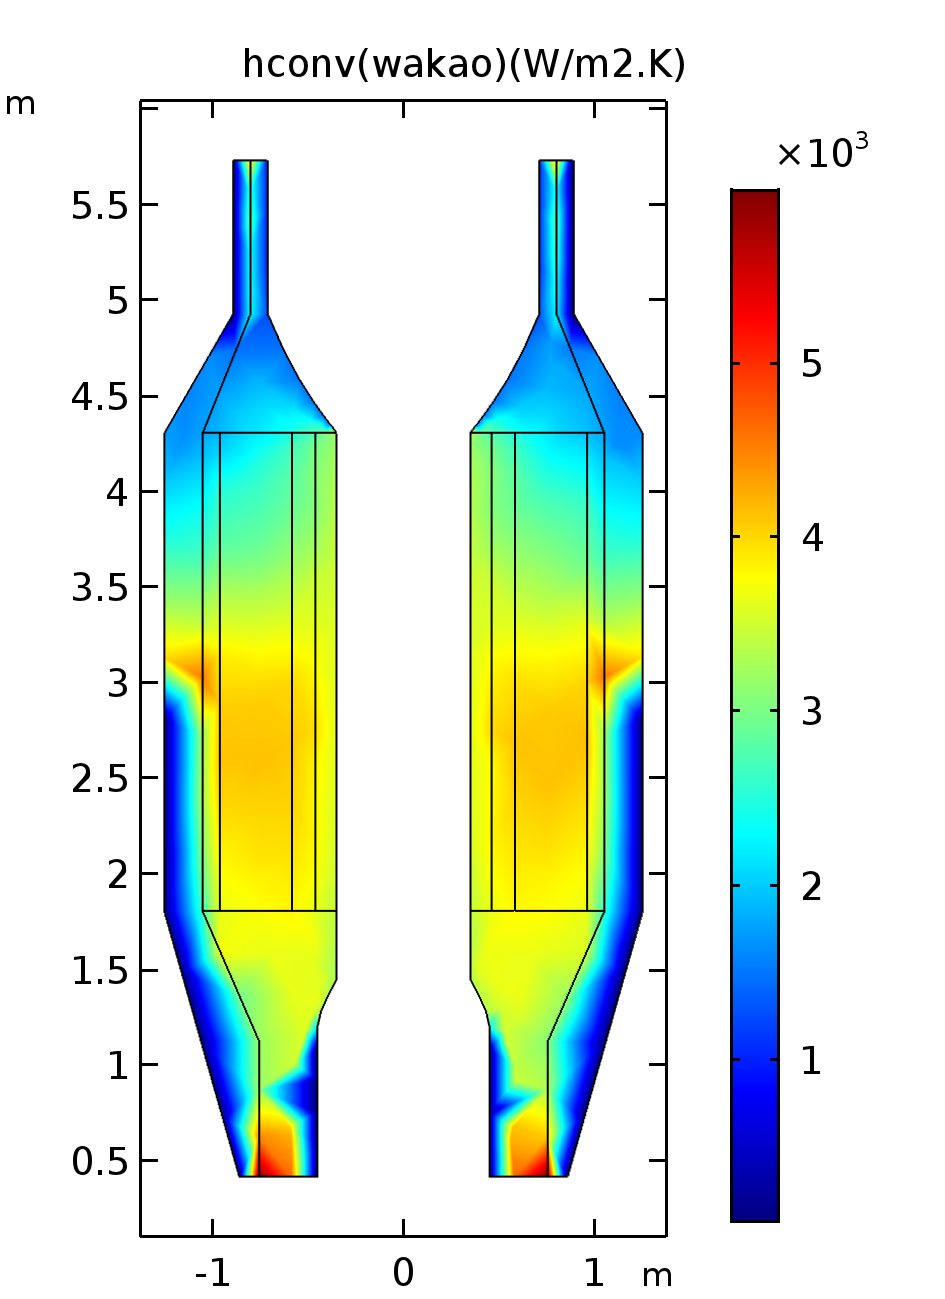
\includegraphics[width=0.46\textwidth]{diffusion/mk1/SS/h_conv.png}
  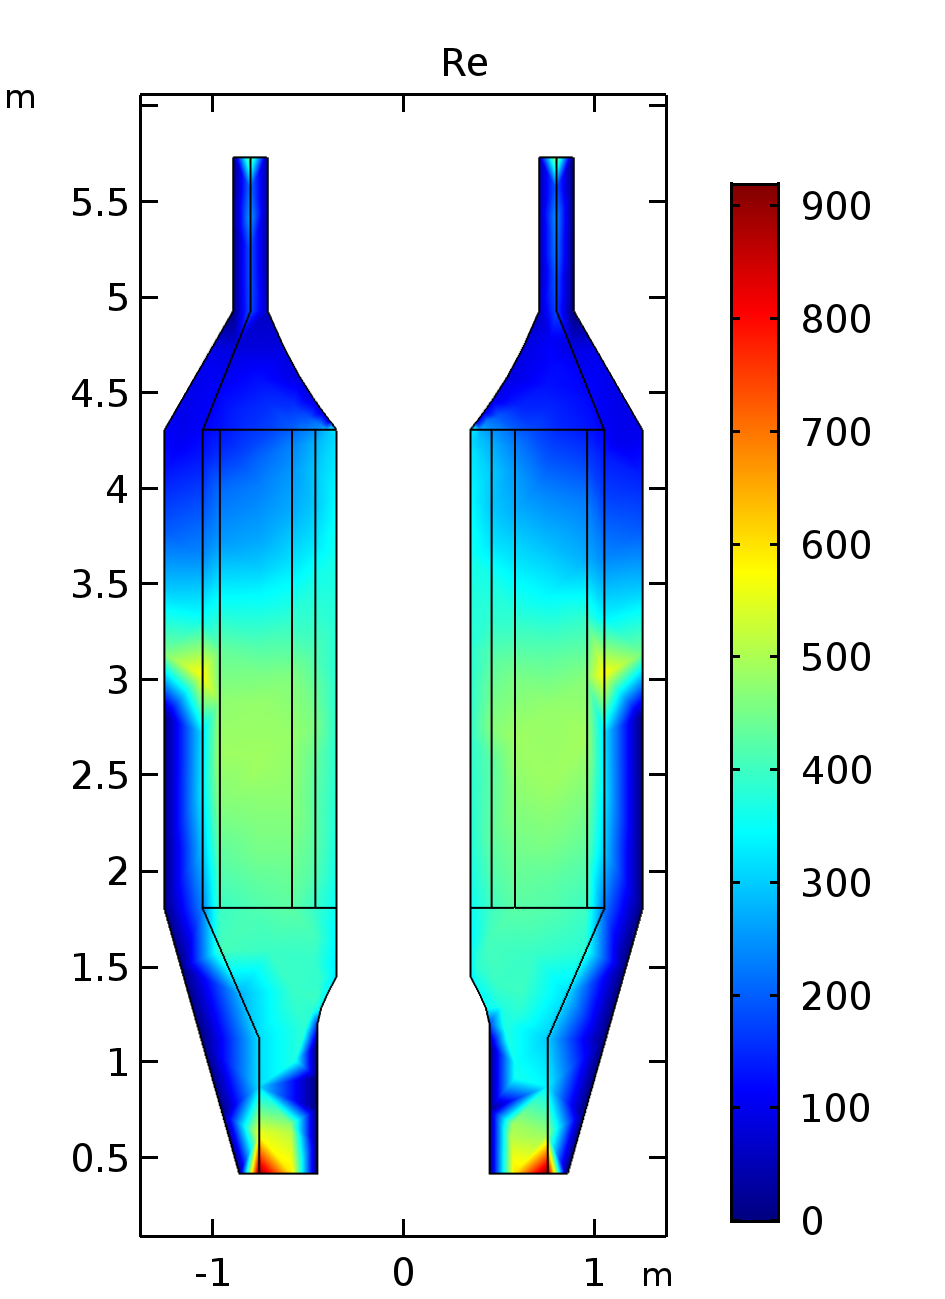
\includegraphics[width=0.46\textwidth]{diffusion/mk1/SS/Re.png}
  \caption{Steady state local convective heat transfer coefficient, computed from Wakao correlation, and the Reynolds number}
  \label{fig:h_conv}
\end{figure}

The peak coolant temperature in the core is also important to damage to metallic structures in the outlet plenum and to prevent boiling, although boiling is not the limiting design criteria for Mk1 as the coolant in Mk1 has very high boiling point. At nominal operating condition, 976 kg coolant enters the core every second at 600 \degc\ and the bulk average outlet coolant temperature is 713 \degc\, much lower than the flibe boiling point at atmospheric pressure.
In terms of temperature limit, the smallest thermal margin in the core is in the coolant outlet temperature, because the outlet coolant temperature directly affects the hot leg metallic structures, which is more vulnerable to thermal degradation than the fuel elements and graphite blocks in the core. 
In addition to the average outlet temperatures, the uniformity of the  outlet coolant temperature is also important to extend the lifetime of the structural material at the exit of the core. Turbulent mixing of the coolant in the upper plenum is often incomplete, causing temperature fluctuation and gradient in the hot leg of the main circulation pipe that can cause thermal fatigue. 

 The spread in coolant temperature around the average can be controlled by careful design of the inlet coolant velocity profile that achieves a similar temperature increase along all the streamlines.

To study the effects of inlet boundary condition on the temperature criteria, we have tested three different inlet velocity profiles. The inlet velocity profile at the center reflector is shown in \ref{fig:inlet_vel}. All these have 70\% of the total inlet routed through the center reflector and 30\% from the bottom inlet (not shown in the figure). 
To achieve the flexibility in fine-tuning the inlet injection design, a parabolic function is used to model the main center inlet (inlet 1 in figure \ref{fig:inlet_outlet}). The first one allows coolant injection at only limited heights.
The second one is optimized for cooling efficiency, where the coolant injection is more evenly distributed with the highest flow rate near the middle of the core where the flow path between inlet and outlet is the longest and the power density is the highest, for better cooling efficiency.
However, in practice, the ability to bring the coolant flow up to the top is limited by the cross-sections area of the flow channels in the center reflector. Thus, a bottom heavy inlet condition is more realistic. 



\begin{figure}
    \centering
    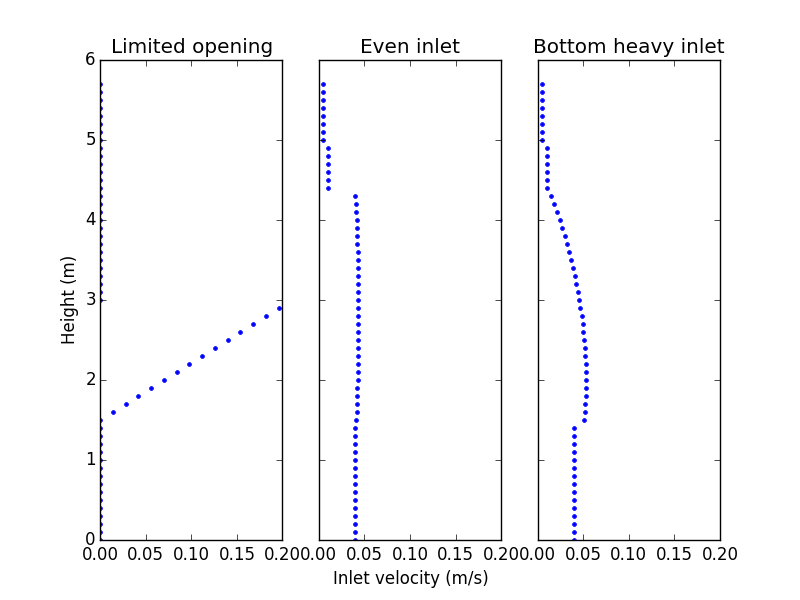
\includegraphics[width=0.8\textwidth]{images/diffusion/mk1/SS/flow_opti/inlet_vel.png}
    \caption{Center reflector coolant injection velocity boundary condition}
    \label{fig:inlet_vel}
\end{figure}

Figure \ref{fig:mk1_temp_flibe} shows the temperature of the coolant as it flows through the core.
Figure \ref{fig:mk1_temp_fuel} shows TRISO kernel temperature distribution in the core.
And histograms in figure \ref{fig:hist_flibe} show the distribution of outlet coolant temperature under the different inlet conditions.
With limited opening in the middle, there is a large variation in the coolant outlet temperature.
In particular, the top of the core is overheated due to limited coolant flow in that area, where the inlet is closed.
In the contrary, with improved inlet design, the coolant can efficiently cover all the areas in the core and provide sufficient cooling to the fuel. 
Although the power peaks at the center (figure \ref{fig:mk1_full_power}), the fuel and the coolant temperatures are low in the center because of the inlet coolant along the center reflector. The peak temperature for both phase is found near the outlet.
Under the bottom heavy inlet condition, most of the coolant exits the core with a temperature between 680 \degc\ and 720 \degc\ . And peak outlet coolant are below 770 \degc, this allows a thermal margin to structural material damage.





\begin{figure}
\centering
    \begin{subfigure}[b]{0.42\textwidth}
        \centering
         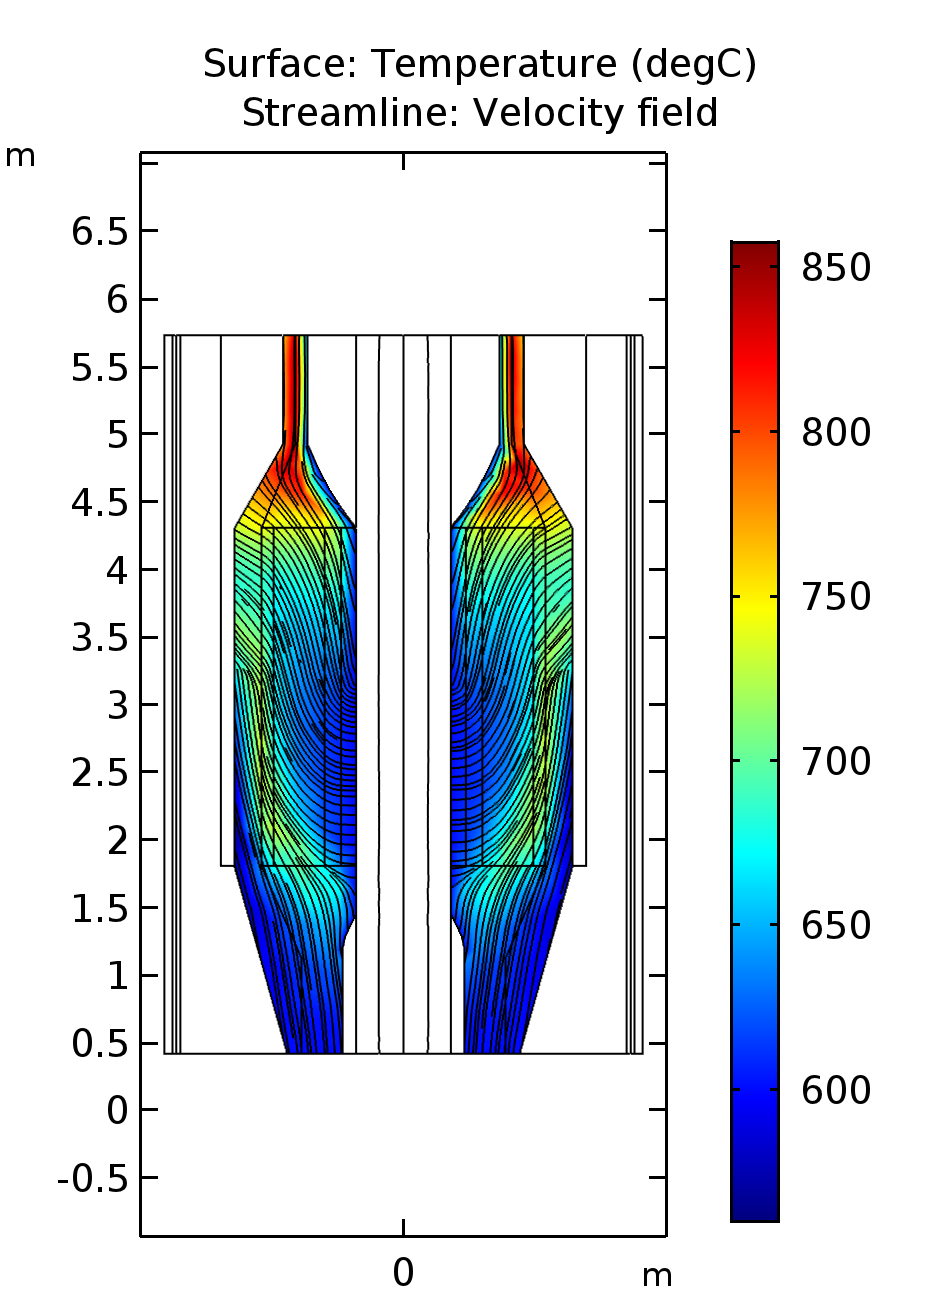
\includegraphics[width=\textwidth]{images/diffusion/mk1/SS/flow_opti/T_flibe_init.png}
        \caption{Limited opening}
    \end{subfigure}%
    ~ 
    \begin{subfigure}[b]{0.42\textwidth}
        \centering
        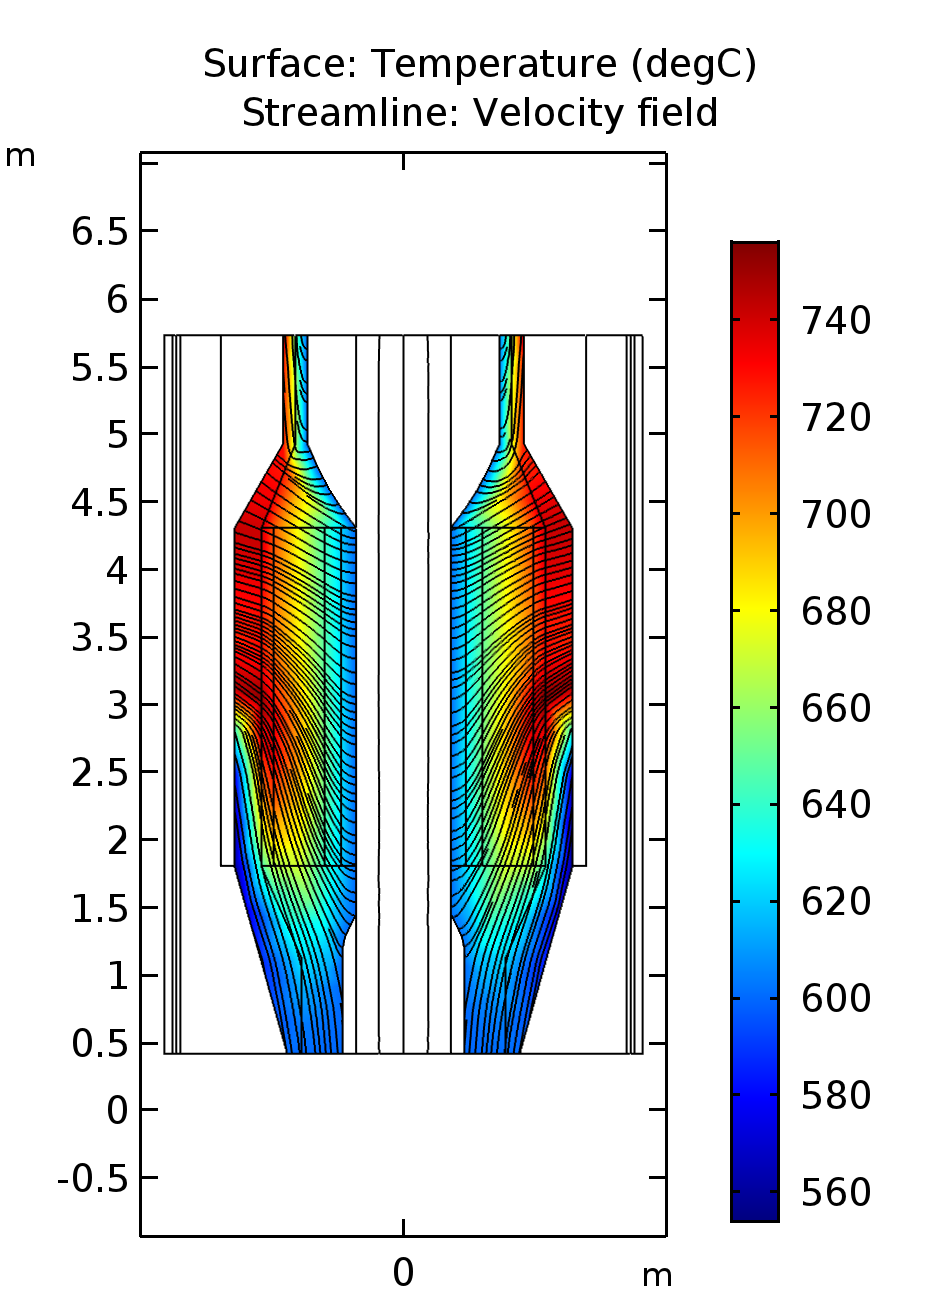
\includegraphics[width=\textwidth]{images/diffusion/mk1/SS/flow_opti/T_flibe_even1.png}
        \caption{Even inlet}
    \end{subfigure}
  
    \begin{subfigure}[b]{0.45\textwidth}
        \centering
        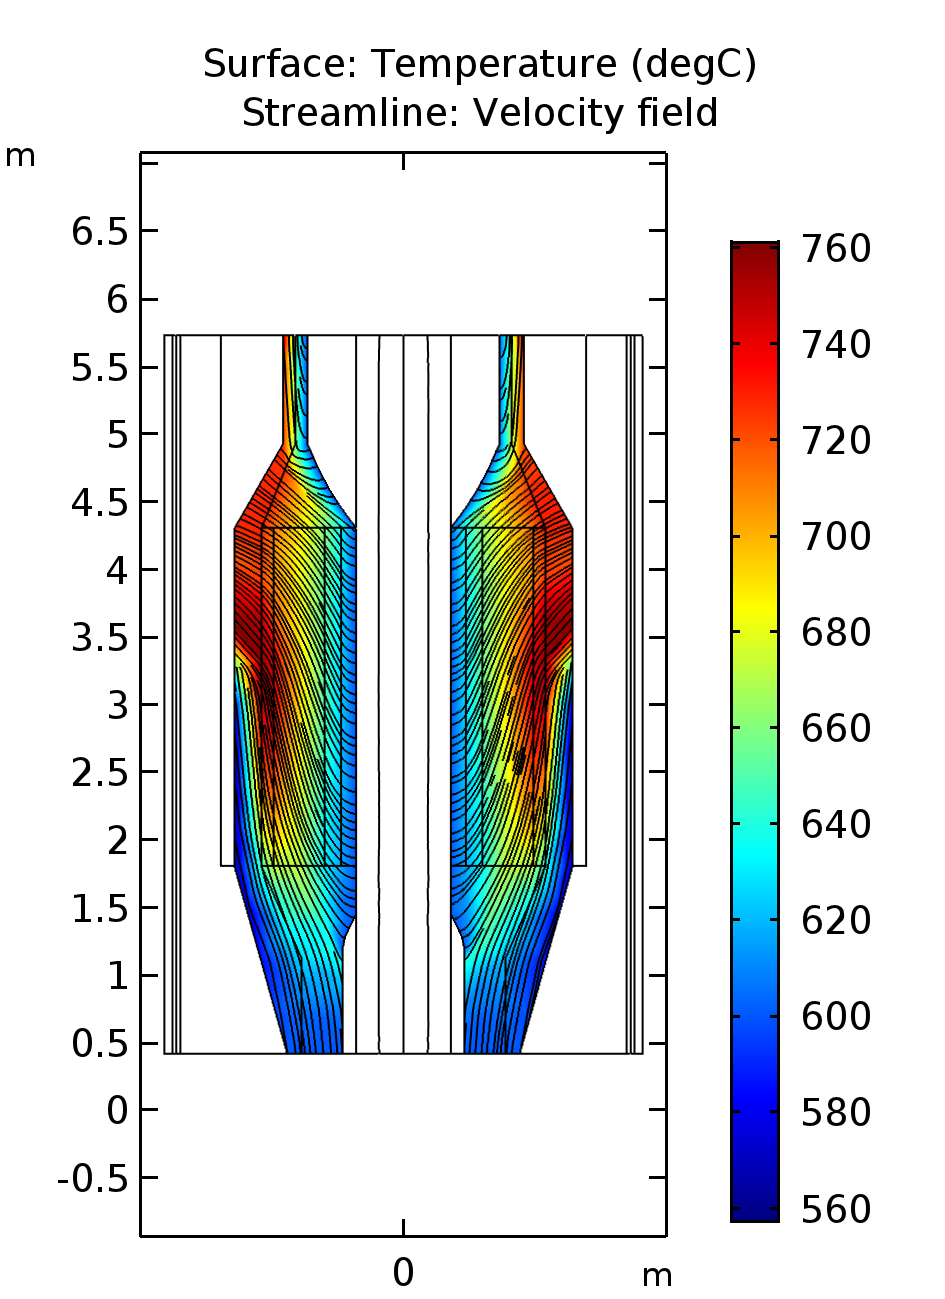
\includegraphics[width=\textwidth]{images/diffusion/mk1/SS/flow_opti/T_flibe_bottom.png}
        \caption{Bottom heavy inlet}
    \end{subfigure}

    \caption{Steady state coolant temperature distribution and streamline under different inlet conditions}
    \label{fig:mk1_temp_flibe}
\end{figure}

\begin{figure}
\centering
      \begin{subfigure}[b]{0.42\textwidth}
        \centering
         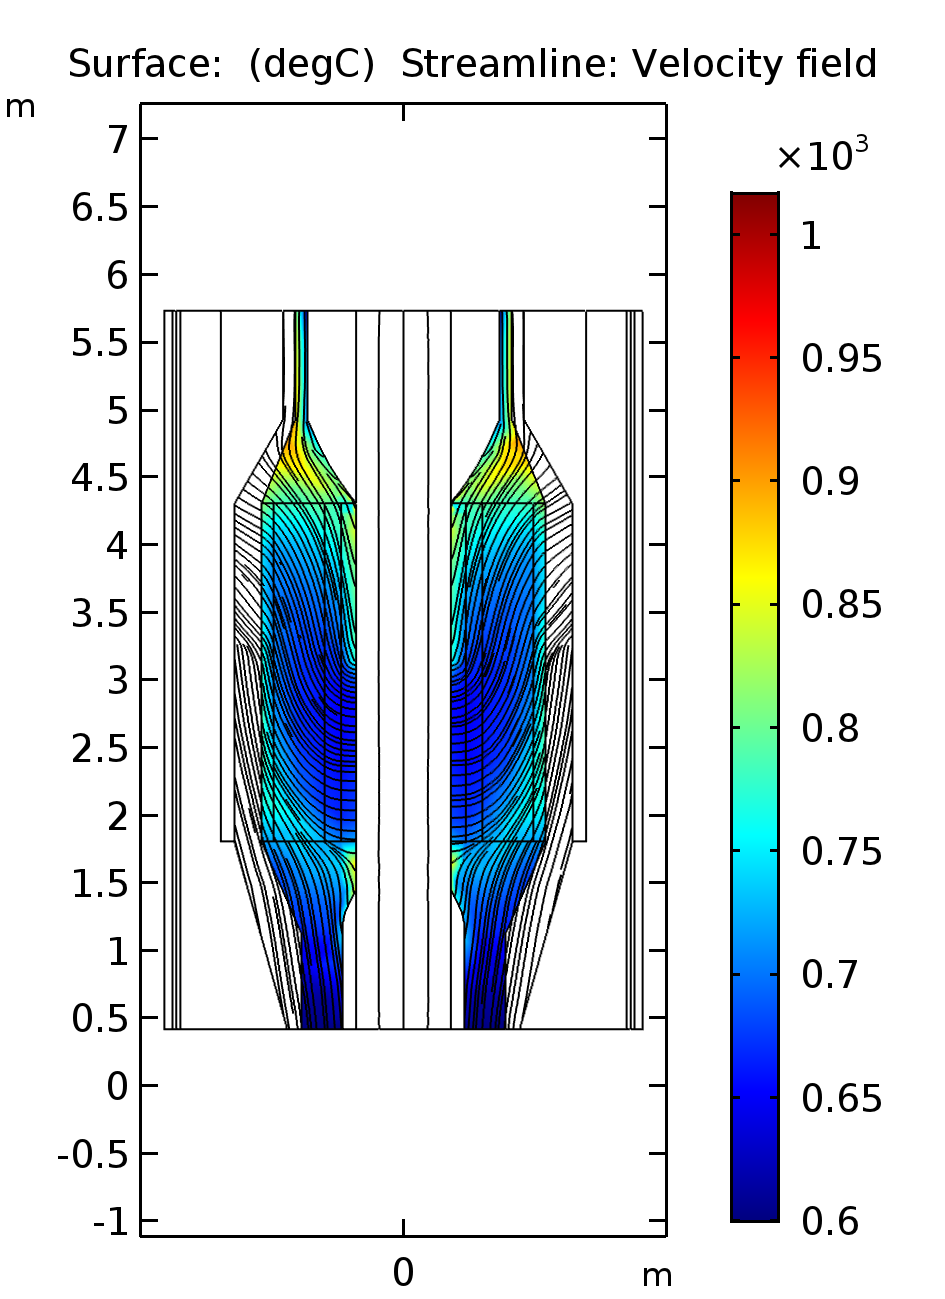
\includegraphics[width=\textwidth]{images/diffusion/mk1/SS/flow_opti/T_fuel_init.png}
        \caption{Limited opening}
    \end{subfigure}%
    ~ 
    \begin{subfigure}[b]{0.42\textwidth}
        \centering
        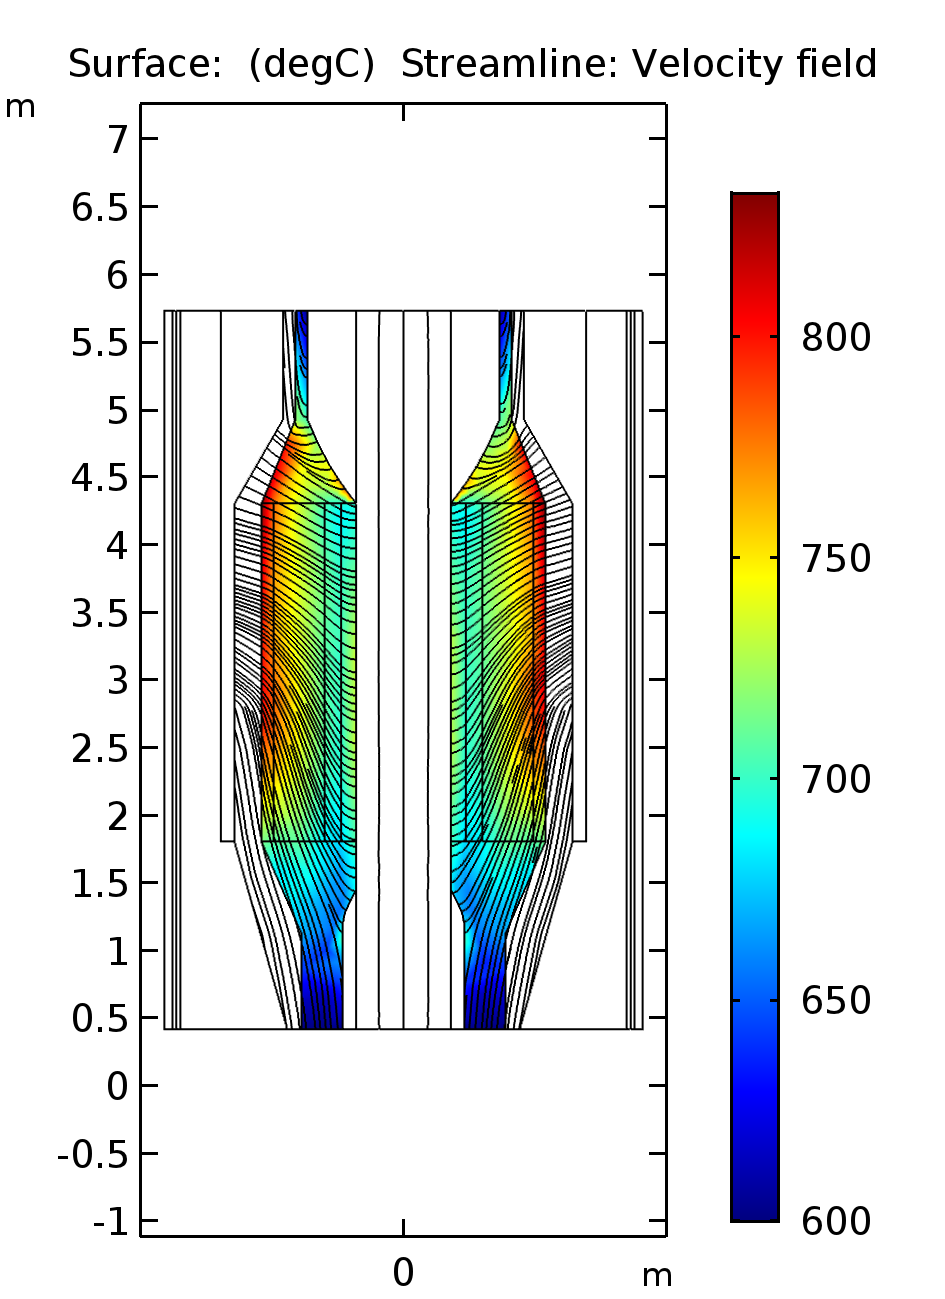
\includegraphics[width=\textwidth]{images/diffusion/mk1/SS/flow_opti/T_fuel_even_1.png}
        \caption{Even inlet}
    \end{subfigure}
  
    \begin{subfigure}[b]{0.45\textwidth}
        \centering
        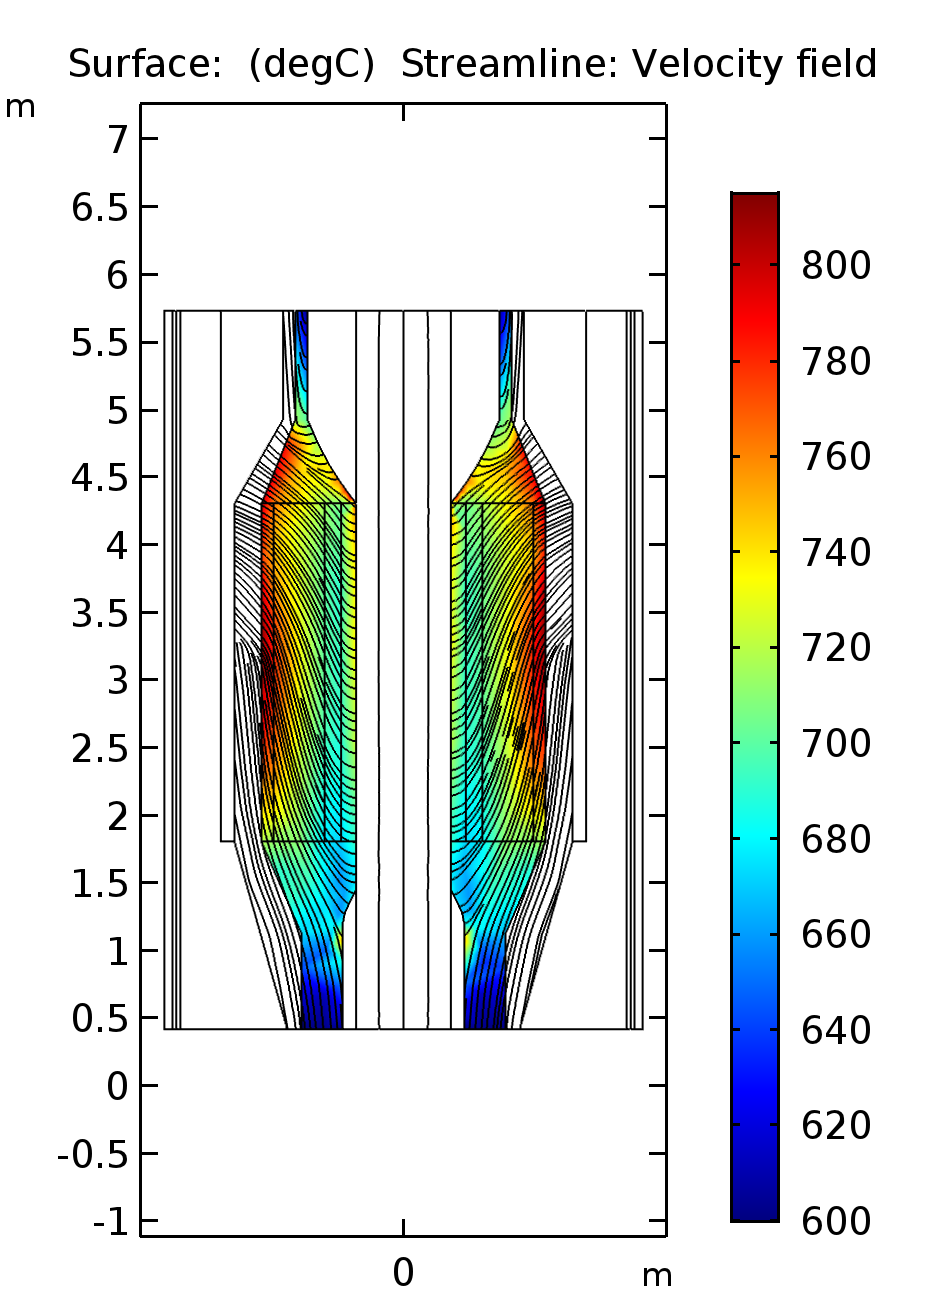
\includegraphics[width=\textwidth]{images/diffusion/mk1/SS/flow_opti/T_fuel_bottom.png}
        \caption{Bottom heavy inlet}
    \end{subfigure}
  
  \caption{Steady state fuel temperature distribution and streamline}
  \label{fig:mk1_temp_fuel}
\end{figure}

\begin{figure}
    \centering
    \begin{subfigure}[b]{0.42\textwidth}
    \centering
     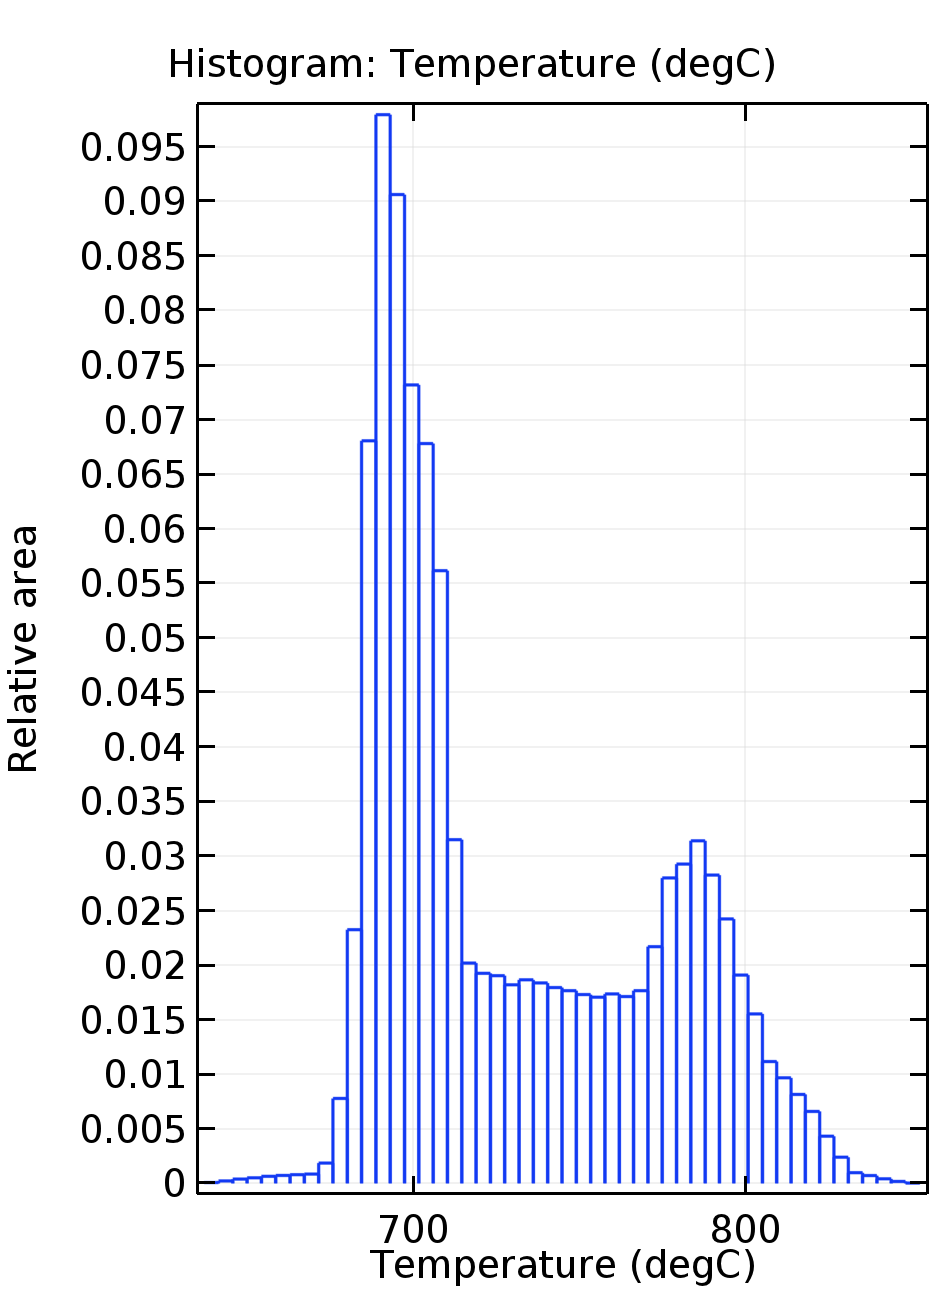
\includegraphics[width=\textwidth]{images/diffusion/mk1/SS/flow_opti/hist_init.png}
    \caption{Limited opening}
    \end{subfigure}%
    ~ 
    \begin{subfigure}[b]{0.42\textwidth}
        \centering
        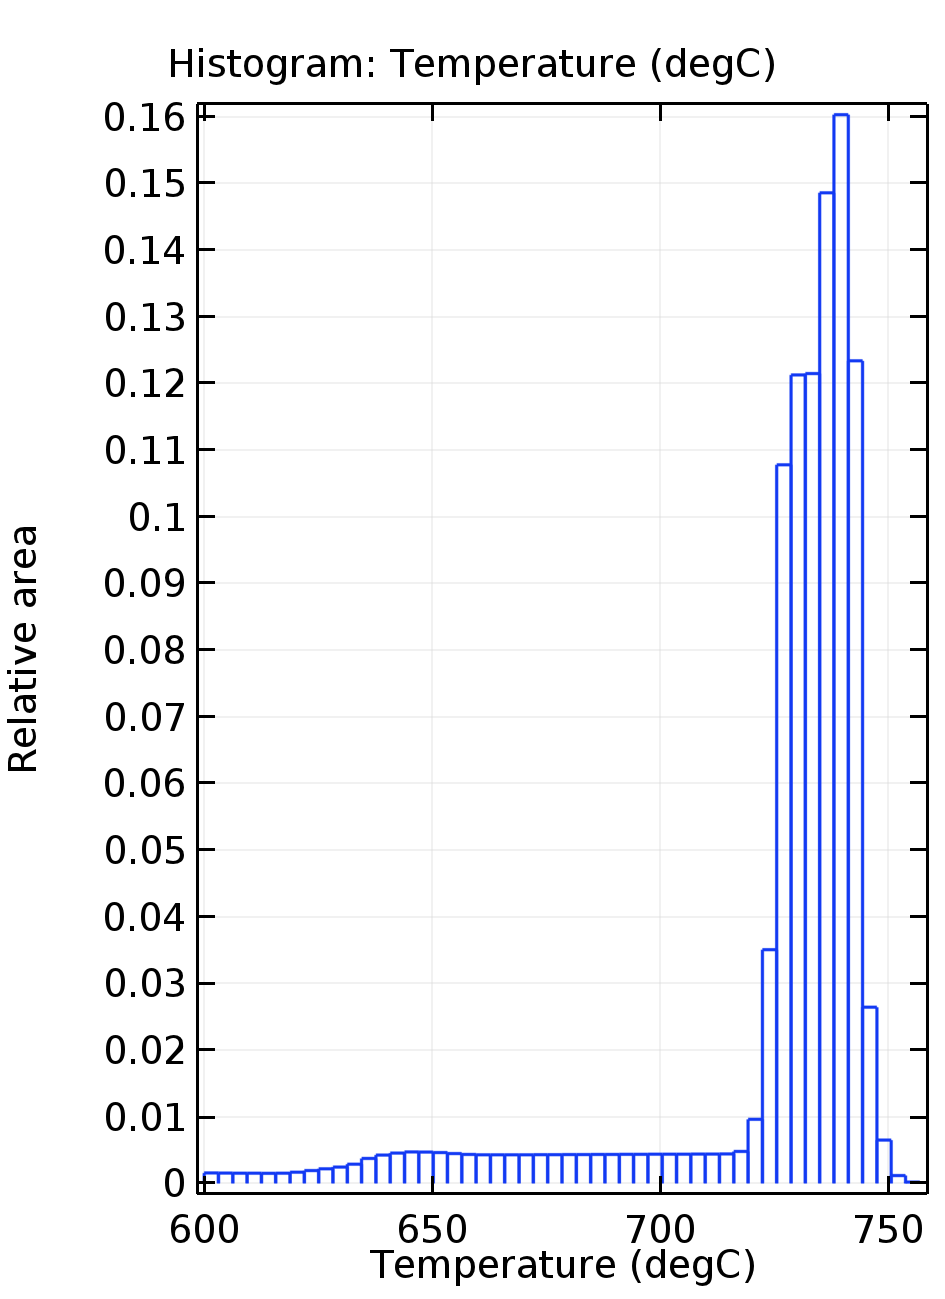
\includegraphics[width=\textwidth]{images/diffusion/mk1/SS/flow_opti/hist_even.png}
        \caption{Even inlet}
    \end{subfigure}

    \begin{subfigure}[b]{0.45\textwidth}
    \centering
    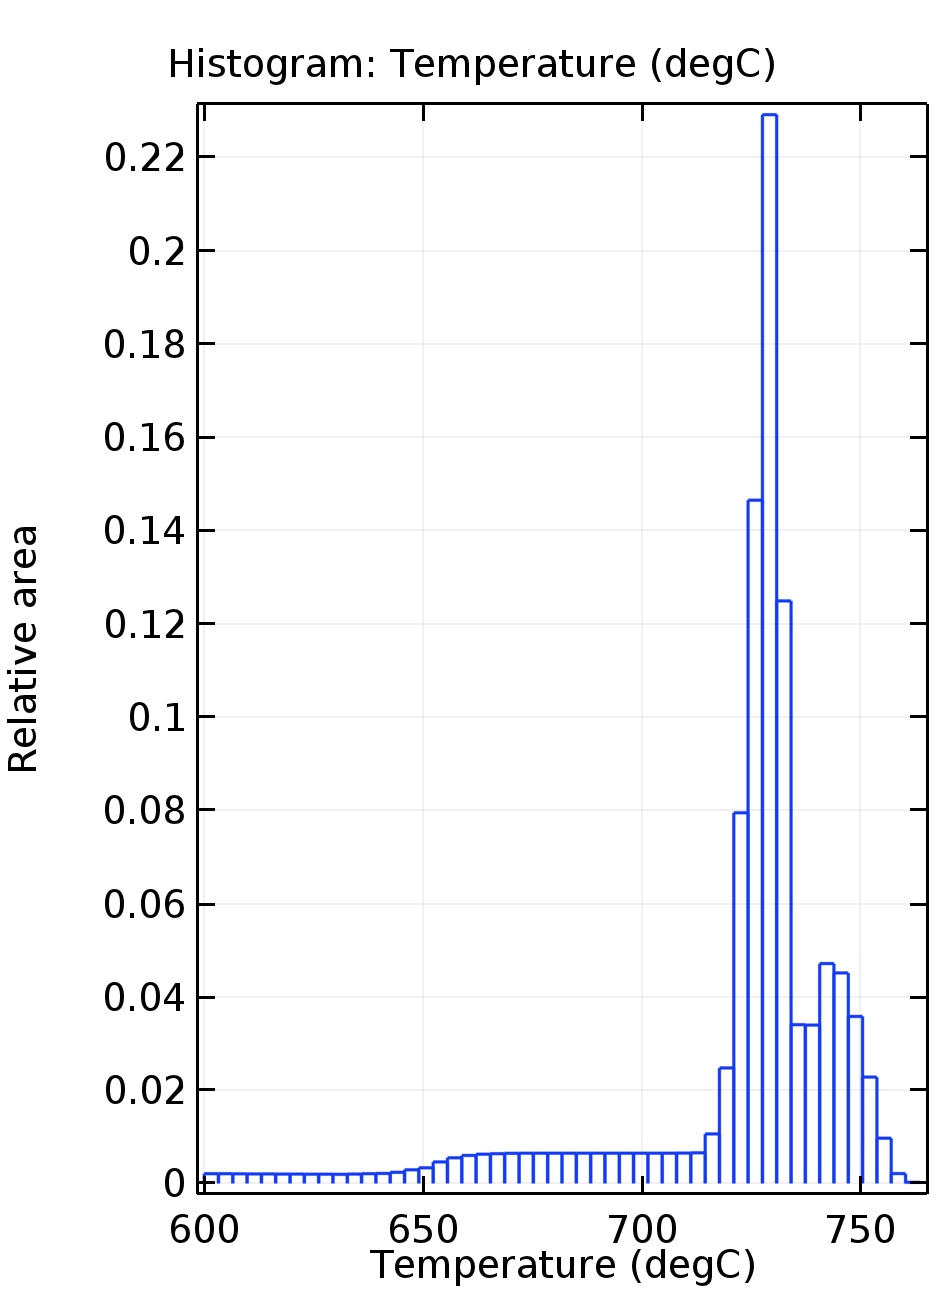
\includegraphics[width=\textwidth]{images/diffusion/mk1/SS/flow_opti/hist_bottom.png}
    \caption{Bottom heavy inlet}
    \end{subfigure}
    
    \caption{Histogram of coolant outlet temperature (weighted by the surface area)}
    \label{fig:hist_flibe}
\end{figure}




 
 








% \section{Temperature reactivity feedback coefficients}
% An important parameter for transient simulation is the reactivity feedback coefficients for fuel and flibe.

% Temperature reactivity feedback coefficients are computed with equilibrium fuel composition, at nominal conditions. Uniform temperatures are assigned to the fuel and coolant to compute the variation in reactivity due to temperatures.





\newpage
\section{Transient results}
\label{sec:mk1_trans}

The coupled thermal-hydraulics and neutronics model (\ref{sec:comsol_mk1}) can be used to simulate 3 dimensional transient scenarios that does not alter the power conversion system. To demonstrate this capability, two classes of transient scenarios are simulated here, including  over-cooling transients and reactivity insertion (RI) transients.





\subsection{Overcooling transients}




An over-cooling transient happens when colder coolant introduces positive reactivity to the core via temperature reactivity feedback and causes power to increase (shown in figure \ref{fig:mk1_oc_power}). In this study, a 100$^{\circ}C$ drop in coolant inlet temperature in 10 seconds in a core with fresh fuel and without inserted control rods is simulated as an example case. 


The change in fuel temperature is determined by local power level, which is increased, and coolant temperature, which might increase due to the higher power level or decrease due to the colder inlet. Figure \ref{fig:mk1_oc_fuel} shows the core-wise peak fuel temperature. It decreases slightly at the begining and increase to almost 1150 \degc. 




\begin{figure}
    \centering
    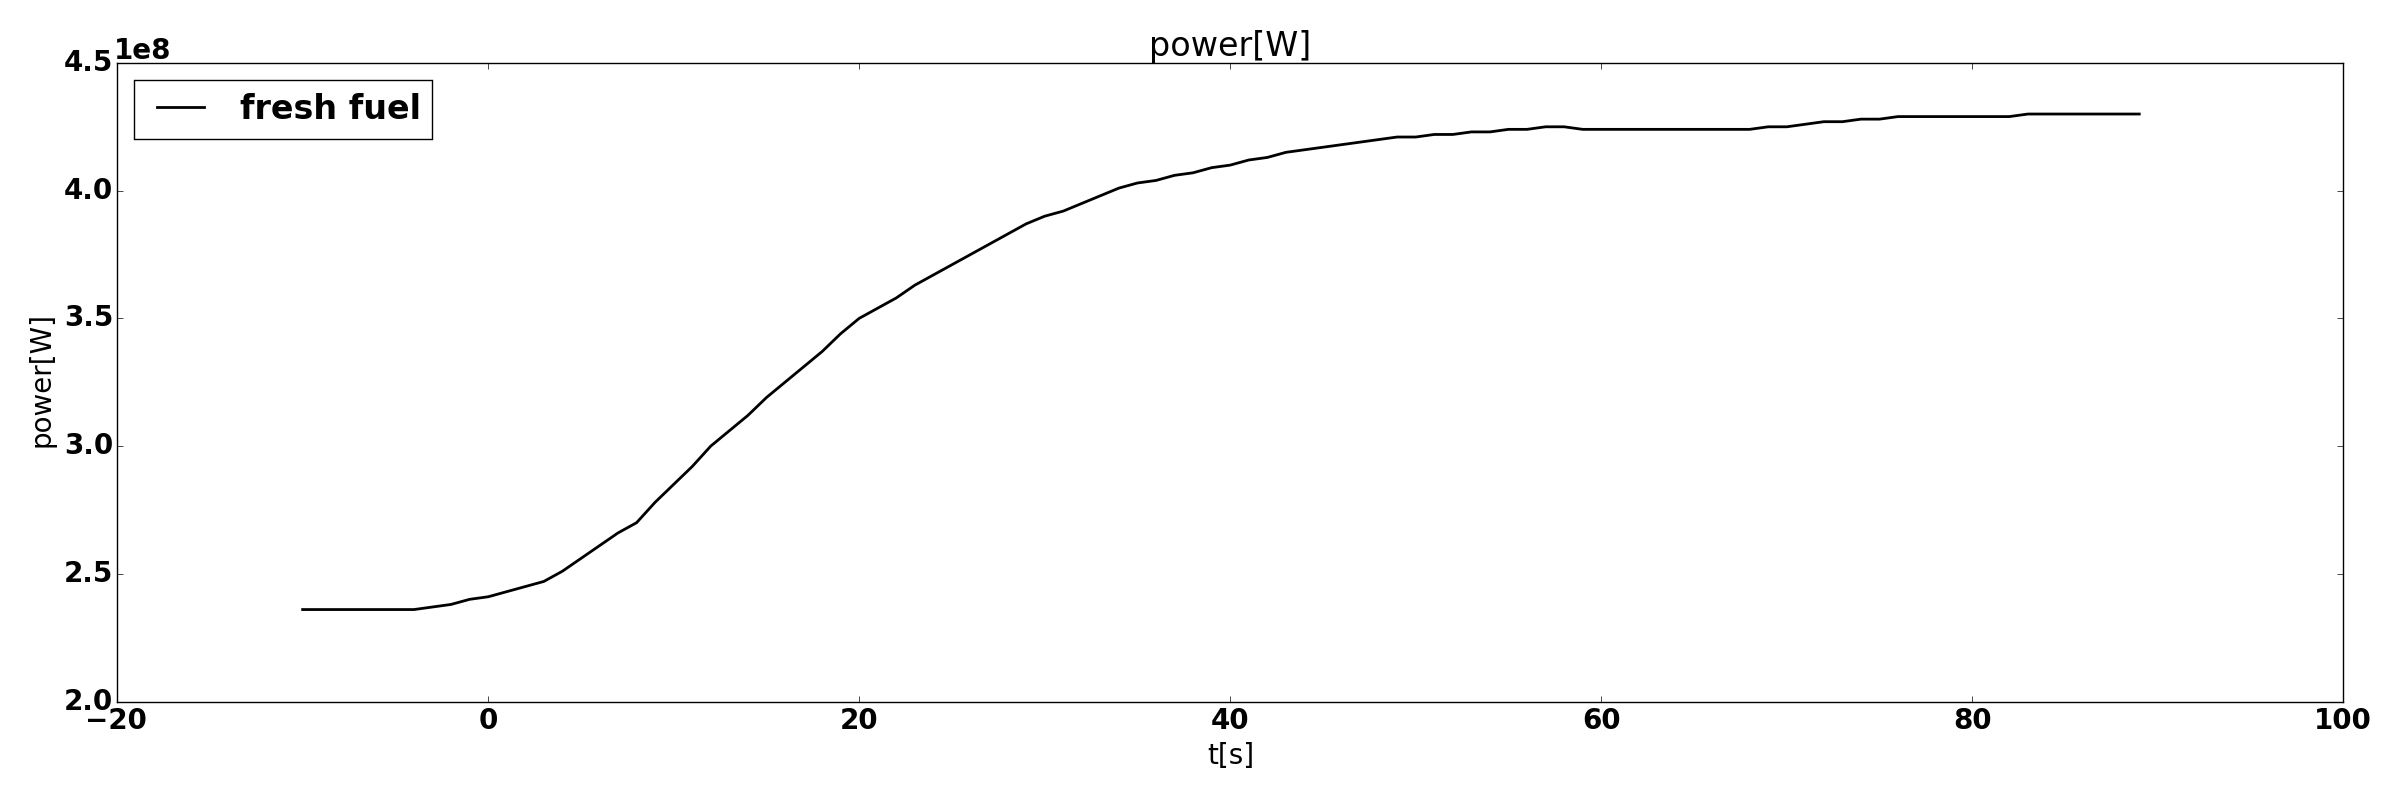
\includegraphics[width=\textwidth]{images/diffusion/mk1/OC/power.png}
    \caption{Full core power level during an overcooling transient}
    \label{fig:mk1_oc_power}
\end{figure}

\begin{figure}
    \centering
    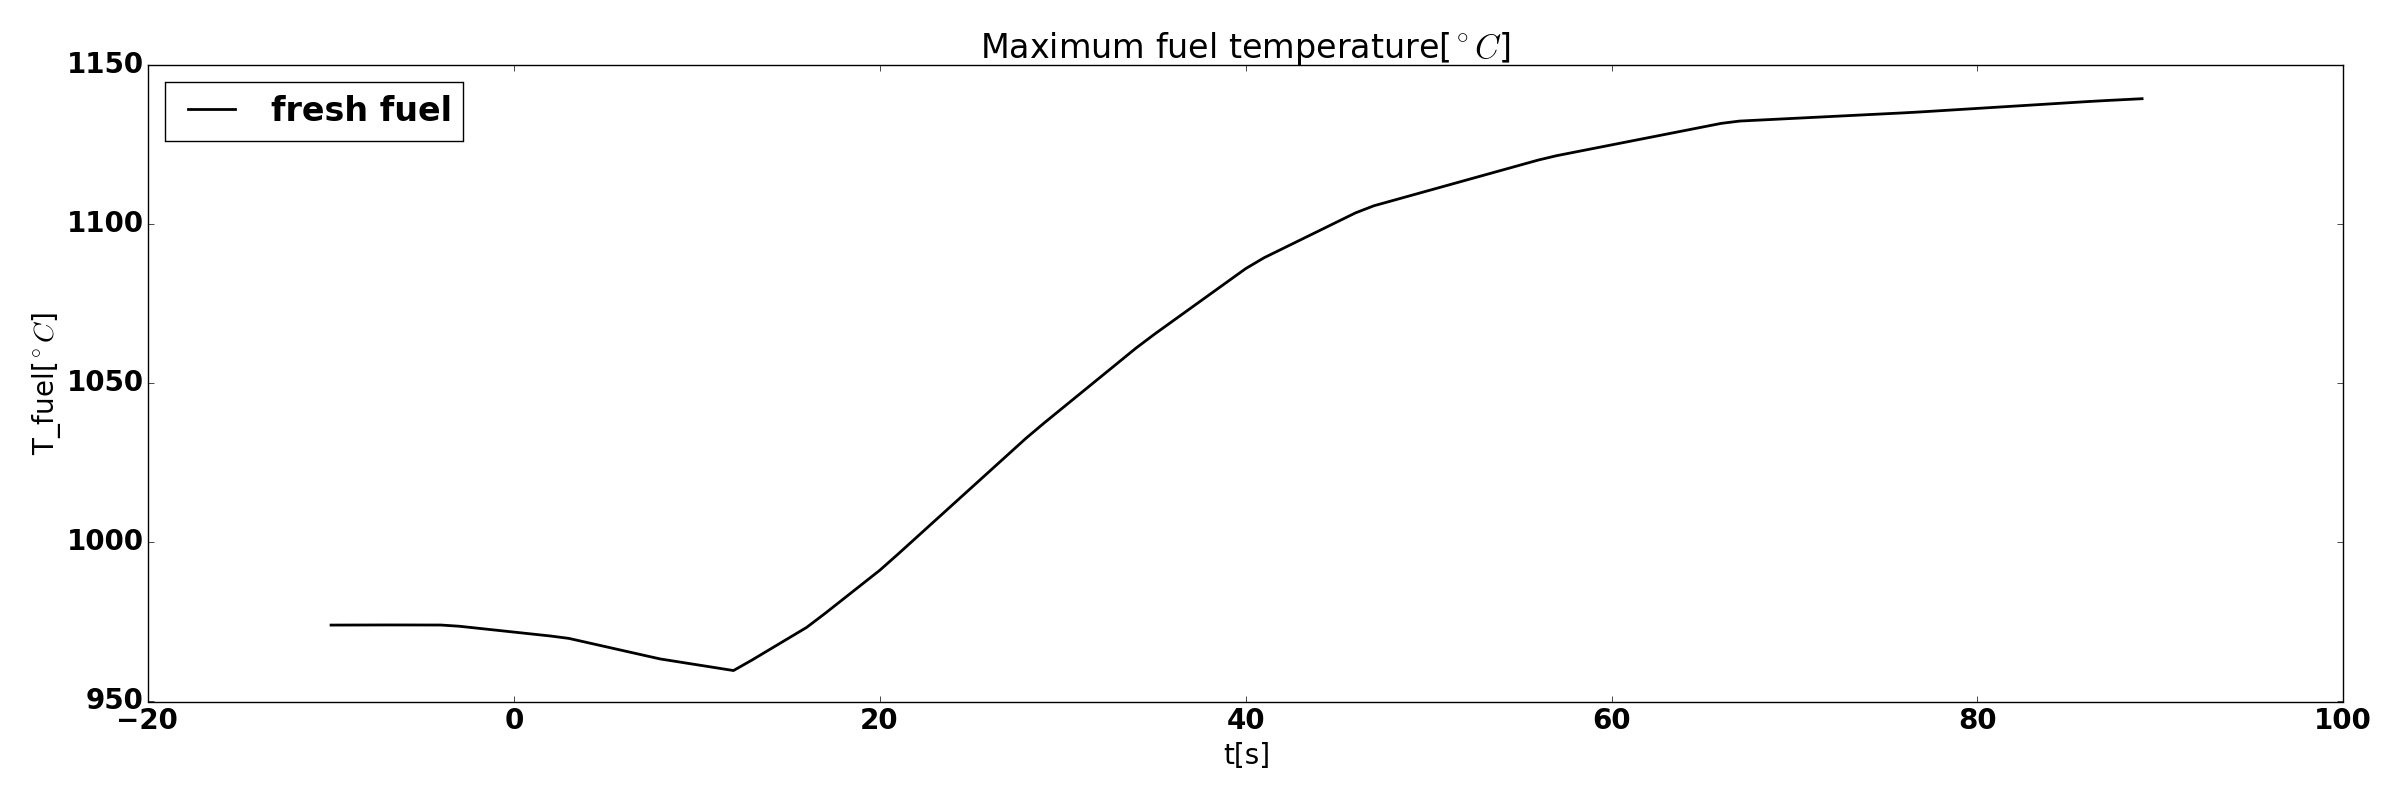
\includegraphics[width=\textwidth]{images/diffusion/mk1/OC/T_fuel_max.png}
    \caption{Maximum fuel temperature during an overcooling transient}
    \label{fig:mk1_oc_fuel}
\end{figure}

The coolant outlet temperature is shown in figure \ref{fig:mk1_oc_t_out}. It remains constant until the changes propagate through the core. 
It increases at first due to the raised power rates and thus the increased heat flux transferred from the fuel, and decreases when the cold coolant arrives at the outlet.
\begin{figure}
    \centering
    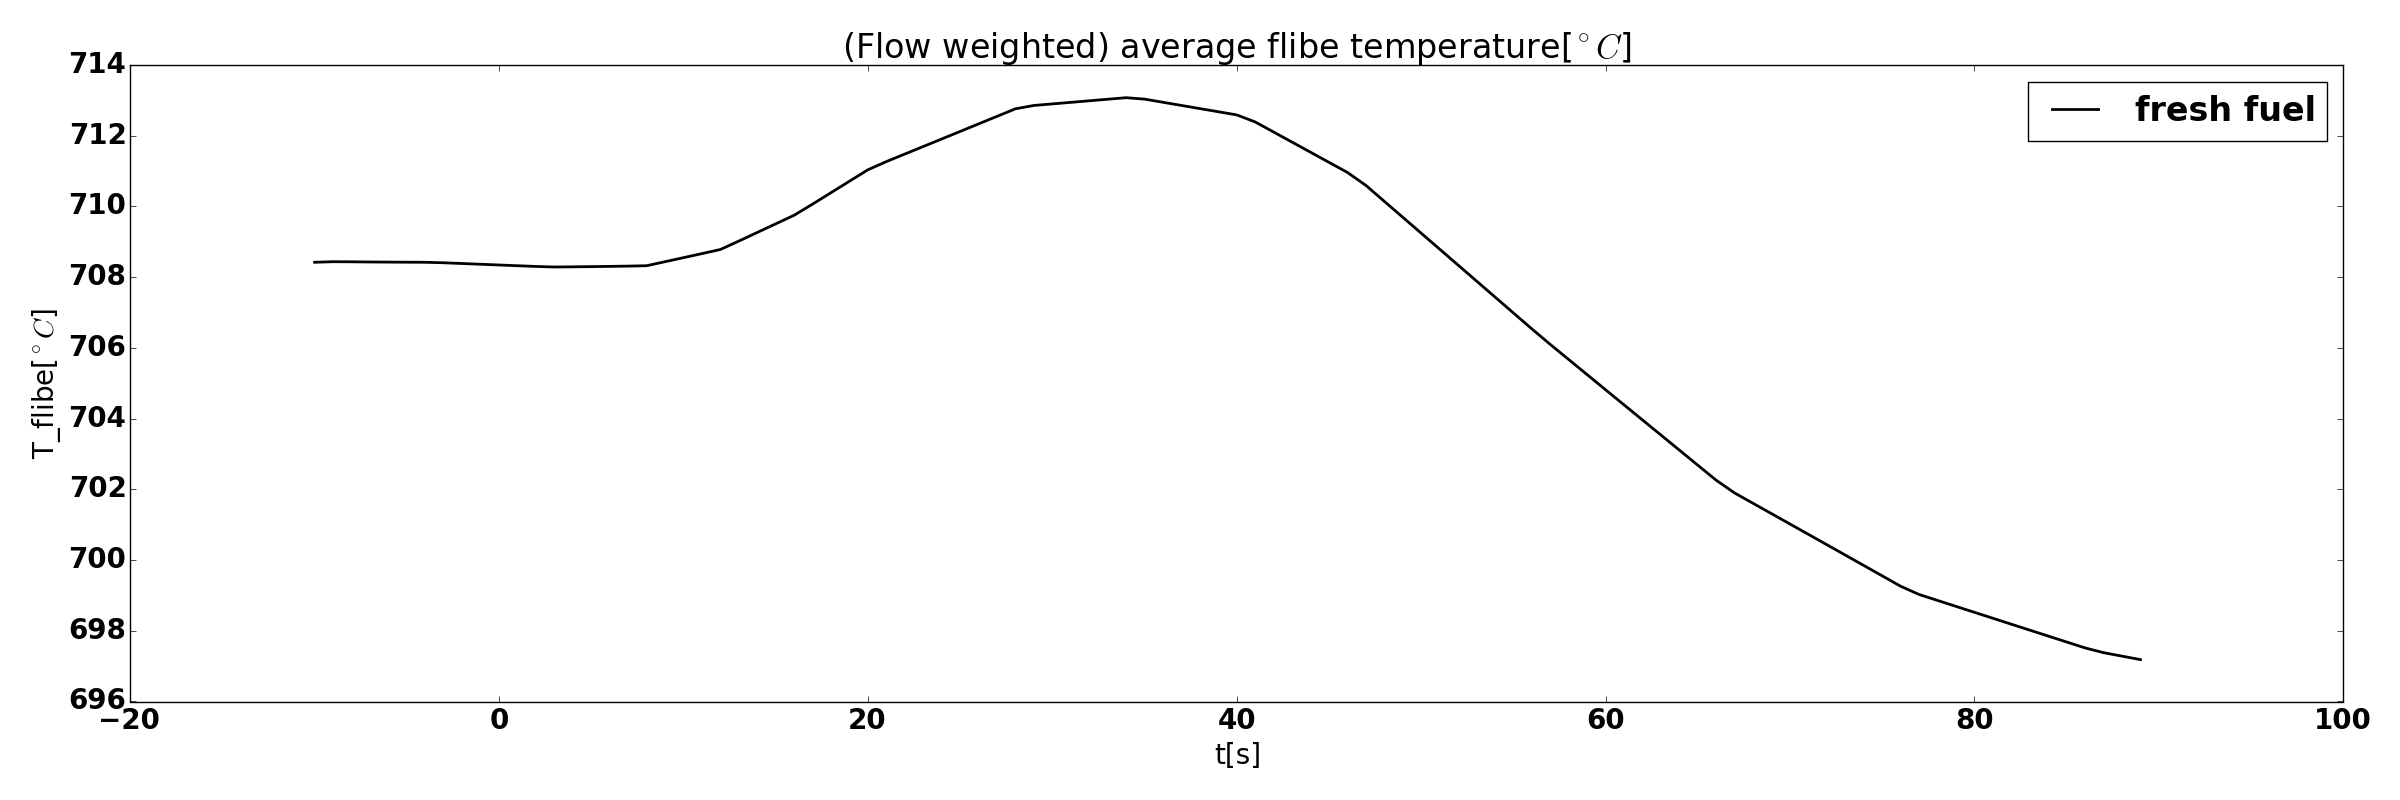
\includegraphics[width=\textwidth]{images/diffusion/mk1/OC/T_flibe_out.png}
    \caption{Average outlet coolant temperature during an overcooling transient}
    \label{fig:mk1_oc_t_out}
\end{figure}




\begin{figure}
    \centering
    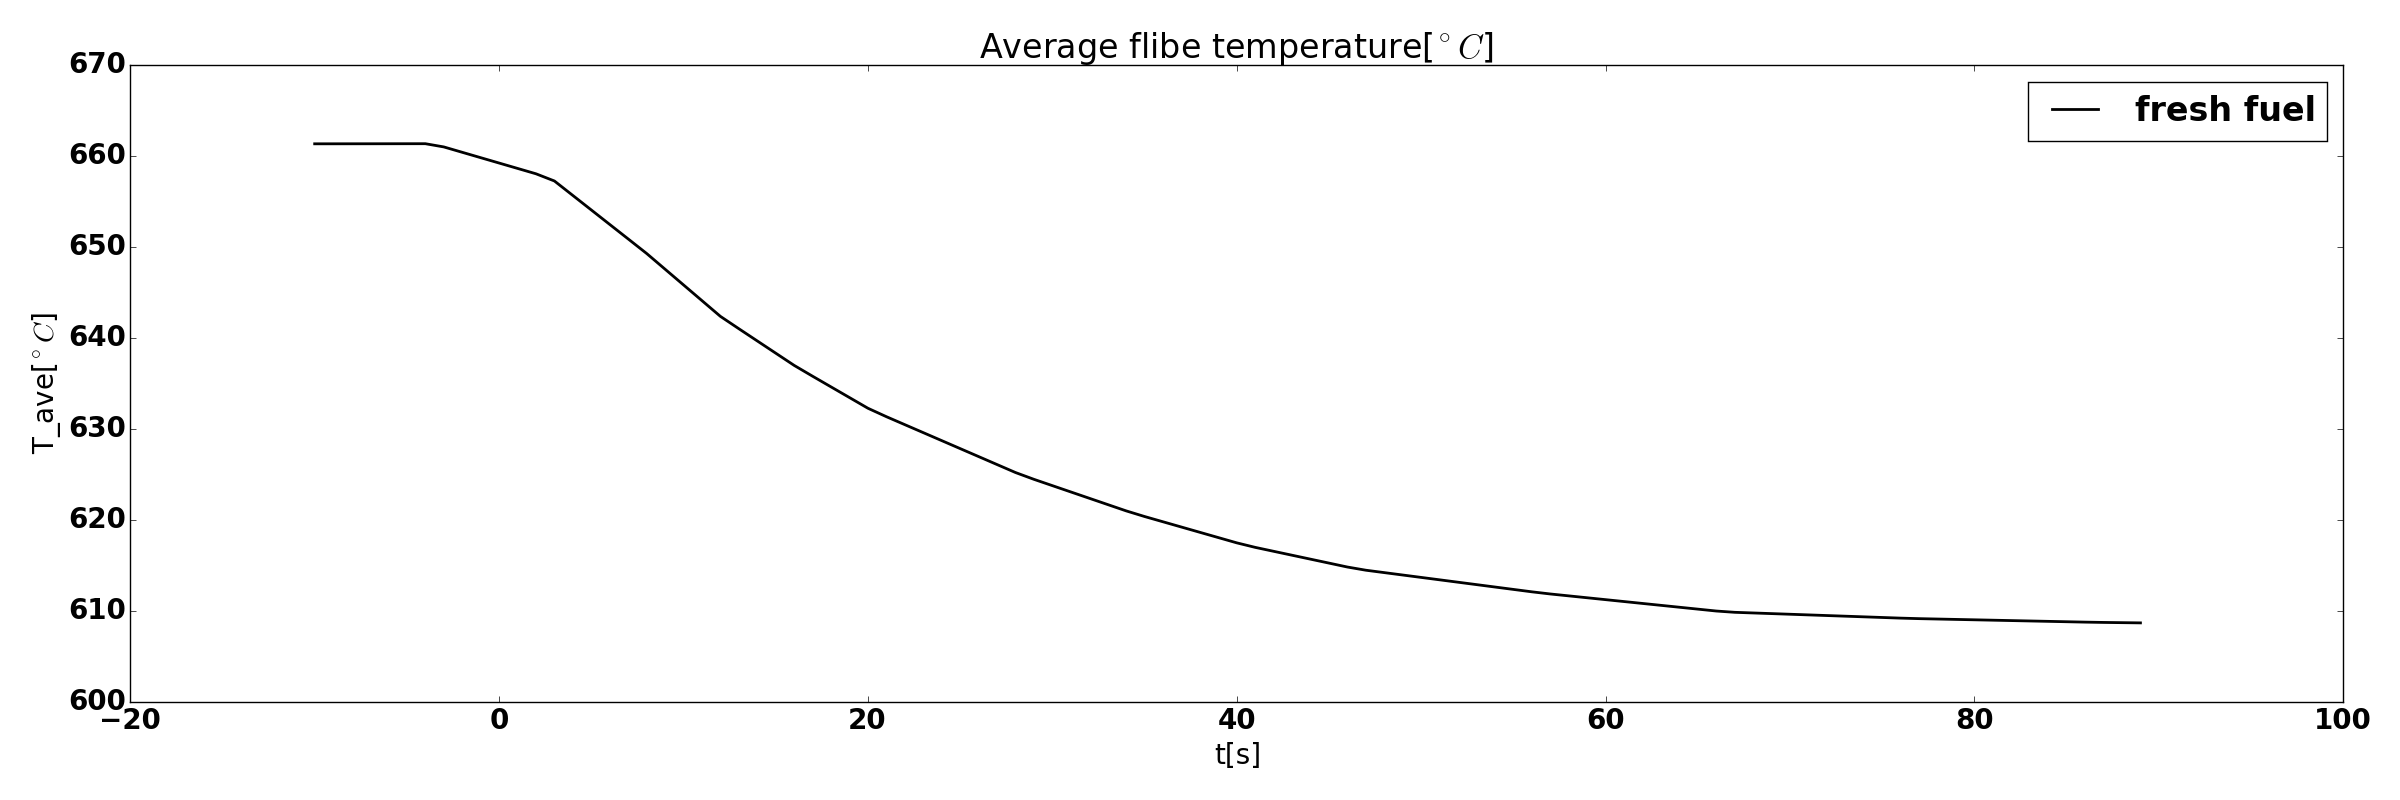
\includegraphics[width=\textwidth]{images/diffusion/mk1/OC/T_flibe_ave.png}
    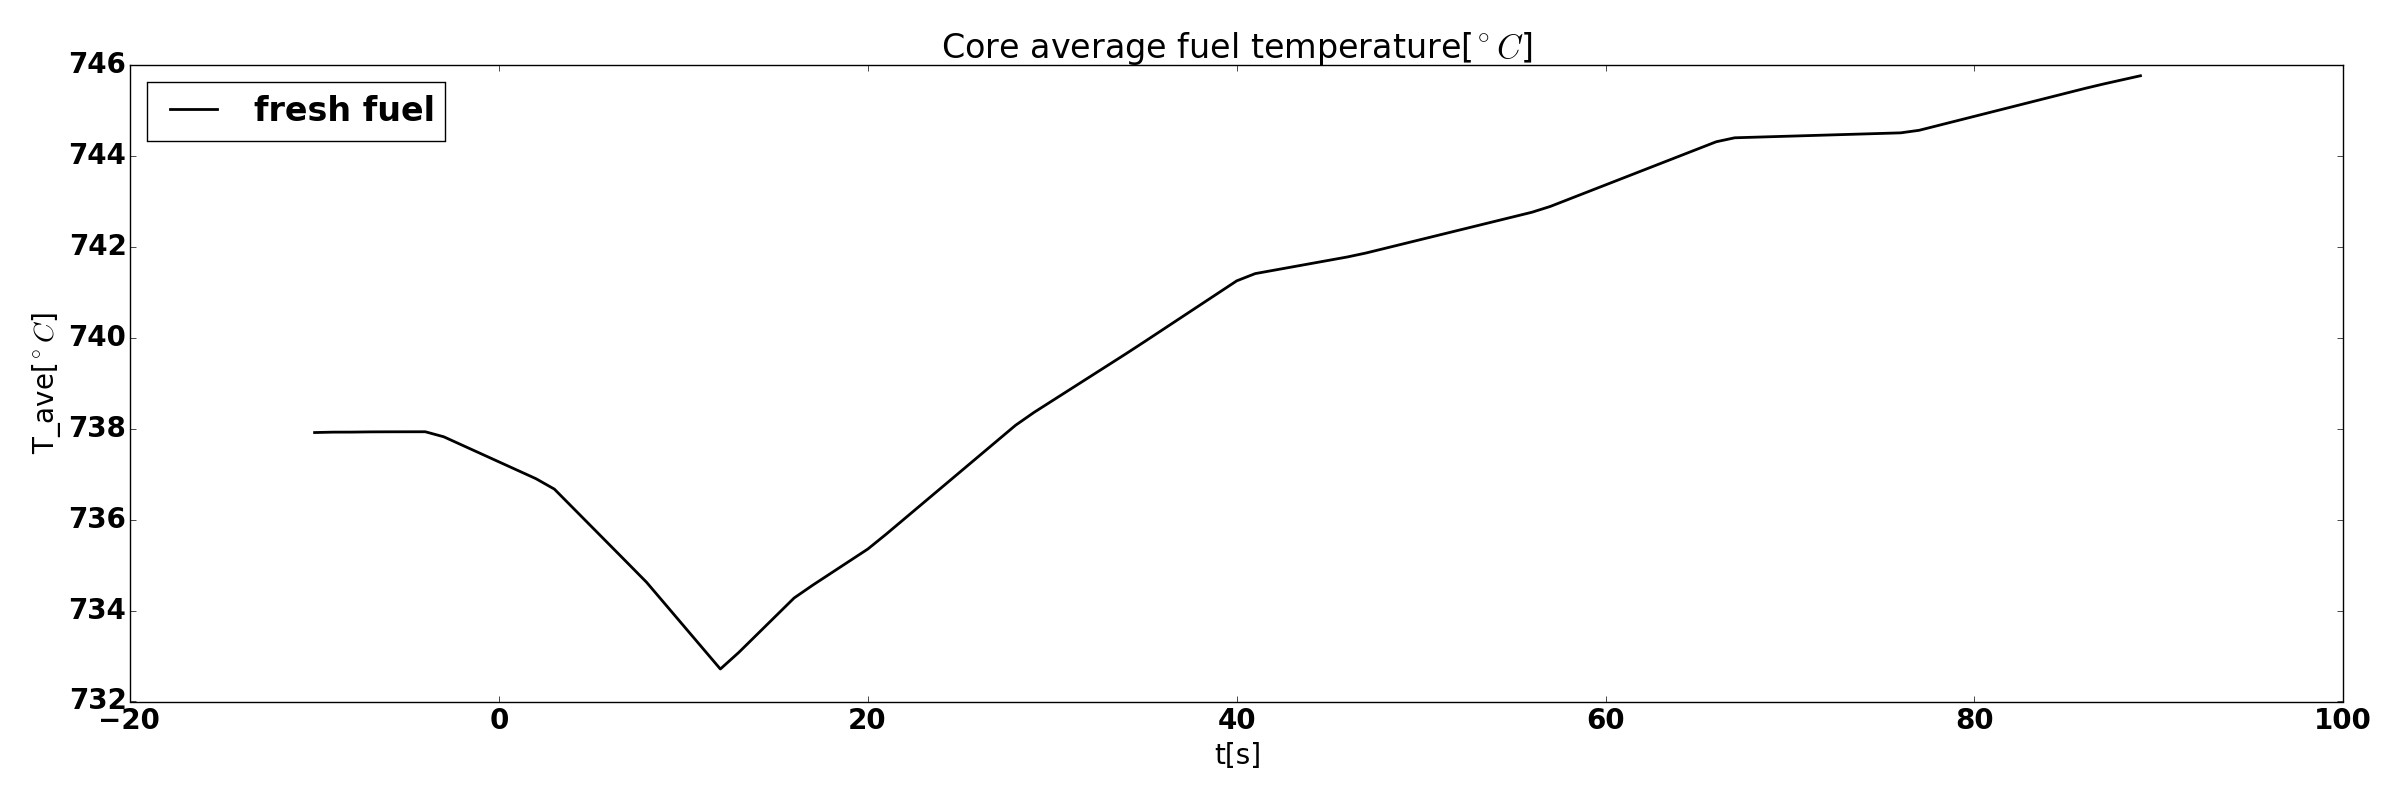
\includegraphics[width=\textwidth]{images/diffusion/mk1/OC/T_fuel_ave.png}
    \caption{Average fuel and coolant temperature during an overcooling transient}
    \label{fig:mk1_OC}
\end{figure}






In a ATWS transient, temperature feedback is the main mechanisms to stablize the reactor. The drop in core average flibe temprature is compansated by the increase in fuel temperature. Due to the larger Doppler feedback, the increase in fuel temperature is smaller than the decrease in coolant inlet temperature or in the average coolant temperature. 



\subsection{Control rod removal transients}
 Reactivity insertion (RI) can happen when one or more control rods, key elements in a reactor core for reactivity control, are extracted inadvertently. Control rod ejection caused RI is a common concern in LWRs, where the rapid removal of a control element from the pressurized system would cause an exponential increase in local and global power and temperature and may therefore cause critical damage to core integrity. However control rod ejection is not possible in FHR cores due to its low operating pressure. A control rod removal accident in a FHR would be more likely, although still very rare, to be caused by multiple failures of the reactor control system and thus the speed of the control rod removal would be limited by the designed maximum speed of the control rod  lifting system.


\begin{figure}
    \centering
    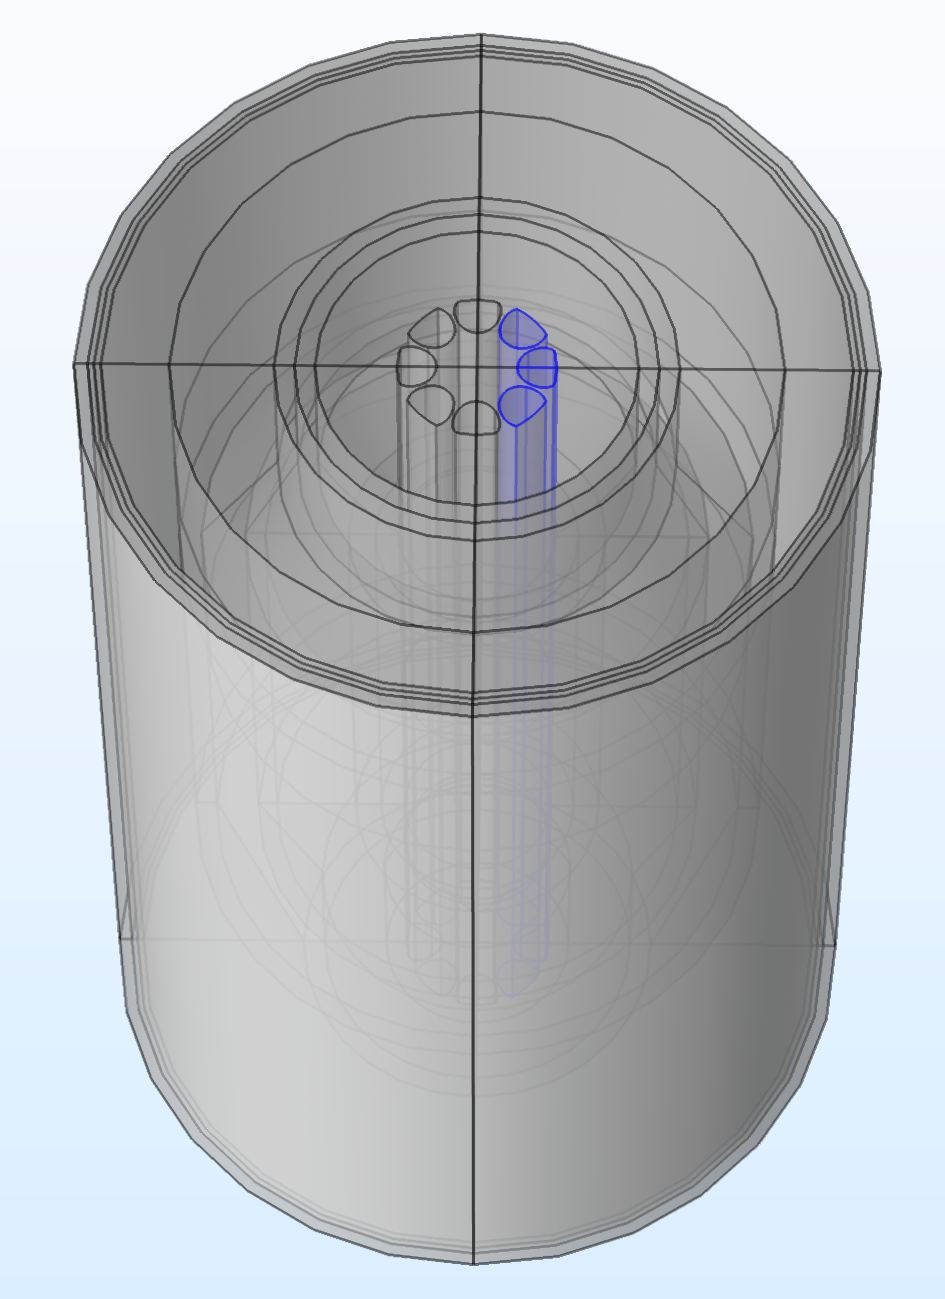
\includegraphics[width=0.3\textwidth]{diffusion/mk1/cr_RI/cr_removed.png}
    \caption{Illustration of removed control rods during the control rods removal transient}
    \label{fig:mk1_rods_removed}
\end{figure}




\begin{figure}
    \centering
    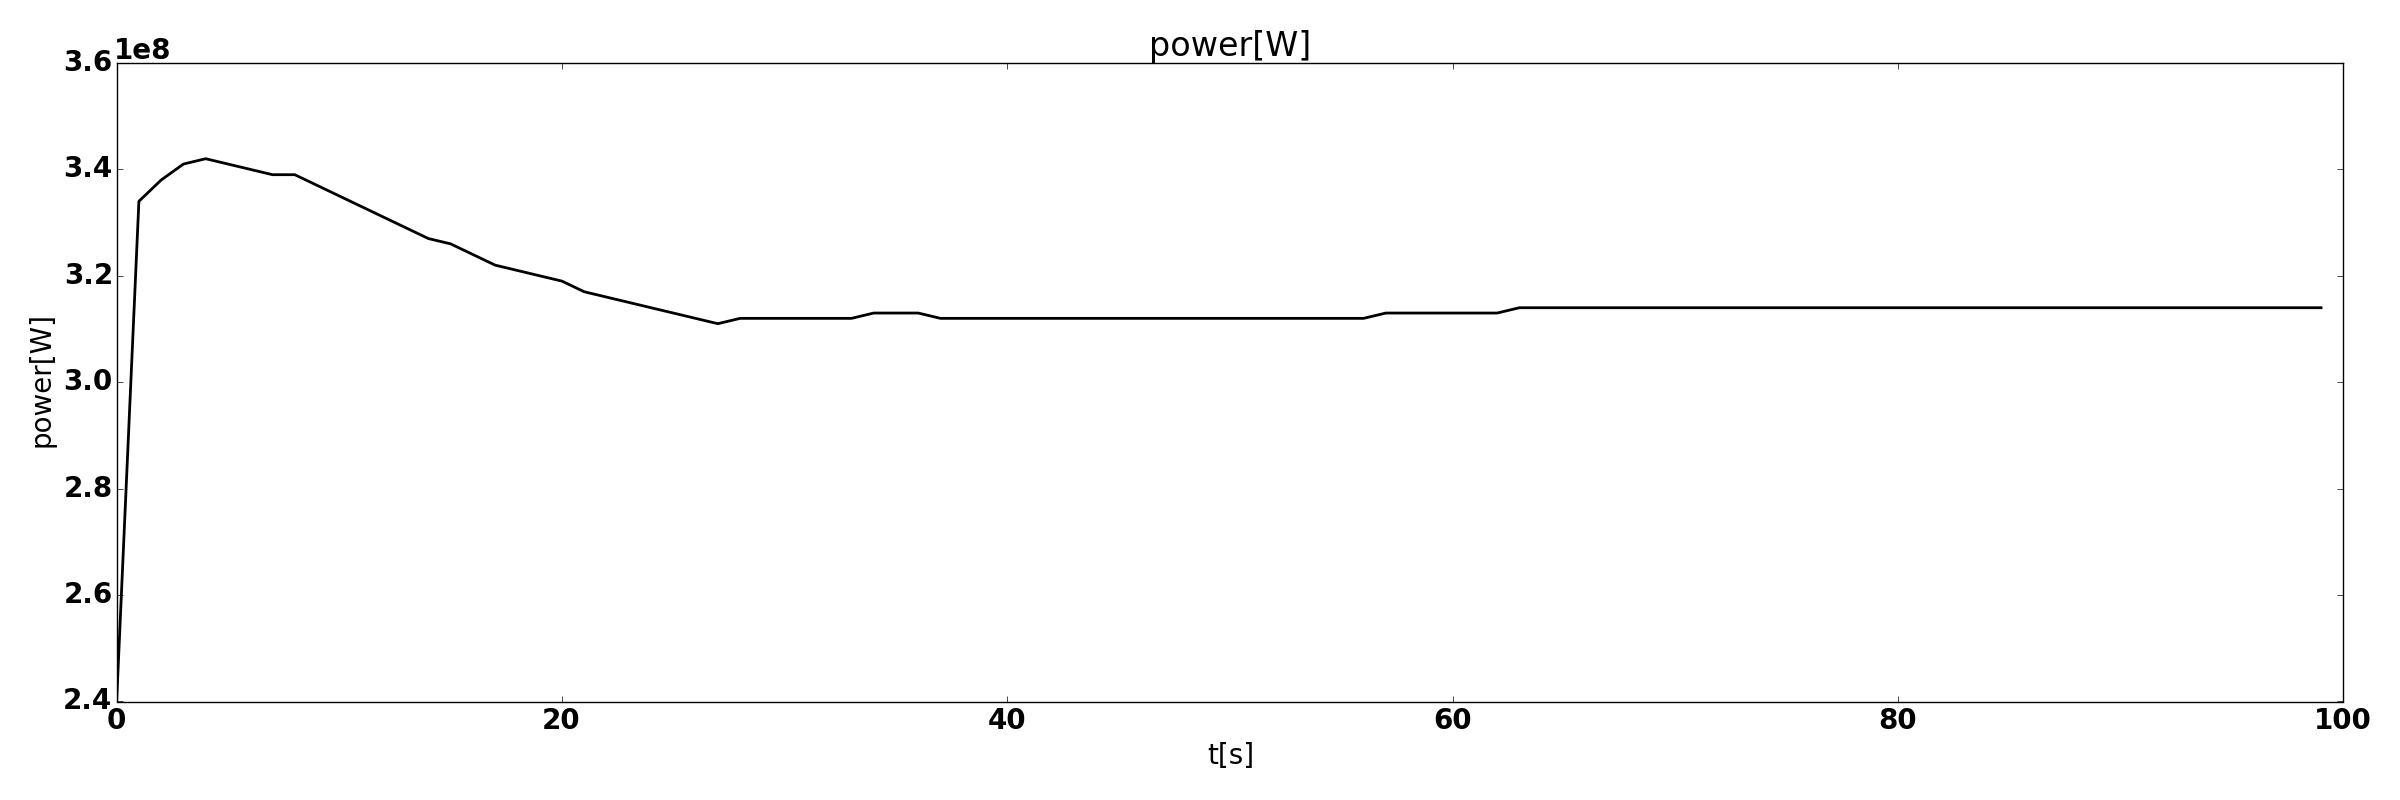
\includegraphics[width=\textwidth]{images/diffusion/mk1/cr_RI/power.png}
    \caption{Full core power during a control rod removal transient}
    \label{fig:multi_comp_power}
\end{figure}



\begin{figure}
    \centering
    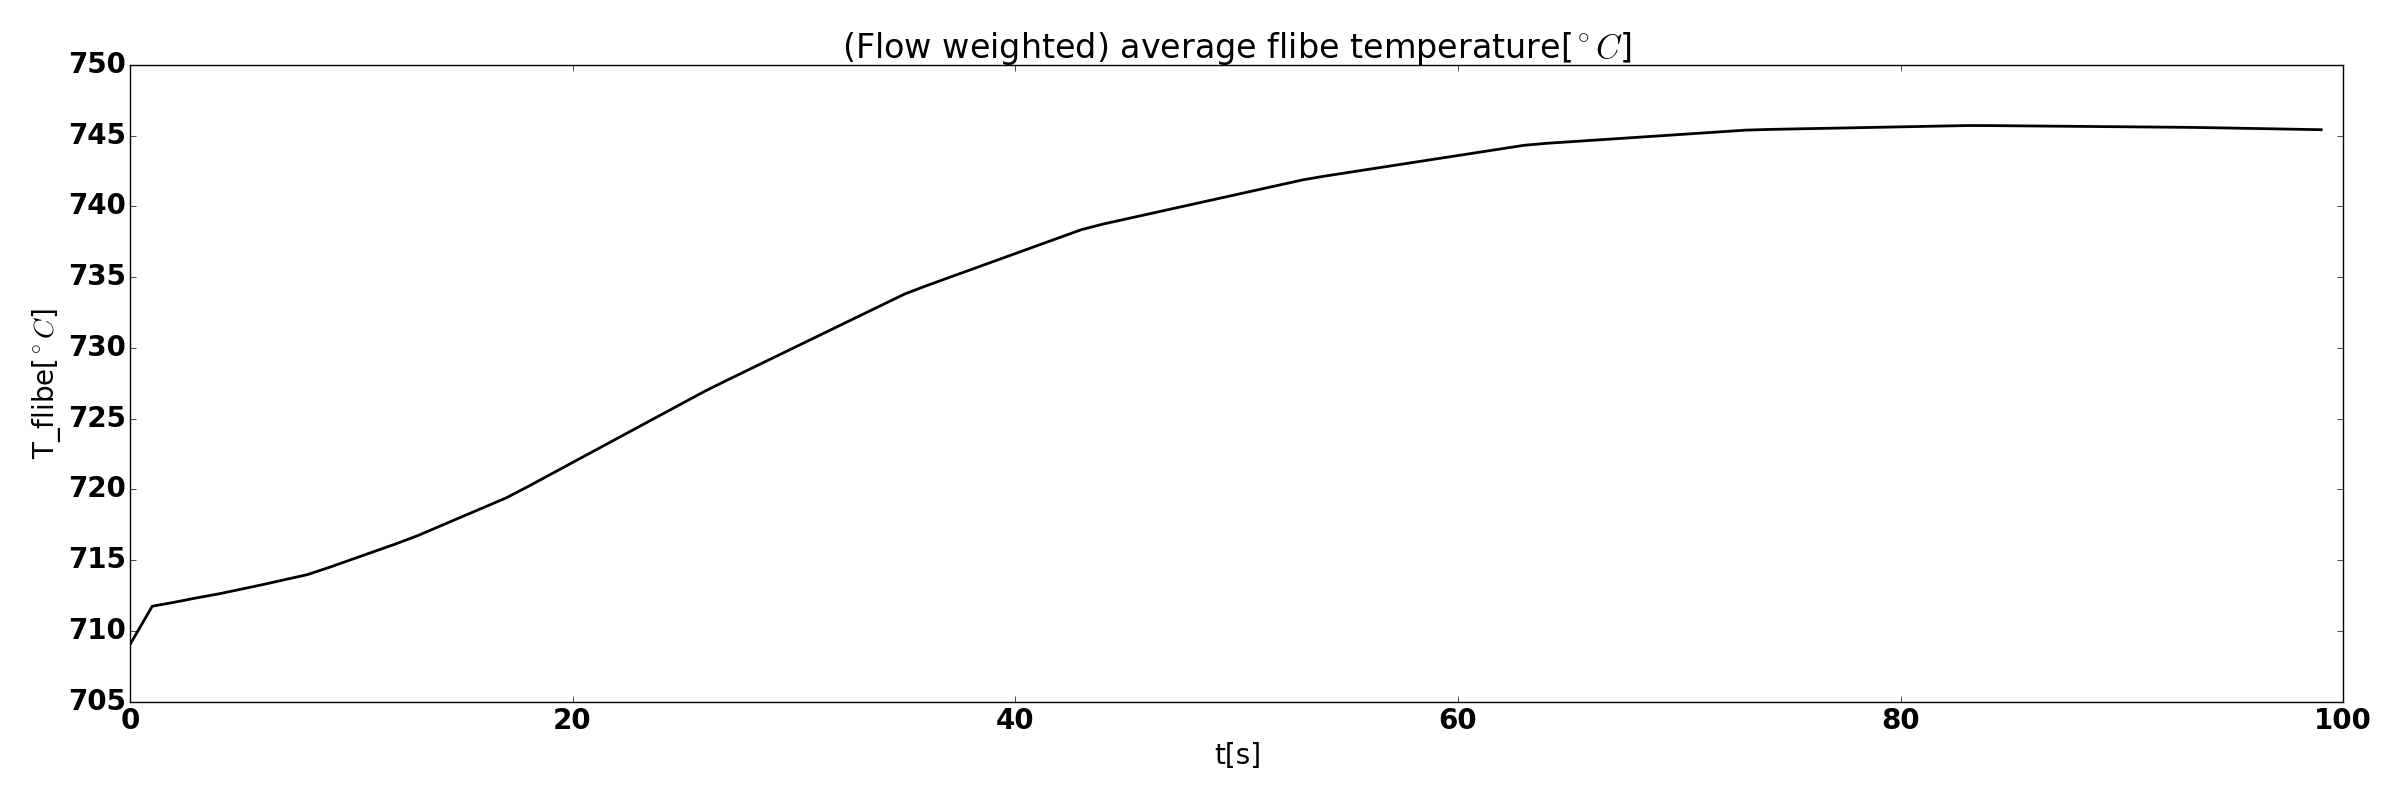
\includegraphics[width=\textwidth]{images/diffusion/mk1/cr_RI/T_flibe_out.png}
    \caption{Average output flibe temperatures during a control rod removal transient}
    \label{fig:cr_flibe}
\end{figure}

\begin{figure}
    \centering
    %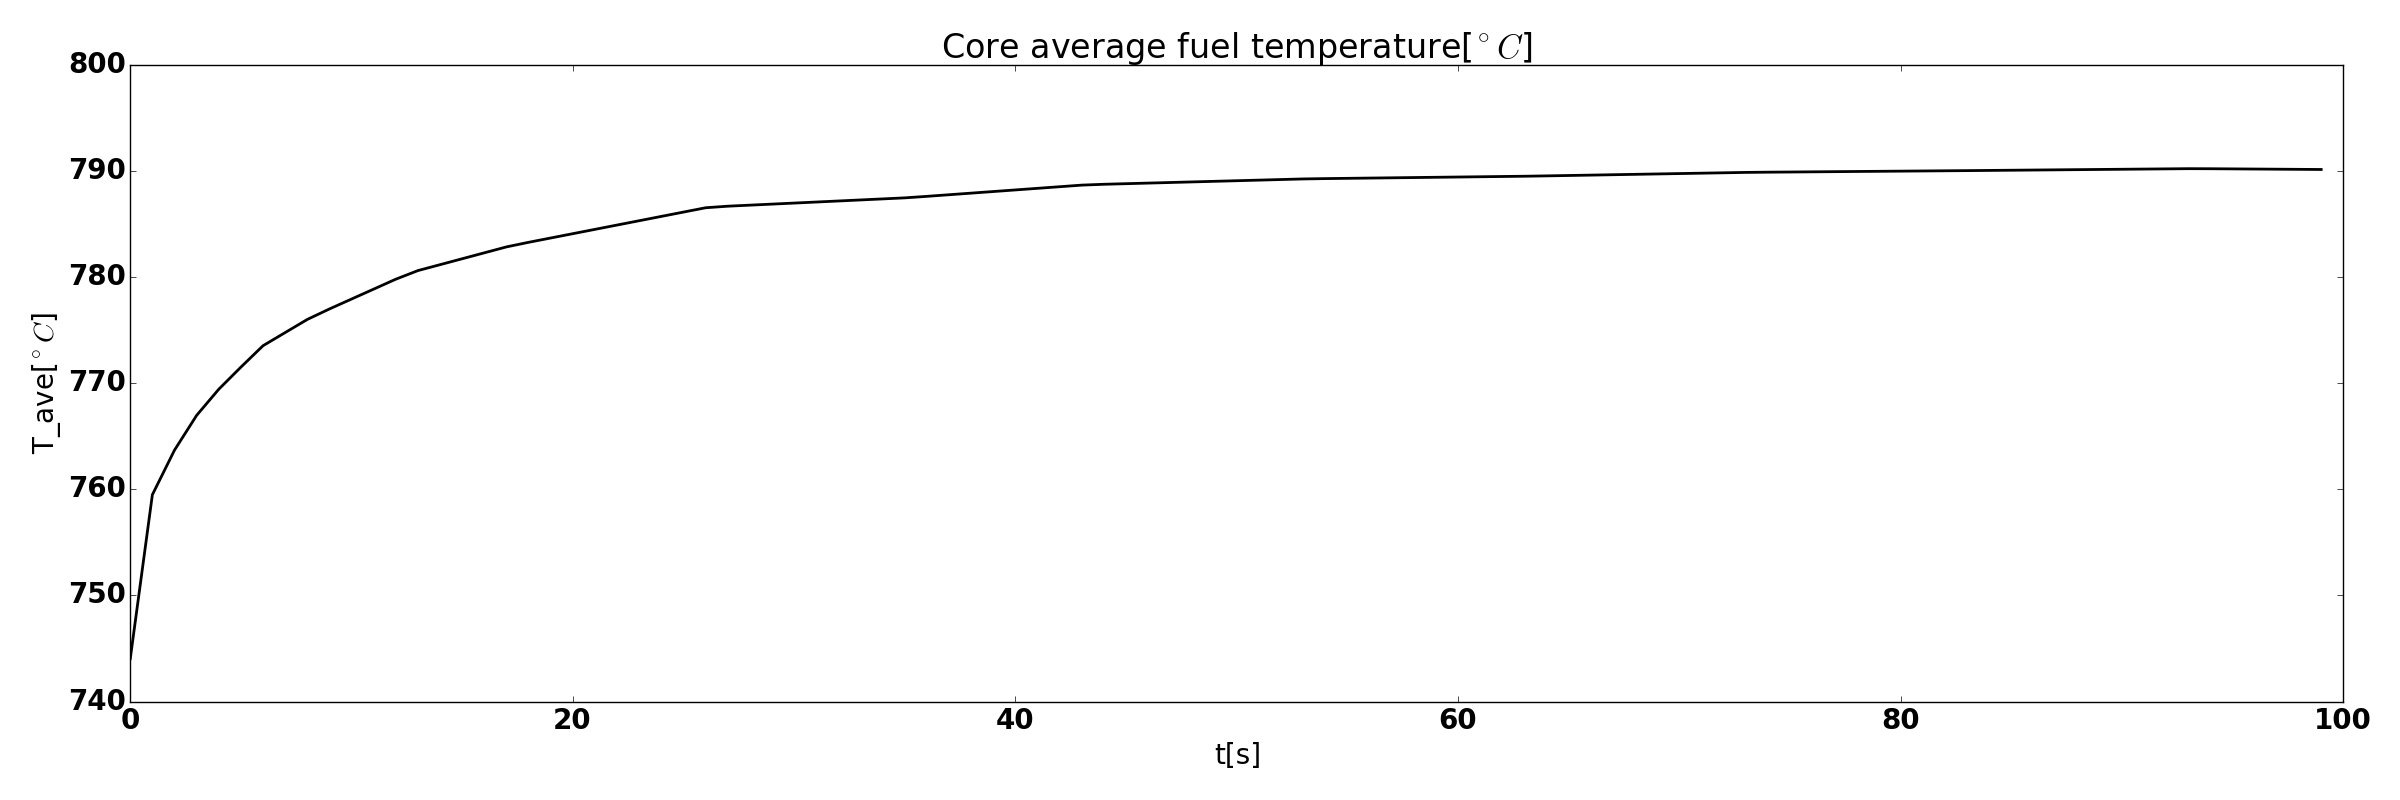
\includegraphics[width=\textwidth]{images/diffusion/mk1/cr_RI/T_fuel_ave.png}
    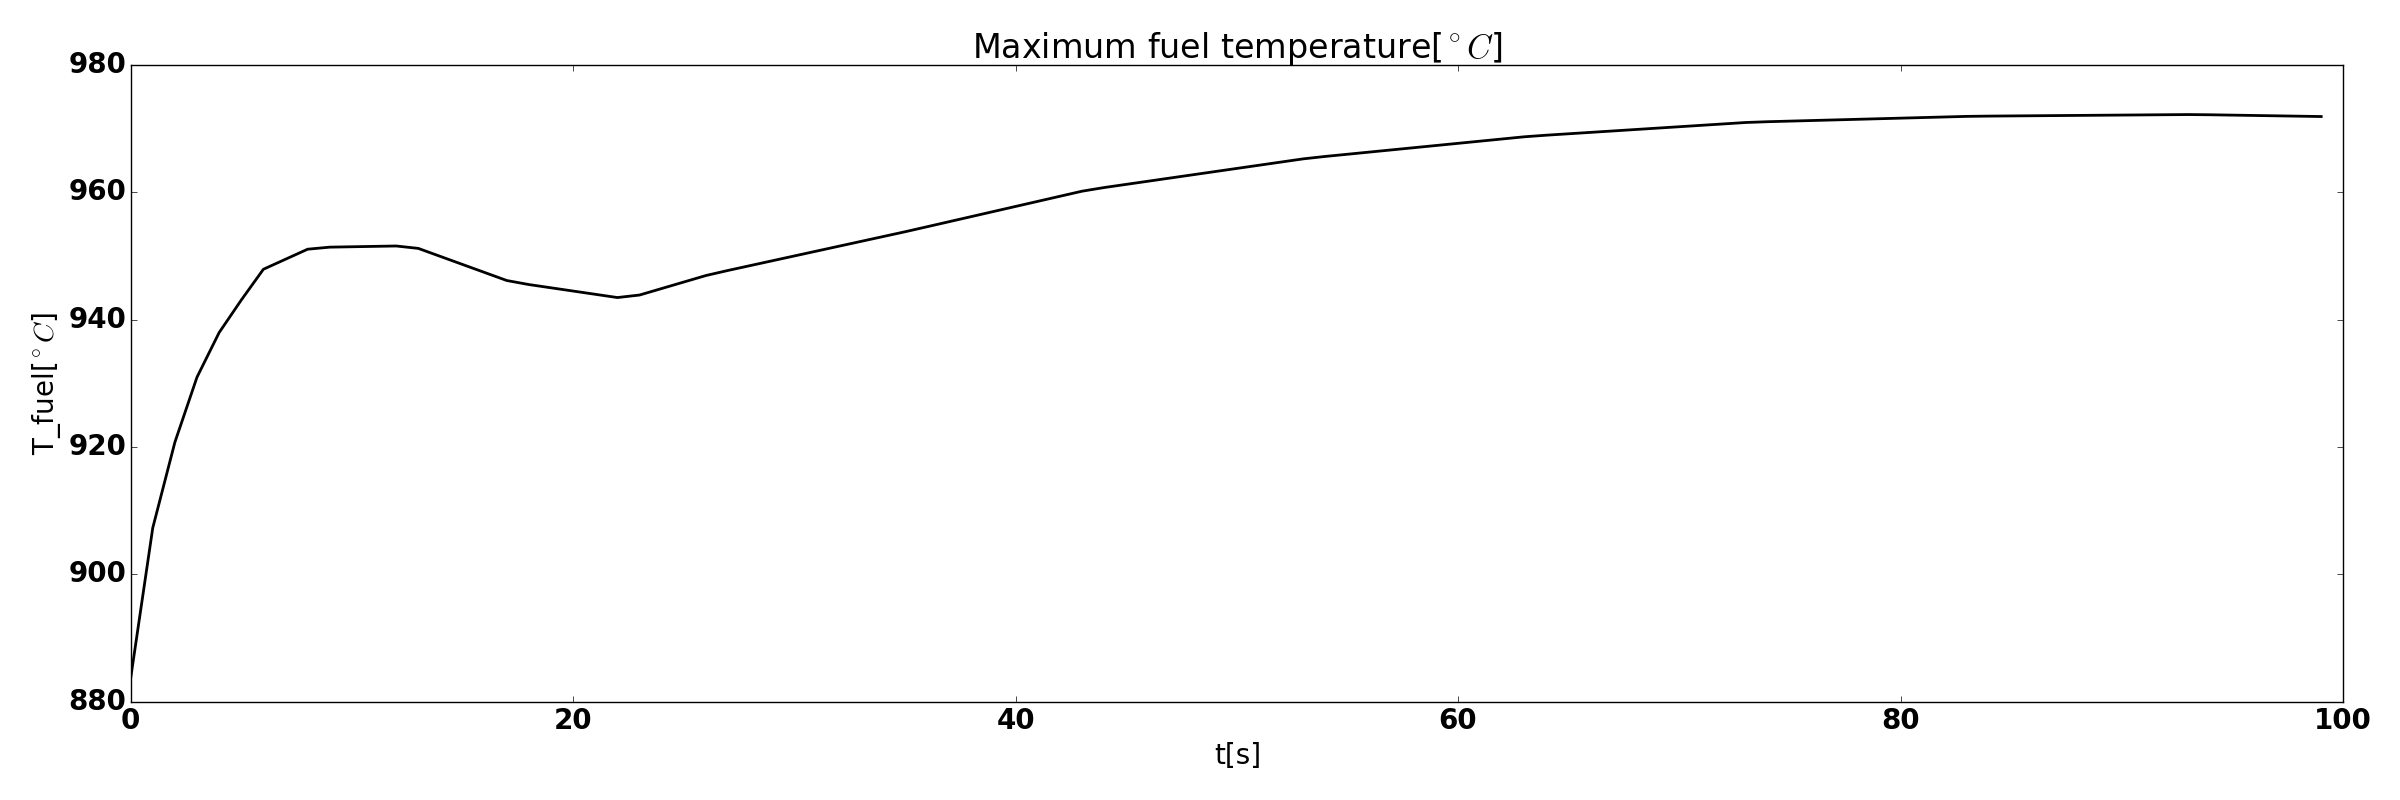
\includegraphics[width=\textwidth]{images/diffusion/mk1/cr_RI/T_fuel_max.png}
    \caption{Maximum fuel temperatures during a control rod removal transient}
    \label{fig:cr_fuel}
\end{figure}


Control rods are partially inserted to the core during normal operation for compensating excess reactivity, which is designed to ensure flexibility in operation. Reactors with online refueling design require a smaller excess of reactivity than those with batch refueling. Because of the continuous refueling, Mk1 can operate at very small excess reactivity, mainly for overcoming Xenon build-up during power sway.
To find the initial control rods position for the rod removal study, the control rods are inserted symmetrically to the height where the reactor would have 1.4\% excess reactivity \cite{Reitsma2012} if all rods are removed. 
And the transient is then triggered by removing three of the eight control rods from the core, illustrated in figure \ref{fig:mk1_rods_removed}. Because FHR cores are not under high pressure, so the speed of extraction would be limited by the control rods lifting machinery. While the detailed design for the lifting system is not yet available, prompt removal is simulated in this study to provide a bounding case for safety analysis. A parametric study on the effect of control rod lifting speed can provide guidance on how fast should we design the control rod lifting system. 


Figure \ref{fig:multi_comp_power} shows the full core power during the transient. The power increases at first due to the inserted reactivity and stabilize at a slightly higher level due to temperature feedback from the fuel elements and the coolant. The peak power during this transient is about 50\% above the initial power. 
Figure \ref{fig:cr_flibe} shows the average coolant outlet temperature weighted by the flow. This parameter reflects the coolant temperature when it arrives at the hot leg pipes after efficient mixing. 
The flow weighted average coolant outlet temperature represents the coolant temperature at the hotleg after mixing in the upper plenum. It is increased by about 30 \degc\  and remains below 750 \degc\ during this simulated transient.
Figure \ref{fig:cr_fuel} shows the maximum fuel temperature, i.e. the temperature of the center of the fuel kernel at the hottest location in the core. It is far below the safety limit during this transient.


% \subsection{External reactivity insertion}
% Although unlikely, a large external reactivity insertion to the core is a good study case for code verification, because it challenges the code's ability to capture rapid changes in the core. 


% 1\$ external reactivity is inserted into a Mk1 core with equilibrium fuel at nominal operating condition.



% Analyze the variation in different burnups... Fresh VS old pebbles




\subsection{Seismic reactivity transients in Mk1 core}
A special class of reactivity related transients for pebble-bed FHRs is the pebble densification during an earthquake. 
The safe shutdown earthquake event has been identified as a Design Basis Accident (DBA) in the licensing basis event selection for the Pebble Bed Modular Reactor (PBMR) and in the Chinese HTR-10 certification \cite{Reitsma2012}. 
To meet licensing requirements and to optimize the design under DBAs, this type of transient is investigated for Mk1 pebble bed reactor design.

The seismic wave causes movement of the fuel pebbles, increases the packing fraction of fuel pebbles and cause transients in the core. 
The density of the Mk1 fuel pebbles are adjusted so that the pebbles are buoyant in the coolant. So unlike helium cooled pebble bed reactors, the pebbles in a Mk1 core would rise towards the top of the core during an earthquake due to the motion caused by the shaking of the vessel. This results in fuel densification toward the top and leaves the bottom of the core with only coolant.
The Mk1 control rods are inserted from the top, therefore, they remain effective and may actually provide negative reactivity during this transient.

While the exact magnitude of the compression and the timescale depends on the earthquake and needs to be determined by discrete element modeling and shake table studies, we can investigate the effect of pebble compression on core neutronics by comparing the core reactivity before and after a postulated increase in packing fraction. The impact of changes in the coolant passage geometry on coolant flow is not considered in this study.
We have compared the multiplication factor of the core under different pebble packing fraction, between the nominal operating packing fraction 60\% and the maximum attainable pebble packing fraction due to earthquake induced shaking - 64\% (\cite{Radin2008}\cite{Chen2018}). The change in \keff with respect to the nominal packing fraction (60\%) is listed in table \ref{tab:pk_earthquake}. 

\begin{table}[h]
    \centering
    \begin{tabular}{lcc}
      Packing fraction   & $\Delta$\keff* [pcm] & uncertainty** [pcm]\\
        61\% & - 24 & 1.2\\
        62\% & - 52 & 1.2\\
        64\% & - 236 & 1.2\\
    \end{tabular}
    \caption{Change in \keff during an earthquake with different amount of fuel densification (* $\Delta$ \keff = \keff$_{denser}$ - \keff$_{60\%}$,  **uncertainty: uncertainty associated to Monte Carlo computation)}
    \label{tab:pk_earthquake}
\end{table}

The results show that the core reactivity decreased by a small amount after the increase in packing fraction.
In fact, the Mk1 core is optimized to have negative coolant void feedback at nominal conditions with equilibrium fuel composition. Thus if a postulated earthquake occurs at nominal condition, the reactivity would decrease due to 'loss' of coolant in the fuel pebble region.
Flibe salt has stronger neutronic properties than helium due to its higher density. This can be a safety advantage in some transient scenarios. 
However, it is worth noting that the resulting reactivity change in a Mk1 core during an earthquake depend on the initiation point. Fuel composition, temperature, power level, Xenon concentration, etc. all play a role in determining the coolant reactivity feedback coefficient, which is one of the main parameters that drives the reactivity change. In order to ensure the safety design of a Mk1 core, one would need a comprehensive study of all possible scenarios and optimize the design with respect to the bounding case.




% \newpage
% \section{Uncertainty quantification and sensitivity analysis}
% \label{sec:uqsa_mk1}

% When building numerical models, we often face the question of which value we should use for some input parameters. Inputs for FHR models are uncertain due to lack of knowledge or intrinsic variations, including difficulties in measuring thermophysical properties and nuclear data, flexibility in design, material changes during operation due to radiation, fatigue, and ambient temperature, geometry change due to thermal expansion and radiation induced swelling, and etc. 
% Correlations are often used in thermal-hydraulics modeling, and they introduces uncertainties from approximating a complex flow phenomena by a empirical relationship of characteristic dimensionless numbers. 

% Uncertainty quantification and sensitivity analysis(UQSA) needs emerge when the inputs of a numerical model are not known with certainty.
% Uncertainty analysis characterizes the spread of the response function and sensitivity studies compute the contribution of an individual parameter on the uncertainty. 


% An UQSA study workflow consists of the following steps:
% \begin{itemize}
%     \item{Identify all the uncertain input parameters and output variables.}
%     \item{Screening or feature selection to reduce the number of variables that are considered in an UQSA study.}
    
%     \item{Sampling input variables and generating database of model outputs}
    
%     \item{Analyze uncertainty from estimated statistical summary of output distribution, such as mean, variance, a certain percentile.}
% \end{itemize}

% This chapter starts by identifying sources of uncertainty in an FHR model. Also selected in section \ref{sec:uncert_param} are the output variables, based on their importance to reactor safety. The uncertainty is propagated through the model in section \ref{sec:UQSA}.


















% \section{Source of uncertainty}
% \label{sec:uncert_param}
% The first step of a UQSA study is to identify the source of uncertainties in the input parameters and to select key output variables(also called figure of merit), of which the uncertainty is studied.
% % Independent or isolated groups

% In a multiphysics model for FHRs, the uncertainty stems from the following aspects:



% \begin{itemize}
%     \item{Material properties}
%         \begin{itemize}
%             \item mod\_k, fuel\_k and shell\_k: thermal conductivity for moderator, fuel and shell[w/k.m]
%             \item mod\_cp, fuel\_cp, shell\_cp and cool\_cp: specific heat capacity of moderator, fuel, shell, and coolant[J/kg.k]
%         \end{itemize}
%     \item{Nuclear data}
%             \begin{itemize}
%                  \item  cool\_feedback: temperature reactivity feedback coefficient of the coolant[pcm/k]
%                   \item Doppler: Doppler temperature reactivity feedback coefficient of the fuel[pcm/k]
%         \end{itemize}
%     \item{Geometry}
%         \begin{itemize}
%             \item{TRISO particle diameter, variation in packing fraction, }
%         \end{itemize}
    
%     \item{Empirical correlations}
%     \begin{itemize}
%           \item h: convective heat transfer coefficient[w/m2.k]
%           \item{Pressure drop[Pa]}
%     \end{itemize}
%     ...

% \end{itemize}

% The uncertainty in each input parameter is expressed by a probability distribution, estimated by expert judgment, manufacturer of the nuclear reactor components, experiments and previous calculations.







% % Independent parameter can be determined by perturbation.
% % Correlated ones need to be considered together. Sampling methods to efficiently cover the high dimensional space. 







% \section{UQSA methodology}
% \label{sec:UQSA}


% A computer model computes an output y from input x, noting $y=f(x)$. The input parameters for computer code are often known with uncertainties, so users of such models often wish to consider the output variation when one or more input parameters are uncertain.
% UQSA uses statistical methods to determine likely effect of variation in model inputs on the simulation outcome.


% \subsection{Uncertainty quantification}

%  Uncertainty study considers the input parameter or vector of parameters as a random variable with probability distribution G(X), and consequently compute the distribution of the output $Y=f(X)$. Uncertainty regarding inputs is characterized by a (joint) probability distribution for their values. This distribution induces a (joint) probability distribution for the output, and uncertainty analysis involves identifying that distribution. 

% Summary statistics, such as the mean and the variance of the output uncertainty distribution are often computed, as in equation \ref{eq:mean_and_var}. The mean can be a best estimate for the output value, while the variance measures its spread due to input uncertainty. In some applications, it is also important to calculate the confidence intervals. 
% NRC uses an 95-95 tolerance limits in safety system setpoint analysis, which is a confidence interval that bounds 95\% of population with 95\% likelihood\cite{Rahn2010}. This corresponds to an interval width of $\pm1.96\sigma$ if the value follows a normal distribution.




% \begin{align}
%   \label{eq:mean_and_var}
%   E[f(x)] = \int_x f(x) w(x) dx\\\nonumber
%   Var[f(x)] = \int_x (f(x) - E[f(x)])^2 w(x) dx
% \end{align}




% \subsection{Sensitivity analysis}
% Sensitivity study investigates how the variation in the output of a model can be apportioned to different source of uncertainty.
% (Variance-based) sensitivity analysis considers the variance of the output, described as a joint probability distribution.
% If we were to remove the uncertainty in the ith input $X_i$, we would expect the variance of the function output f(X) to decrease. We can compute the variance of the conditional expectation(VCE) of prediction $Var[E(f(X)|x)]$ and the correlation ratio, defined in equation \ref{eq:eta}, as the contribution in the output variance by the ith input uncertainty, a.k.a. its sensitivity.

% \begin{equation}
% \eta ^2 = \frac{Var[E(f(X)|x]}{Var[f(X)]}
% \label{eq:eta}
% \end{equation}

% Sensitivity study methods can be sorted into two general categories: local sensitivity study and global sensitivity study. Local sensitivity study aims to compute the change in the output due to minuscule amounts of changes in the input. Local sensitivity study computes the partial derivatives of the output with respect to the inputs, evaluated at the base values. Global sensitivity study analyzes larger amount of changes, and therefore can not rely on local derivatives but instead needs to generate the probability distribution over the entire space. 







% \subsection{UQSA methods}
% \label{sec:sampling}

% The Monte Carlo method is the most widely used and easiest method to setup for compute the summary statistics discussed in the previous sections, where random samples are drawn from the input probability space and the model is run repeatedly at each input set. Latin-hypercube sampling method covers the multi-dimensional space more efficiently by stratifying each of the d components and sample randomly within each strata. 

% An illustration of a Latin-hypercube(also called a Latin square in 2-D) is shown in figure \ref{fig:LHS}.

% \begin{figure}[h]
%   \centering
%   \includegraphics[width=0.6\textwidth]{./images/latinHypercube.png}
%   \caption{Illustration of a Latin-hypercube}
%   \label{fig:LHS}
% \end{figure}





% \subsection{Bayesian inference for functions}
% \label{sec:bayesian}
% There are two major schools of thought about probability: Bayesian and Frequentist. Frequentists views probability as an asymptotic proportion of an event in an infinite number of trials.
% While the Bayesian reasoning thinks of probability as a degree-of-belief. It is preferred because it allowing us to treat unknown output variables as random variables even if the computer code is deterministic, in the sense that we are not sure what the values would be until we run the code.
% The basis of Bayesian inference lies on the fundamental relationship of conditional probabilities: the Bayes' theorem (\ref{eq:Bayes}).
% Bayesian inference starts by posing a probability distribution for the unknowns(prior distributions p(A)), which reflects the current state of knowledge about their possible values. These prior distributions are then updated as new information are available, resulting in the posterior probability distribution: the conditional probability of event A given B(p(A|B)).
% \begin{equation}
%   p(A|B) = \frac{p(B|A)p(A)}{p(B)}
%          = \frac{p(B|A)p(A)}{\int p(B|A)p(A) dA}
%   \label{eq:Bayes}
% \end{equation}


% Under Bayesian formulation, we treat the output of deterministic computer code as random variables, in the sense that it is an unknown quantity until the model is run.
% We pose a prior distribution on the random function as our prior belief of how the function responds to input parameters and compute its posterior distribution after observing the data.

% In practice, the observed outputs $(y_1, y_2, \dots y_n)$ may not be the exact function value but the real value with noise ($f(x) + \epsilon$) for many modeling situations, e.g. Monte Carlo based simulations. The inference problem is to estimate $f(x_*)$ for other values of x, note $x_*$, using the observed data. The following sections discuss inference about functions using Gaussian processes prior and noisy data.






% \subsubsection{Gaussian processes}
% \label{gp}

% Gaussian processes with specified mean and variance function are typically used to model computer simulations in various field\cite{Haylock1996}\cite{Bhattacharya2007}\cite{Yurko2014}. This project investigates Gaussian processes and formulates a methodology for developing a Gaussian processes emulator for nuclear reactor simulation codes. 

% The Gaussian process is the extension of the multivariate normal distribution to infinite numbers of dimensions. A Gaussian process model $f(.)$ can be defined solely by its mean function $m(.)$ and covariance function $k(.,.)$.
% \begin{eqnarray}
%   f(.) \sim GP(m(.), k(.,.))
%   \label{GPprior}
% \end{eqnarray}

% This means that each individual $f(x)$ is normally distributed as:
% \begin{eqnarray}
%   f(x) \sim N(m(x), k(x,x))
% \end{eqnarray}

% and the joint distribution of the values of $f(x)$ at any finite number of different x values is multivariate normal. We rely on the assumption of smoothness of the function such that there is a higher correlation between $f(x)$ and $f'(x)$ when x and x' are closer.
% \begin{eqnarray}
%   Cov(f(x), f(x')) = k(x, x')
% \end{eqnarray}

% Assuming that the noise are independent from each other and that they each follow the Gaussian distribution $\epsilon \sim N(0, \sigma_n^2)$, the prior distribution of y is:
% \begin{eqnarray}
%   y \sim GP(m(.), k(.,.) + \sigma_n^2 I)
%   \label{yprior}
% \end{eqnarray}

% Prior information about how $f(.)$ responds to input x may come from knowledge of the real life phenomena that the code is simulating. In general, we state that
% \begin{eqnarray}
%   m(x) = h(x)^T \beta\\
%   k(x,x') = \sigma_f ^2 c(x, x'),
% \end{eqnarray}


% and the prior model for $f(.)$ conditioned on the parameters is given by
% \begin{eqnarray}
% f(.) | \beta, \sigma_f ^2 \sim N\{h(.) ^T\beta, \sigma_f^2c(.,.)\}.
% \end{eqnarray}

% h(x) are a set of fixed basis functions that can incorporate expert knowledge about the underlying physics.
% $\beta$ is unknown parameter that can be determined by maximum likelihood optimisation along with other parameters or often modeled with a gaussian prior:
% \begin{eqnarray}
% \beta \sim N(\bar{\beta}_0, \Sigma_{\beta0})
% \end{eqnarray}

% Integrating over the prior distribution of $\beta$, the distribution of f is a Gaussian process
% \begin{eqnarray}
%   f(x) \sim GP(h(x)^T\bar{\beta_0}, k(x, x')+h(x)^T\Sigma_{\beta0}h(x')
% \end{eqnarray}

% A widely used correlation function\cite{Seeger2004a} is the squared exponential covariance function:

% \begin{eqnarray}
%   c(x, x') = exp\{-\frac{1}{2}(x-x')^TB(x-x')\}
% \end{eqnarray}

% equivalently, the covariance matrix for y is:

% \begin{eqnarray}
%   k_y(x_p, x_q) = \sigma_f^2exp\big[\frac{-(x_p-x_q)^TB(x_p-x_q)}{2}\big] + \sigma_n^2I
% \end{eqnarray}

% where B is a diagonal matrix of smoothing parameters that can be choosen by cross validation or expert knowledge. The higher an element in B is, the smoother $f(.)$ is and the higher the coorelation between two points $f(x)$ and $f(x')$ will be.






% \subsubsection{Posterior inference}
% The joint distribution of the observed response variables y and the function values at the test locations $X_*$ under the prior is

% \begin{eqnarray}
%   \left[ \begin{smallmatrix} y\\ f_* \end{smallmatrix} \right] 
%   \sim 
%   N(\left[ \begin{smallmatrix} m(x)\\ m(x_*) \end{smallmatrix} \right], 
%       \left[ \begin{smallmatrix} K(X, X) + \sigma_n^2I & K(X, X_*)\\ 
%         K(X_*, X) & K(X_*, X_*) \end{smallmatrix} \right]) 
% \end{eqnarray}

% The posterior distribution of $f_*$ given the observed data is another Gaussian process

% \begin{eqnarray}
%     f_*|X, y, X_* \sim N(\bar{f_*}, cov(f_*)\\
%     \bar{f_*} = H_*^T\bar{\beta}+ K(X_*, X)K_y^{-1}(y-H^T\bar{\beta})\\
%     cov(f_*) = K_*- K(X_*, X)K_y^{-1}K(X, X_*) + R^T(\Sigma_{\beta0}^{-1} + HK_y^{-1}H^T)^{-1}R
% \end{eqnarray}

% where 
% $H^T = (h(x1), \dots, h(x_n))$, $\bar{\beta} = (\Sigma_{\beta0}^{-1} + HK_y^{-1}H^T)^{-1}(HK_y^{-1}y+\Sigma_{\beta0}^{-1}\bar{\beta_0})$, $K_* = K(X_*, X_*)$ and $R = H_* - HK_y^{-1}K_*$


% !!!! explain bayesian estimator and bayesian risk

% Bayesian estimator is the estimator that minimizes Bayesian risk and is the posterior mean under the square loss function. Thus the prediction for $f_*$ is $\bar{f_*}$.
% %With the formulation including the hierarchical structure, the posterior distribution of $f(.)$ given $\beta$ and $\sigma$ is a Gaussian process.

% The hyperparameters in the variance function cannot be treated as $\beta$ but we can choose the smoothing factors using cross validation with respect to the loglikelihood function.

% \begin{eqnarray}
%   logp(y|x) = -\frac{1}{2} y^TK_y^{-1}y + \frac{1}{2}y^TCy - \frac{1}{2}log|K_y| - \frac{1}{2}log|A| - \frac{n-m}{2}log2\pi
% \end{eqnarray}
% where $A = HK_y^{-1}H^T$ and $C = K_y^{-1}H^TA^{-1}HK-y^{-1}$








% We have investigated sensitivity of reactivity insertion transient to the uncertainties in the input parameters. The effect of uncertainties of the identified input parameters has been studied, including the effective conductivity of the three layers in the fuel pebble, the specific heat capacity of the three layers in the fuel pebble and of the coolant, and etc. 

% % \begin{table}[ht]
% %     \centering
% %     \begin{tabular}{c|c}
% %          &  \\
% %          & 
% %     \end{tabular}
% %     \caption{Selected input parameters with uncertainty estimation}
% %     \label{tab:my_label}
% % \end{table}


% To compare the uncertainty in input parameters in different units, the dataset is standardized. Each variable is centered at its mean and divided by its variance. And the data is split into training set and test set. 

% Isotopic squared exponential covariance function and linear mean model are used:
% \begin{eqnarray}
%   k_y(x_p, x_q) = \sigma_f^2exp\big[\frac{-(x_p-x_q)^TbI_p(x_p-x_q)}{2}\big] + \sigma_n^2I
% \end{eqnarray}
% \begin{eqnarray}
%   m(X) = \beta^T*X
% \end{eqnarray}
% Hyperparameters $\sigma_n$, $\sigma_f$, b, $\beta$ are set by optimizing the likelihood function on the training set and are shown in table \ref{linear_coef} and table \ref{hyp}. %As shown in figure \ref{data_fit}, a linear model does very nicely on this data with a loglikelihood of -2166.
% \begin{table}[h]
%   \centering
%   \begin{tabular}{ c c}
%     \textbf{hyperparameter} & \textbf{MLE value}\\
%   b &     8.4835\\
%   $\sigma_n$ & 0.01\\
%   $\sigma_f$ &  2.7645\\\\
%   \end{tabular}
%   \caption{Maximum likelihood estimation of hyperparameters}
% \label{hyp}
% \end{table}

% \begin{table}[!h]
%   \centering
%   \begin{tabular}{ l c c r }
%     \textbf{input parameter}&\textbf{$\beta$}\\
%   cool\_feedback &0.3098\\
%   Doppler        &0.5297\\
%   mod\_k         &0.1205\\
%   fuel\_k        &-0.0968\\
%   shell\_k       &0.4065\\
%   mod\_cp        &0.1904\\
%   fuel\_cp       &0.1663\\
%   shell\_cp      &0.2146\\
%   cool\_cp       &-0.0807\\
%   h              &0.1658
%   \end{tabular}
%   \caption{Maximum likelihood estimation of $\beta$}
% \label{linear_coef}
% \end{table}
% Residual squared error is computed on the test set after training the model on the training set. 

% The nuclear code used for this project is a 0-D time series model where average nuclear power and reactor core temperature are used. However, capability of modeling spatial distribution and energy spectrum are needed for realistically simulate often anisotropic nuclear accidents. Subsequently, more challenges are posed to statistical emulator, as spatial correlations between input and output parameters are needed.

% This study treats the cases where x is a vector of input parameters and y is a scalar. Uncertainty propagation of more complex 2D and 3D models will be studied.
% As codes of different levels of complexity are developed for same reactor, it would be interesting to combine results from the codes to achieve better trade-off of accuracy and computation cost.

% \newpage
% \section*{Appendix}
%  \begin{figure}[!h]
%     \centering
%     \includegraphics[width=\textwidth]{data_reg.png}
%     \label{data_fit}
%  \end{figure}
%  \begin{figure}[!h]
%     \centering
%     \includegraphics[width=\textwidth]{data_reg_p2.png}
%     \label{data_fit}
%  \end{figure}
%  \begin{figure}[!h]
%     \centering
%     \includegraphics[width=\textwidth]{data_reg_p3.png}
%     \caption{Green dots are target data value and red ones are predictions, with error bar(corresponds to 95\% confidence region for Gaussian processes)}
%     \label{data_fit}
%  \end{figure}

% \newpage

\section{Conclusion}

The Mk1 PB-FHR core is modeled in this chapter with Monte Carlo neutronics models and coupled neutronics/ thermal-hydraulics models. 
Features in the coupled thermal-hydraulics and neutronics model, such as control rod model, were compared with Monte Carlo model and the results on \keff matches well. Although multi-group diffusion model cannot compute local neutronics parameters accurately at the vicinity of the control rods, but it captures the overall effect on core reactivity and power distribution, which is the most important parameter during a transient study.

This unique annular geometry of the fuel region enables a lot of design flexibility in coolant flow optimization. The model was used to optimize the design of flow injection and suction to achieve efficient cooling in the core with limited pressure drop. Hydrodynamic studies have shown that the pressure loss in the core can be reduced significantly by opening flow channels in the center and outer reflectors. Allowing injection from the entire surface of the center reflector improves the heat transfer and avoids local hot spot.

The coupled model was used to simulate the core behaviour during overcooling transients and reactivity insertion transients. Because of the continuous refueling strategy, the excess reactivity can be kept low in Mk1. Also the fuel temperature coefficient in a graphite moderated reactor like Mk1 is more negative than LWRs. These characteristics all reduce the severity of reactivity accidents. Plus, the use of thermal resistant coolant and fuel material makes the core robust to transients.

A transient can happen at any time during a continuous fueling cycle. Likely, these can happen at any state the reactor is in, whether it is in normal operation conditions or zero-power states where the core is maintained at minimum design temperature with very low power.
An exhaustive study of all scenarios would be unfeasible and in this case a PIRT for Mk1 core would provide valuable guidance in finding bounding cases for the safety analysis.


\section*{References}
\bibliography{references}

\end{document}
